\documentclass[letterpaper, 12pt]{article}

%%%%%%%%%%%%%%%%%%%    PACKAGES    %%%%%%%%%%%%%%%%%%%
%% Package version
\listfiles % Then check the .log file

%% Font
\usepackage{fontspec}
\usepackage{marvosym}

%% Languages
\usepackage{polyglossia}
	\setdefaultlanguage[variant=british]{english}

%% Marges, space...
\usepackage[top=2.5cm, bottom=2.5cm, left=1.5cm, right=1.5cm]{geometry}
\usepackage{setspace} % [nodisplayskipstretch] pour option space in equation

\usepackage{indentfirst}

\usepackage[bottom]{footmisc}
\usepackage{footnote}

% https://tex.stackexchange.com/questions/279/how-do-i-ensure-that-figures-appear-in-the-section-theyre-associated-with
\usepackage[section]{placeins} % To place figures in the section it is declared

\usepackage[nolists,tablesfirst,nomarkers]{endfloat} % To place fig & tables at the end

%% Graphics
\usepackage[luatex]{graphicx}
	\graphicspath{{graphs/}}

\usepackage{caption}
\usepackage{subcaption}
	\captionsetup{subrefformat=parens}

\usepackage[dvipsnames, svgnames]{xcolor}

\usepackage{tikz}
	\usetikzlibrary{arrows, plotmarks, decorations.markings}
	\tikzstyle{arrow} = [->,>=stealth,thick,rounded corners=4pt,line width=1pt]
	\usetikzlibrary{shadows}
	\usetikzlibrary{shadings}
	\usetikzlibrary{positioning} % relative coodinate
	\usetikzlibrary{tikzmark, calc} % calc, to calculate coordinate
	\usetikzlibrary{decorations.pathmorphing} % to snake an arrow
	\usetikzlibrary{shapes.arrows}
	\usetikzlibrary{patterns}
	\usetikzlibrary{matrix}
	\usetikzlibrary{fit}
	\tikzset{
		invisible/.style={opacity=0},
		visible on/.style={alt={#1{}{invisible}}},
		alt/.code args={<#1>#2#3}{%
		\alt<#1>{\pgfkeysalso{#2}}{\pgfkeysalso{#3}} % \pgfkeysalso doesn't change the path
		},
	} % end tikzset. Code from http://tex.stackexchange.com/questions/136143/tikz-animated-figure-in-beamer
% Gradient shadings command
\makeatletter
\def\createshadingfromlist#1#2#3{%
	\pgfutil@tempcnta=0\relax
	\pgfutil@for\pgf@tmp:={#3}\do{\advance\pgfutil@tempcnta by1}%
	\ifnum\pgfutil@tempcnta=1\relax%
		\edef\pgf@spec{color(0)=(#3);color(100)=(#3)}%
	\else%
		\pgfmathparse{50/(\pgfutil@tempcnta-1)}\let\pgf@step=\pgfmathresult%
		\pgfutil@tempcntb=1\relax%
		\pgfutil@for\pgf@tmp:={#3}\do{%
			\ifnum\pgfutil@tempcntb=1\relax%
				\edef\pgf@spec{color(0)=(\pgf@tmp);color(25)=(\pgf@tmp)}%
			\else%
	        \ifnum\pgfutil@tempcntb<\pgfutil@tempcnta\relax%
				\pgfmathparse{25+\pgf@step/4+(\pgfutil@tempcntb-1)*\pgf@step}%
				\edef\pgf@spec{\pgf@spec;color(\pgfmathresult)=(\pgf@tmp)}%
	        \else%
	        	\edef\pgf@spec{\pgf@spec;color(75)=(\pgf@tmp);color(100)=(\pgf@tmp)}%
	        \fi%
	    \fi%
	    \advance\pgfutil@tempcntb by1\relax%
	    }%
	\fi%
	\csname pgfdeclare#2shading\endcsname{#1}{100}\pgf@spec%
}

% --- Define colours
\definecolor{Rblack}{RGB}{0,0,0}
\definecolor{Rgrey}{RGB}{42,51,68}
\definecolor{RdeepBlue}{RGB}{17,34,170}
\definecolor{RmidBlue}{RGB}{32,88,220}
\definecolor{RlightBlue}{RGB}{90,130,234}
\definecolor{RuglyGreen}{RGB}{253,236,190}
\definecolor{RyellowPea}{RGB}{253,219,91}
\definecolor{RdeepYellow}{RGB}{250,185,53}
\definecolor{Rsalmon}{RGB}{253,152,89}
\definecolor{Rred}{RGB}{182,52,58}

\definecolor{lightAvailability_grey}{RGB}{20,20,20}

\createshadingfromlist{RmapShading}{vertical}{Rblack,Rgrey,RdeepBlue,RmidBlue,RlightBlue,RuglyGreen,RyellowPea,RdeepYellow,Rsalmon,Rred}
\createshadingfromlist{lightAvailability}{vertical}{lightAvailability_grey,white}
\createshadingfromlist{RmapShading_h}{horizontal}{Rblack,Rgrey,RdeepBlue,RmidBlue,RlightBlue,RuglyGreen,RyellowPea,RdeepYellow,Rsalmon,Rred}

%% Tab, list...
\usepackage{booktabs}
\usepackage{longtable}
	\LTcapwidth=\textwidth

\usepackage[export]{adjustbox} % To use valign in tabular environment

\usepackage{listings}

\usepackage{multirow}

\usepackage{enumerate}

\usepackage{enumitem}% http://ctan.org/pkg/enumitem

%% Table of content
\setcounter{tocdepth}{-2} % To avoid printing the sections from the main body in ToC
\addto\captionsbritish{ % Replace "british" with the language used in babel
	\renewcommand{\contentsname}{Supporting Information contents}
}

%% Links
\usepackage{url}
\usepackage{xr}
\usepackage[luatex, colorlinks=true, linkcolor=NavyBlue, urlcolor=MidnightBlue, citecolor=PineGreen]{hyperref}
	\externaldocument[app::]{main_app}

%% bibliography
\usepackage{csquotes}
\usepackage[style=apa, natbib=true, sorting=ynt]{biblatex}
\addbibresource{article.bib}

%% mathematics
\usepackage{amsthm}
\usepackage{amsmath}
	\allowdisplaybreaks % Autoriser découpe formules entres pages
\usepackage{amssymb}
\usepackage{bbold}
\usepackage{dsfont}
\usepackage{mathrsfs}
\usepackage{bm}
\usepackage{xfrac}
\usepackage{etoolbox} % For renumbering (cf below, counter for model)

\usepackage{thmbox} % cf after for "theorem" definitions

\usepackage{gensymb}

\usepackage{siunitx}

% % Creation of a new counter for the models, from:
% % https://tex.stackexchange.com/questions/84254/how-to-create-new-counter-of-equation
% \newcounter{growthCounter}
% \renewcommand*{\thegrowthCounter}{G\arabic{growthCounter}}

% \makeatletter
% \def\@equationname{equation}
% \newenvironment{g}[1]{%
%     \def\mymathenvironmenttouse{#1}%
%     \ifx\mymathenvironmenttouse\@equationname%
%         \refstepcounter{growthCounter}%
%     \else
%         \patchcmd{\@arrayparboxrestore}{equation}{growthCounter}{}{}%          doesn't change output?
%         \patchcmd{\print@eqnum}{equation}{growthCounter}{}{}%
%         \patchcmd{\incr@eqnum}{equation}{growthCounter}{}{}%
%     \fi
%     \csname\mymathenvironmenttouse\endcsname%
% }{%
%     \ifx\mymathenvironmenttouse\@equationname%
%         \tag{\thegrowthCounter}%
%     \fi
%     \csname end\mymathenvironmenttouse\endcsname%
% }
% \makeatother


% \newcounter{mortalityCounter}
% \renewcommand*{\themortalityCounter}{M\arabic{mortalityCounter}}

% \makeatletter
% \def\@equationname{equation}
% \newenvironment{m}[1]{%
%     \def\mymathenvironmenttouse{#1}%
%     \ifx\mymathenvironmenttouse\@equationname%
%         \refstepcounter{mortalityCounter}%
%     \else
%         \patchcmd{\@arrayparboxrestore}{equation}{mortalityCounter}{}{}%          doesn't change output?
%         \patchcmd{\print@eqnum}{equation}{mortalityCounter}{}{}%
%         \patchcmd{\incr@eqnum}{equation}{mortalityCounter}{}{}%
%     \fi
%     \csname\mymathenvironmenttouse\endcsname%
% }{%
%     \ifx\mymathenvironmenttouse\@equationname%
%         \tag{\themortalityCounter}%
%     \fi
%     \csname end\mymathenvironmenttouse\endcsname%
% }
% \makeatother

%% Line numbers --conflict with amsthm-- pdf http://texblog.org/2012/02/08/adding-line-numbers-to-documents/
\usepackage{lineno}
\linenumbers

%%%%%%%%%%%%%%%%%   NEW COMMANDES    %%%%%%%%%%%%%%%%%
%% Text
\newcommand {\ie}{\textit{i.e., }}
\newcommand {\eg}{\textit{e.g., }}
\newcommand {\cf}{\textit{cf} }
\newcommand\bsc[1]{\textsc{\MakeLowercase{#1}}} % Only if there is no french babel
\newcommand {\thup}[1]{{#1}\textsuperscript{th}}

%% Math
\newcommand {\s}{{s}^{*}}
\newcommand {\sst}{\tilde{s}^{*}} % s* stable d'où le st
\newcommand {\N}{\tilde{N}}
\newcommand {\A}{\mathscr{A}}
\newcommand {\K}{\mathcal{K}}
\renewcommand{\S}{\mathscr{S}}
\newcommand{\R}{\mathds{R}}
\newcommand{\Prob}{\mathds{P}}
\newcommand{\F}{\mathcal{F}}

\DeclareMathOperator{\logit}{logit}

%%%%%%%%%%%%%%%%%%   HYPHENATION    %%%%%%%%%%%%%%%%%%
% \hyphenation{cal-cu-lus}

%%%%%%%%%%%%%%%%%   THEOREM STYLE    %%%%%%%%%%%%%%%%%
\newtheoremstyle{theo}{\topsep}{\topsep}{\itshape}{}{\bfseries}{.}{\newline}{\thmname{#1} \thmnumber{#2} \thmnote{~: \textit{#3}}}
\theoremstyle{theo}
\newtheorem{rem}{Remark}[section]
\newtheorem{defi}{Definition}[section]
\newtheorem{assum}{Assumption}[section]
\newtheorem{nota}{Notation}[section]

%%%%%%%%%%%%%%%%%%%%%   OTHERS   %%%%%%%%%%%%%%%%%%%%%
% http://tex.stackexchange.com/questions/13304/which-package-version-am-i-using
\listfiles % Add \listfiles to your preamble and then look at the .log file. This will tell you the current version of all the packages loaded

%%%%%%%%%%%%%%%%%%%%%%%%%%%%%%%%%%%%%%%%%%%%%%%%%%%%%%

\title{Climate-induced variation in the demography of 14 tree species is not sufficient to explain their distribution in eastern North America}
\author{}

\begin{document}
\maketitle

\begin{onehalfspace}

% Please use a structured Abstract, not longer than 300 words, with the following headings: Aim, Location, Time period, Major taxa studied, Methods, Results, Main conclusions.
\begin{abstract}
\noindent \textbf{Aim} Dynamic range models are proposed to investigate species distribution and to project range shifts under climate change. They are based upon the Hutchinsonian niche theory, specifying that the occurrence of a species in an environmental space should be limited to positions where the intrinsic growth rate is positive. Evaluating population growth rate is, however, difficult for physiologically structured populations, such as forest stands, due to size-induced individual variation in performance. Therefore, we still have a limited understanding of which aspect of tree demography contributes the most to their geographical range limit. We develop an index of demographic performance for size-structured populations and study its variation across a climatic gradient. We then investigate the relationship between the demographic performance index and species distribution.  \\ % 123 words

\noindent \textbf{Location} North America (57--124\degree W, 26--52\degree N). \\ % 5 words

\noindent \textbf{Time period} 1963--2010. \\ % 3 words

\noindent \textbf{Major taxa studied} 14 tree species. \\ % 6 words

\noindent \textbf{Methods} We represent forest dynamics with a size-structured population model and competition with the \textit{Perfect-Plasticity-Approximation}. We then derive the lifetime reproduction per individual $ R_0 $ in the absence of density-dependence. Using forest inventory data, we assess how tree demography for each species varies with climate. We test the model by comparing $ R_0 $ and the probability of occurrence within species ranges. \\ % 61 words

\noindent \textbf{Results} We find that both growth and mortality rates vary across species distributions, yet climate explains little of the observed variation. Individual size and neighbourhood competition are the primary explanatory variables of tree demography. Finally, we find that $ R_0 $ weakly relates to occurrence probability, with no systematic decline in population growth rates towards the range limits. \\ % 56

\noindent \textbf{Main conclusions} Spatial and size-induced variation in tree growth and mortality do not explain range limits and are not enough to understand tree dynamics. We propose that phenomena perceived mostly at the metapopulation scale should also be considered. \\ % 38 words

\noindent {\bf Keywords}: Climate, Competition, Demography, Population growth rate, Niche theory, Species distribution, Structured-population model, Up-scaling, range shift
\end{abstract}

% We propose that we should not rely exclusively on `the shoulders' of the demographic rates determined by local spatial processes to understand tree dynamics, but also on certain phenomena that can be perceived mostly at the metapopulation scale. \\ % 55 words


% Deleted references: \citep{Levin2009}, \citet{Schurr2012}, \citep{Canham2004, Canham2006}

\section{Introduction}

A common, although rarely tested, assumption in ecology is that a species is
more likely to be found where it performs the best. In other words, species
probability of occurrence across its range should be positively correlated to
the per capita intrinsic growth rate \citep{McGill2012}. This hypothesis stems
from the interpretation of Hutchinsonian niche theory \citep{Hutchinson1957, Maguire1973}, which poses that species are limited
to locations where the environmental conditions (\ie any property outside of
the considered organisms) allow a population to persist. At the core of
species distribution models, this hypothesis is used to identify the climatic
variables that are constraining species ranges, and their projection in the
future allows to forecast potential range shifts. \\

This theory, in its more concise formulation, relates the population growth
rate $ r $ to the species' niche: the hypervolume in the environmental factors
space is the set such that $ r \geqslant 0 $ \citep{Holt2009, Godsoe2017}.
Formally, let $ r_i(\bm{E}, \bm{R}) $ be the growth rate of a focal species $
i $ when rare, namely the intrinsic growth rate for a given environment $
\bm{E} $ and amount of resources $ \bm{R} $. The equation

\[
	r_i(\bm{E}, \bm{R}) \geqslant 0,
\]

\noindent specifies that the fundamental niche corresponds to the locations
where $ \bm{E} $ and $ \bm{R} $ allow positive growth. An equivalent
representation is the lifetime number of recruits per individual,
traditionally denoted by $ R_{0, i} $ \citep[where $ i $ is still the species index]{Pulliam2000, DeRoos1997}. A sustainable population requires $ R_{0, i}
(\bm{E}, \bm{R}) \geqslant 1 $, that is to say, in average an individual needs, at
least, to replace itself over its lifespan. This definition of the niche
allows the species $ i $ to exert influence on the rates of other species of
the community and get feedbacks on its own demographic rates. Hereafter, we drop the $ i
$ index, but it is important to keep in mind that $ R_{0, i} $ is a species-specific rate related to a species $ i $. \\

Although the niche theory is widely used to investigate species distributions,
the relationship between $ R_0 $ and the occurrence of a species along an
environmental gradient is rarely tested \citep{McGill2012}. Some of the
difficulties in testing niche theory can be attributed to the challenge of
measuring population growth rate, especially for physiologically structured
populations. For instance, most organisms have stage-dependent demographic
rates: these can be the age, size, body mass, level of energy or satiation of
individuals that influences their reproduction, feeding behaviour, or death
processes \citep[and references therein]{DeRoos1997}. Thus, what an individual experiences during
a time-unit influences the demographic rates of the next time step. Many
species show complex dynamics, with density-dependence, large temporal and
spatial scales, or demographic rates that are influenced by multiple
environmental variables \citep{DeRoos1997}. Moreover, individual variation in
micro-environments and ontogeny may complicate the evaluation of species-level
rates \citep{Clark2011}. This is where individual-based structured-population
models bring insight to addressing the complexity of population dynamics.
Such models are however demanding to be parameterised, and difficult to
analyse. Good examples are forest trees, which can be modelled by spatially
explicit simulators, accounting for single tree development and light
availability to an individual. Such models are challenging to parameterise \citep{Pacala1996},
although they benefit from extensive and high quality forest inventories.
These forest simulators focus on the individual level, which is the relevant
scale for studying competition and climate response, but usually questions of
biogeographical interests (such as tree species distributions) lie at the
population level, that is to say $ R_0 $. The relationship between tree
species range and population growth has recently been under scrutiny, both in
Europe \citep{Thuiller2014} and north-eastern North America
\citep{McGill2012}. Little correspondence was found between $ r $ and
tree species distributions due to uncertainty on the demographic parameters \citep{Thuiller2014}. Negative
correlations were even found, which at first glance, challenges the common
assumption that a species is more abundant at its optimal environment
\citep{McGill2012}. An alternative explanation to these negative correlations
could be the inclusive niche \citep{McGill2012}. This niche states that weak
competitors have their fundamental niche reduced to a smaller realised space,
in a trade-off between competitive ability and environmental tolerance
\citep{Serrano2015}. Therefore, weak competitors can be more abundant in
suboptimal environments.  To get closer to individual demographic rates,
while up-scaling to the population level, Dynamic Range Models (DRMs) were
recently developed. DRMs link species distribution data to environmental
conditions via three key processes \citep{Pagel2012}: (\textit{i})
environmental conditions influence local demographic rates, (\textit{ii})
probability distributions of spatio-temporal abundance are determined through local
population dynamics, and (\textit{iii}) these probability distributions of abundance are
sampled to obtain different types of distributional data. DRMs are promising
models to develop, given that they include processes regarding both biological
concerns, and experimental concerns. More specifically, it is possible to track uncertainties raising from the demographic level, the biogeographic level (spatio-temporal abundance), and the observer level (distributional data). \\

There is currently no standard method to derive a single performance index from demographic rates \citep{Purves2009}. Therefore, all the studies linking species distributions to individuals' performance are in the midst of an `uncharted territory'. For instance, the aforementioned studies of \citeauthor{McGill2012}, \citeauthor{Thuiller2014}, or \citeauthor{Pagel2012} all study distribution-performance relationships in different ways, but all agreed that combining individual growth, mortality, and fecundity into $ r $ is difficult. In this study, we focus exclusively on radial growth and mortality, and make them life-stage dependent, which is of primary importance to propagate uncertainties up to $ r $ \citep[$ \lambda $ in his article]{Clark2003b}. \\

Our main objective in this study is to test if the distribution of Northern
American tree species is explained by climate through individual demography. This objective is twofold: while taking into account demographic differences induced by the size-structure of populations, (\textit{i}) is there a climate-demography relationship, and (\textit{ii}) is there a demography-distribution relationship? We simulate forest stand dynamics with a cohort-based model relying on the McKendrick-von Foerster equations \citep{Strigul2008}. This model relates individual tree demography to cohort dynamics. Doing integral calculus, we derive a formula from the McKendrick-von Foerster equations to combine individual tree growth, mortality and fecundity rates into $ R_0 $, the population performance index. For our first sub-objective, we evaluate how tree demography (individual growth and mortality) responds to climate, individual size, and competition. We expect an optimal climate for each species, and better performance under light than shade conditions. In other words, a greater distance between the optimal and current climate, and competition should both negatively affect individual demography. For the second sub-objective, using the $ R_0 $ formula derived in the methods, we test if $ R_0 $ is positively correlated to the probability of occurrence, and then test the hypothesis that species-specific population growth rates decline towards range limits. The analysis is performed for the 14 most abundant tree species in north eastern North America, with a particular attention to the dominant species \textit{Acer saccharum} (sugar maple), which covers a large spatial and climatic gradient.

% We represent forest stand dynamics with a cohort-based model relying on the McKendrick-von Foerster equations \citep{Strigul2008}. This model requires
% individual growth and mortality functions to be parametrised.

% We represent forest stand dynamics with a
% cohort-based model relying on the McKendrick-von Foerster equations \citep{Strigul2008}. This model requires
% individual growth and mortality functions to be parametrised using forest inventories; we
% test whether these rates vary with temperature and precipitation, accounting
% for size and competition. We use these results to calculate $ R_0 $ for a set
% of climate conditions, and compare it to occurrence probabilities derived from
% a standard species distribution model.


% [ALS] Deleted references: Monsi2004, Pacala1994, Breiman2001, \citep[p. 121-122]{Zuur2009}, \citep{Vehtari2019}

\section{The Model}
\subsection{Model structure}
We model forest dynamics using a physiologically structured population model (PSPM), which we have made spatially explicit, based on \citet{Strigul2008}. A physiologically structured model distinguishes individuals who are at different stages of development. We first provide general definitions that are related to PSPMs and then describe our own. PSPMs are based upon individual states (hereafter, \textit{i}-states). The \textit{i}-states are collections of variables exhibiting the following two properties \citep[for an overview of PSPMs]{DeRoos1997}:
\begin{enumerate}[label=(\roman*)]
	\item \textit{i}-states completely determine the individual's growth rate, death rate and birth rate  at any given time (possibly together with the present environmental state), and its influence on the environment,
	\item \textit{i}-states future values are completely determined by their present values, together with the intervening environmental history as encountered by the individual of concern.
\end{enumerate}
The environment is accounted for by the environmental state (hereafter, \textit{e}-state). Formally, an \textit{e}-state is a collection of biotic and abiotic factors that characterise the environment in which an individual lives and that affect individual performance. In this paper, we consider two kinds of \textit{e}-states: (\textit{i}) feedback loops, which both influence and are influenced by individuals of all species; and (\textit{ii}) external forcing factors, which are imposed on the population. By definition, the former requires a dynamic description. We ignore random variation amongst individuals that are in the same \textit{i}-state and which experience the same \textit{e}-state. The model subsequently represents cohorts rather than individual trees.

Cohort dynamics of species $ j $ and diameter $ s $ and that are located in $ x $ are modelled by a spatially-explicit version of the von Foerster--\textit{perfect plasticity approximation} model \citep[hereafter, von Foerster--PPA]{Strigul2008}:
\begin{align}
	\frac{\partial N_j(s, x, t)}{\partial t} &= - \frac{\partial G_j \big(s, x; \s(x, t) \big) N_j(s, x, t)}{\partial s} - \mu_j\big(s, x; \s(x, t) \big) N_j(s, x, t) \label{eq::dynamics_x} \\
	N_j(0, x, t) &= \frac{1}{G_j(0, x; \s(x, t))} \int_0^{\infty} N_j(s, x, t) F_j\big(s; \s(x, t) \big) \, ds \label{eq::recruitment_x}
\end{align}
where $ N_j $ is the number of trees of species $ j $ per unit size per unit space, it as a density and only $ \int \int N \, ds dx $ can be considered as a number of individuals. $ G $ is the growth rate of individuals, $ \mu $ is the mortality rate, and $ F $ is the effective fecundity function (see Table \ref{tab::notations} for list of notations, definitions and units for each variable and parameter). Although we developed the model with a dispersal kernel, we decided to use a $ \delta $-Dirac distribution in this paper to maintain model tractability. Therefore, dispersion is localised to patch $ x $, and does not appear in Equation \eqref{eq::recruitment_x}. The three demographic rates are affected by a size threshold $ \s $, which is a feedback loop that is defined formally below. External factors (at a location $ x $) only influence $ G $ and $ \mu $. Equation \eqref{eq::dynamics_x} describes cohort demography, while equation \eqref{eq::recruitment_x} describes recruitment. Together, \eqref{eq::dynamics_x}--\eqref{eq::recruitment_x} represent the structured-population dynamics of trees. We use tree diameter at breast height (\textit{\textit{dbh}}) as a single \textit{i}-state and then employ allometric functions from \citet{Purves2007} to compute tree height and crown diameter.

Recent studies have extended the von Foerster--PPA model to include either nitrogen or water competition \citep{Dybzinski2011, Farrior2013}. While plants are likely to experience co-limitation of resources (\eg light, moisture, nitrogen) both intra-annually and across their life spans, leaf and root growth rates may be dominated by limitation of one particular resource at any given point in time. Yet, the identity of the limiting resource is dynamic and will shift throughout the growing season and across an individual plant's development within a forest stand \citep{Farrior2013}. Thus, modelling water and nutrient dynamics remains a challenge, as would be the case for parameterisation of demographic rates. We limit the feedback loop solely to competition for light, which is the major driver of forest dynamics in north-eastern North American forests, especially for saplings \citep{Pacala1996, Kobe2006, Purves2007}. To compensate for the lack of moisture competition, we base the \textit{e}-states on precipitation variables and temperature, which affects metabolic rates \citep{Brown2004} and, therefore, water demand. Nutrients are not explicitly considered as \textit{e}-states, but their effects upon radial growth and mortality are partially captured by random effects.

Competition for light is represented by a critical height that partitions the forest into the understorey and the overstorey (Fig. \ref{fig::ppa}). The vertical position of trees determines growth and mortality thereafter. The equation describing the feedback loop between cohort dynamics and light availability is:
\begin{equation}
	1 = \sum_{j = 1}^{n} \int_{\s(x)}^{\infty} N_j(s, x, t) \A_j \big(s; \s(x, t)\big) \, ds \label{eq::ppa_x}
\end{equation}
where $ \A $ denotes the cross-sectional area of the crown of an individual of size $ s $ (Fig. \ref{fig::ppa}). This last equation \eqref{eq::ppa_x} defines a size threshold $ \s $, which differentiates the behaviour of individuals that are above $ \s $ from those that are below. Hence, $ \s $ is such that the sum of the area of individual crowns equals the area of the plot being considered. Trees with a height below $ \s $ are fully shaded whereas trees above $ \s $ are in the overstorey and receive direct sunlight. When the canopy is open, a positive value of $ \s $ cannot be attained and, therefore, $ \s $ is set to $ 0 $. When the size variable is the height of trees, $ \s $ is then independent of the species. However, when the \textit{dbh} is the size variable, $ \s $ then becomes species-specific (due to species-specificity of the allometric functions relating height to \textit{dbh}). Equation \eqref{eq::ppa_x} is adapted from \citet{Strigul2008} and, therefore, obeys the \textit{perfect-plasticity approximation} assumption (PPA): the canopy is a collection of small crowns that can be reorganised such that the area occupied is maximised. Despite this optimisation of sun exposure being considered theoretical, combining PPA with von Foerster equations can accurately reproduce forest dynamics at stand scales, within a relatively homogeneous physical environment \citep{Strigul2008, Purves2008}. The set of three equations (\ref{eq::dynamics_x}--\ref{eq::ppa_x}) forms a tractable PSPM, which allows us to derive $ R_0 $ analytically.

\begin{figure}
	\centering
	\input{graphs/ppaStrigul}
	\caption{Traditionally, light availability is assumed to decrease progressively from the top of the canopy to the forest floor, obeying the Beer's law (left arrow). Here, we assume there is a threshold $ \s $ partitions the forest into two strata, thereby defining therefore two light levels (right arrow): $ L_u $ and $ L_o $ for understorey and overstorey light, respectively. Therefore, light is a stepwise function of canopy height. The threshold $ \s $ is the maximum height at which the canopy is closed; at this particular height, the sum of all the cross-sections equals the plot area. $ \A(s, \sigma) $ is crown cross-sectional area at height $ \sigma $ for an individual of height $ s $. \label{fig::ppa}}
\end{figure}

\begin{table}[h]
	\centering
	\caption{Notations used in this paper (sorted alphabetically using Roman equivalents of the Greek letters). $ T $ stands for time unit, $ \ell $ is individual tree length unit, and $ a $ is the spatial unit which is a length if the forest is one-dimensional, and an area, if it is a two-dimensional forest.} \label{tab::notations}
	\begin{tabular}{@{}cll@{}}
		\toprule
		\textbf{Symbol} & \multicolumn{1}{c}{\textbf{Definition}} & \multicolumn{1}{c}{\textbf{Unit}} \\
		$ \A $ & Area of the cross-section of the crown &  $ a $ \\
		$ \text{age}_{\max} $ & Maximum age from \citet{Burns1990, Burns1990a} & $ T $ \\
		$ \text{dbh}_{\max} $ & Maximum \textit{dbh} from \citet{Burns1990, Burns1990a} & $ \ell $ \\
		$ \F $ & Number of seeds per tree's crown area per time & $ a^{-1} T^{-1} $ \\
		$ F $ & Effective fecundity function, \ie number of germinating seeds & $ T^{-1} $ \\
		$ F_{\text{Purves}} $ & Effective fecundity function (D. Purves, 2008) & $ T^{-1} $ \\
		$ G $ & Growth of individuals & $ \ell T^{-1} $ \\
		$ \mu $ & Mortality rate & $ T^{-1} $ \\
		$ N $ & `Density' of trees & $ \ell^{-1} a^{-1} $ \\
		$ \nabla \tilde \rho $ & Vector field of $ \tilde \rho_0 $ & $ \partial_x, \, \partial_y  $ \\
		$ \Omega $ & Landscape or expert map, $ \Omega \subseteq \mathds{R}^2 $ & $ a $ \\
		$ \varphi $ & Ratio of $ \Delta \text{AIC}_c $ for models with $ \text{VIF} < 20 $ & - \\
		$ R_0 $ & Net population growth rate & - \\
		$ \rho_0 $ & Net population growth rate using $ F_{\text{Purves}} $ and $ s_{\infty}^{x} $ & - \\
		$ \tilde \rho_0 $ & Standardised $ \rho_0 $ & - \\
		$ s $ & Size of individuals (either \textit{dbh} or height) & $ \ell $ \\
		$ \s $ & Size threshold that separates the forest into two strata & $ \ell $ \\
		$ \s_c $ & Constant size threshold, value set to 0 m or 10 m for the maps & $ \ell $ \\
		$ s_{\max}^{x} $ & Maximal \textit{dbh} that a tree would have at location $ x $ without competition & $ \ell $ \\
		$ s_{\infty}^{x} $ & Integral's upper bound in $ \rho_0 $ formula & $ \ell $ \\
		$ t $ & Time & $ T $ \\
		$ x $ & Space variable, $ x \in \Omega $ & - \\
		\bottomrule
	\end{tabular}
\end{table}

\subsection{Net reproduction rate $ R_0 $}
Henceforth, the height $ \s $ that separates shaded trees from sun-exposed trees is referred to as `competition'. We used the Method of Characteristics \citep{Olver2014b} to calculate the net reproduction rate at a location $ x $ within a landscape $ \Omega $ as a function of a constant competition $ \s_c $. This mathematical technique is used to solve certain partial-differential equations, as commonly used in transport equations. For example, equation \eqref{eq::dynamics_x} describes the advection (bulk motion) of trees growing at a non-constant speed $ G $ along the size axis (which is either height or diameter). Characteristics allow us to follow individuals throughout their lifespan, \ie they represent the trajectories of individuals in the time-size plane (Fig. S1.1 for an example). The derivation of $ R_0 $ is detailed in Supporting Information Appendix S1. Three underlying assumptions are made for this calculation: (\textit{i}) $ \s $ is considered fixed and known at a value $ \s_c $; (\textit{ii}) only trees larger than $ \s_c $ can reproduce \citep{Strigul2008}; and (\textit{iii}) dispersal is limited to the patch, as stated by equation \eqref{eq::recruitment_x}. Subsequently, the net reproduction rate in a patch $ x $ is consequently:
\begin{equation} \label{eq::R0sol}
	R_0 (x, \s_c) = \exp \left[-\int_0^{\s_c}\frac{\mu(s, \s_c, x)}{G(s, \s_c, x)} \, ds \right] \times \int_{\s_c}^{\infty} \frac{F(s, \s_c)}{G(s, \s_c, x)} \exp \left[-\int_{\s_c}^{s} \frac{\mu(\sigma, \s_c, x)}{G(\sigma, \s_c, x)} \, d\sigma \right] \, ds
\end{equation}
Equation \eqref{eq::R0sol} can be divided into two biological processes:
\begin{itemize}
	\item $ \exp\left[-\int_0^{\s_c}\frac{\mu(s, \s_c, x)}{G(s, \s_c, x)} \, ds \right] $ is the proportion of individuals that survive up to the canopy of height $ \s_c $ in plot $ x $,
	\item $ \int_{\s_c}^{\infty} \frac{F(s, \s_c)}{G(s, \s_c, x)} \exp \left[-\int_{\s_c}^{s} \frac{\mu(\sigma, \s_c, x)}{G(\sigma, \s_c, x)} \, d\sigma \right] \, ds $ is the expected production of offspring for an individual that is located in $ x $, during its lifespan. It has two subterms:
	\begin{itemize}[label=\tiny$ \blacksquare $]
		\item $ \frac{F(s, \s_c)}{G(s, \s_c, x)} $ is the number of offspring per unit time for individuals that grow at speed $ G $,
		\item $ \exp \left[-\int_{\s_c}^{s} \frac{\mu(\sigma, \s_c, x)}{G(\sigma, \s_c, x)} \, d\sigma \right] $ is the survivorship of trees of size $ s $. Since $ \mu $ and $ G $ are both positive functions, survivorship is a decreasing function of $ s $.
	\end{itemize}
\end{itemize}

From equation \eqref{eq::R0sol}, we understand that the reproduction rate $ R_0 $ can be strengthened by reducing the competition $ \s_c $, by accelerating the average understorey growth $ G(s < \s_c) $ or by diminishing the average mortality rate $ \mu $, or by enhancing the fecundity $ F $. The mathematical proofs for these three mechanisms is found in the Supporting Information Appendix S1. The formula \eqref{eq::R0sol} is a generalisation of the $ R_0 $ that was derived by Purves but was limited to open canopies and stepwise demographic functions. We expressed $ R_0 $ for any individual growth, mortality, or overstorey fecundity functions, and for any canopy height. The same three assertions can be drawn from his study (Supporting Information Appendix S1); however, contrary to Purves, we cannot assert that a faster average overstorey growth rate leads to an increase in $ R_0 $ (due to the complexity of the computations). For the same reason, we cannot calculate the value of $ \s_c $ for a population at equilibrium (\ie when $ R_0 = 1 $), except when the demographic rates are easier to compute, as step functions \citep[Supporting Information Appendix S1 for the proof]{Purves2009}. \\

$ R_0 $ represents the number of individuals produced by a species when rare and that does not affect a community at equilibrium. A species can invade a forest stand with a steady canopy height $ \s_c $ whenever $ R_0 > 1 $. It is, by definition, computed on the linearised problem, which does not reckon with density-dependencies \citep[in the introduction]{Diekmann1990}.

% The net reproductive rate $ R_0 $, which is derived here, is a heuristic tool that relates the individual tree performance under a competition constraint $ \s_c $ to the population performance and is thus the key to addressing our second objective.

\subsection{Data}
We parameterised the demographic functions $ G $ (individual growth) and $ \mu $ (mortality) using data that were obtained from permanent sample plots of the Forest Inventory and Analysis (FIA, USDA Forest Service), the Ministère des Forêts, de la Faune et des Parcs du Québec, the Ministry of Natural Resources and Forestry of Ontario, Ministry of Natural Resources of New Brunswick, and the forest products company Domtar (Fig. S2.2 for a map of the data). After removing plots that experienced fire or logging, there were \num{7704442} individual measurements (106 species distributed among \num{132240} plots). A record consists of the tree identity, the species, the year at which the individual has been measured, the \textit{\textit{dbh}}, the latitude and longitude of the plot, and the tree's status (alive or dead). Measurements occurred between 1963 and 2010, and frequencies of measurement range from $ \sfrac{1}{1} \text{ yr}^{-1} $ to $ \sfrac{1}{40} \text{ yr}^{-1} $ (with $ 96 \, \% $ of the data between $ \sfrac{1}{3} \text{ yr}^{-1} $ to $ \sfrac{1}{15} \text{ yr}^{-1} $). Both radial growth and mortality are highly variable across the distributions of the individuals (Supporting Information Appendix S2).

Climate data were extracted for each plot using \textsc{anusplin} software \citep{McKenney2011} based upon the latitudinal and longitudinal coordinates of the permanent plots. Note that for privacy reasons, the FIA offsets plot locations up to $ 1.6 $ km \citep{Gray2012}, which might result in mismatches between the actual climate of the plot and the climate that we assigned. We selected 19 climatic variables (Supporting Information Appendix S2) covering the period 1958-2010 with a spatial resolution of 60 arc seconds ($ \approx 2 \, \text{km}^2 $). To account for climate variability prior to each tree measurement, we averaged each temperature and precipitation variable over a period of five-year period using a moving average (five years is the most frequent interval amongst measurements that are included in the database with $ 38.8 \, \% $ of observations).

We calculated individual tree height and crown area from allometric functions and parameters that are provided in \citet{Purves2007}. We considered the \textit{dbh} of all trees, although most Canadian inventories start with individuals having diameters greater than $ 100 $ mm, while USA inventories start at $ 127 $ mm (5 inches). Some trees have been recorded as dead and then alive; we considered the last living state to be true and ignored `resurrection' events in mortality estimation. By definition, growth and mortality rates require at least two measurements from an individual tree. After calculating the threshold $ \s $ in each plot (see Supporting Information Appendix S2 for the algorithm, and the Data Statement for the R code), trees measured once were discarded. For the growth analysis, we eliminated dead trees and individuals that have either a non-positive \textit{dbh} increment or radial growth greater than 25 mm per year. We parameterised the model for the 14 most abundant species in north-eastern North America (Supporting Information Appendix S2), but we considered all 106 species in the database for the computation of $ \s $. The 14-species dataset that is used in this paper contains \num{69954} plots (75 \% in the USA, and 25 \% in Canada), for a total of \num{3816854} individual measurements. \textit{Abies balsamea} is the most frequently measured species with \num{822265} individual measurements, whereas \textit{Tsuga canadensis} is the least frequently measured with \num{66008} individual measurements. The climatic and geographical ranges of each species can be found in Supporting Information Appendix S2.

\subsection{Parameterisation of demographic rate functions}
We used linear mixed models to parameterise the individual growth ($ G $) and mortality ($ \mu $) rates as a function of climate, canopy status (understorey, if below $ \s $; overstorey, if otherwise), and size (\textit{dbh}). For the fecundity, we used the functions and values from \citet{Purves2008}. We tested linear and quadratic functional forms for the temperature, precipitation, and \textit{dbh} effects, which were all standardised using normal scores. To obtain an optimal climate in the quadratic case, it is necessary to have a negative (positive) slope preceding the squared climate variables for the growth (mortality). Constraining the parameters would force the optimal climate to be contained within the data that were used for parameterisation; therefore, we did not set any constraints. The 19 variables for temperature and precipitation allowed us to try different combinations; however, we preselected certain climatic assemblages based upon the interpretability of the models and the literature (Supporting Information Appendix S3). Each set of species-specific demographic parameters was estimated separately. We based the model comparison on information criteria and $ R^2 $. We ranked the models for each species, and selected the model that on average, fits the best according to information criteria. This model was then imposed on the 14 species. R scripts that are used to format the data and to estimate demographic parameters are available on Github (see Data Availability Statement). 

\subsubsection{Growth}
For the individual growth rate, we assumed a lognormal distribution; thus, $ \log(G) $ is normally distributed. We normalised the logarithm of growth as:
\[
	Y_{G} = \frac{\log(G) - \mathrm{E}[\log(G)]}{\mathrm{sd}[\log(G)]},
\]
and implemented the following generic model:
\begin{equation} \label{eq::glmm_growth}
\begin{split}
	E[Y_G^{i, j}] = & \beta_{j, (x, t)[i]}^{(0)} + \beta_j^{(1)}  \text{canopy status} \, + \\
	& \left(\beta_j^{(2)} + b_j^{(2)} \text{canopy status} \right) T \, +
	\left(\beta_j^{(3)} + b_j^{(3)} \text{canopy status} \right) T^2 \, + \\
	& \left(\beta_j^{(4)} + b_j^{(4)} \text{canopy status} \right) P \, +
	\left(\beta_j^{(5)} + b_j^{(5)} \text{canopy status} \right) P^2 \, + \\
	& \left( \beta_j^{(6)} + b_j^{(6, 1)} T + b_j^{(6, 2)} T^2 +
		b_j^{(6, 3)} P + b_j^{(6, 4)} P^2 \right) \text{dbh} \, + \\
	& \left( \beta_j^{(7)} + b_j^{(7, 1)} T + b_j^{(7, 2)} T^2 +
		b_j^{(7, 3)} P + b_j^{(7, 4)} P^2 \right) \text{dbh}^2
\end{split}
\end{equation}
where $ E[Y_G] $ is the expected value of the normalised logarithm of growth, and $ T $ and $ P $ are the associated explanatory temperature and precipitation, respectively. Canopy status is Boolean (true for the canopy trees, and false otherwise). The indices $ i $ and $ j $ denote the individual and species respectively, and $ (x, t)[i] $ index denotes the group effects (plot $ x $ and year $ t $ of the $ i^{\text{th}} $ individual). Random effects (with a maximum of three effects: spatial, temporal, and plot-specific temporal, respectively) are normally distributed as:
\begin{align*}
	\beta_{j}^{(0, x)} &\sim \mathcal{N}(0, \bm{\sigma}_{x}^{\text{growth}}) \\
	\beta_{j}^{(0, t)} &\sim \mathcal{N}(0, \bm{\sigma}_{t}^{\text{growth}}) \\
	\beta_{j}^{(0, xt)} &\sim \mathcal{N}(0, \bm{\sigma}_{xt}^{\text{growth}})
\end{align*}
Mixed models allow us to group individuals by plots and the years of the second measurement, so we can consider spatial and temporal structures. The plot effect incorporates variation that is driven by local factors, such as soil conditions and disturbance history, while the year (within plot identity) represents temporal variation that is not included in climate. The $ \beta $s are the regression coefficients, and the $ b $s correspond to different variable interactions. Climate interacts with the crowding effect (canopy status) to account for climate response variation to the individual's neighbourhood. Lastly, as bigger trees may be favoured or disadvantaged by climate, \textit{dbh} interacts with climatic variables $ T $ and $ P $. \\

We used the package \textit{lme4} \citep{lme4} to estimate the parameters ($ \beta $s and $ b $s). We tested sub-models of equation \eqref{eq::glmm_growth} to evaluate the effects of competition and climate on $ G $. We used a top-down strategy to select first the random effect structure and, second, the fixed structure. We compared models with the corrected Akaike Information Criterion ($ \text{AIC}_c $), but retained models with a maximum Variance Inflation Factor (VIF) that was lower than $ 20 $ to avoid correlations between variables \citep{Zuur2010}. We chose a VIF of $ 20 $ because of one model for growth that has reasonable maximum VIFs ($ < 6 $) for 11 species, and three species where $ \text{VIF} > 6 $, with 19 as a maximum for \textit{Fagus grandifolia}. We judged that a VIF beyond $ 20 $ implies too much collinearity (F. Guillaume Blanchet, \textit{personal communication}). We denote $ \Delta \text{AIC}_c $ as the difference between a model $ i $ and the model having the smallest $ \text{AIC}_c $:
\[
	\Delta \text{AIC}_c = \text{AIC}_c^{(i)} - \text{AIC}_c^{(\min)}
\]
The best model has the lowest $ \text{AIC}_c $, or equivalently, $ \Delta \text{AIC}_c = 0 $. Calculation of $ \Delta \text{AIC}_c $ was unconstrained with respect to the best model; yet, due to the VIF constraint, the selected model is not the model with $ \Delta \text{AIC}_c = 0 $. We exclusively used models satisfying the constraint $ \text{VIF} < 20 $, from which we computed the common logarithm of the ratio between each model's $ \Delta \text{AIC}_c $ and the minimum $ \Delta \text{AIC}_c $:
\begin{equation} \label{eq::ratio}
	\varphi = \log_{10}\left[ \frac{\Delta \text{AIC}_c}{\min \left( \Delta \text{AIC}_c \right)} \right]
\end{equation}
This ratio represents, within the subset of models satisfying the constraint $ \text{VIF} < 20 $, how many times (to a power of 10) the best model compares to the other models. The common logarithm provides a convenient scale for comparing the models. The best constrained model has $ \varphi = \log_{10}(1) = 0 $.

\subsubsection{Mortality}
For the mortality rate, the response variable $ Y $ is a Boolean describing the transition state between two records (true, if there is a transition from alive to dead; false, if the individual remains alive). The observation of a mortality event depends on the survey interval $ \Delta t $ \citep{Lines2010}. To survive from $ t_0 $ to $ t_1 = t_0 + \Delta t $, an individual $ i $ must survive each year, according to:
\[
	\Prob[\text{survival } i: \, t_0 \to t_1] = \big(1 - \Prob[\text{annual mortality } i]\big)^{\Delta t}
\]
where $ \Prob $ stands for probability. Thus, the probability of observing a mortality event within a span $ \Delta t $ is:
\[
	\Prob[\text{mortality } i: \, t_0 \to t_1] = 1 - \big(1 - \Prob[\text{annual mortality } i]\big)^{\Delta t}
\]

We assumed $ Y $ follows a binomial distribution and used the complementary log-log link function $ g $ to account for the time between two surveys (offset on the intercept, Supporting Information Appendix S3 for a short description of the clog-log function):
\[
	g \big(E[Y_\mu^{i, j}] \big) = \log \left( -\log(1 - E[Y_\mu^{i, j}]) \right)
\]
We worked with the following model:
\begin{equation}\label{eq::glmm_mortality}
\begin{split}
	g \big(E[Y_\mu^{i, j}] \big) = & \beta_{j}^{(0)}  + \beta_j^{(1)}  \text{canopy status} +
		\text{offset}\big(\log(\Delta t_i) \big) \, + \\
	& \left(\beta_j^{(2)} + b_j^{(2)} \text{canopy status} \right) T \, +
	\left(\beta_j^{(3)} + b_j^{(3)} \text{canopy status} \right) T^2 \, + \\
	& \left(\beta_j^{(4)} + b_j^{(4)} \text{canopy status} \right) P \, +
	\left(\beta_j^{(5)} + b_j^{(5)} \text{canopy status} \right) P^2 \, + \\
	& \beta_j^{(6)} \text{dbh} \, + \beta_j^{(7)} \text{dbh}^2
\end{split}
\end{equation}
where the same notations as the growth model are used. We did not include any group effect, given that some plots have only one record for certain years and species, while other plots have recorded no dead trees, a problem that was also faced by \citet{Kunstler2019}. To minimise the uncertainty of death events and to have enough measures per species per time interval, we limited the dataset to measurements with $ \Delta t \in [5, 11] $ ($ 74.9 \% $ of the mortality database). Since the probability of transition from dead to dead is 1, we kept records up to the first death event only (or all measurements, if there were no death events). \\

For mortality, none of the GLMMs from the package \textit{lme4} converged on a solution. We suspect that despite the amount of data, there is little information due to the rarity of tree mortality. We therefore used the package \textit{rstanarm} \citep{rstanarm}, which examines GLMMs in a Bayesian framework, and removed the climate-\textit{dbh} interactions. We used four Markov chains and 3000 iterations for each chain. We retained the default priors of \textit{rstanarm}, which are Gaussian distributions for the regression coefficients $ \beta $s, and exponential distributions for the standard deviations. Parameter values that were used later in the analysis are the medians of the posterior distributions. We used the Widely Applicable Information Criterion, \ie WAIC \citep[and references therein]{Hooten2015} to select the best model. WAIC is based upon the posterior predictive distribution (the distribution to predict new data) and is valid for hierarchical models. However, it assumes that the data are independent given a set of parameters, which could be problematic for our spatial data. As was the case for radial growth, we compared WAICs on a common logarithm scale:
\begin{equation} \label{eq::psi}
	\psi = \log_{10}(\Delta \text{WAIC} + 1)
\end{equation}
The best model has $ \Delta \text{WAIC} = 0 $, which implies $ \psi $ is also null for the best model. Although there are $ R^2 $ estimates for Bayesian regression models, they cannot be compared: the explained variance only can be interpreted in the context of a single model \citep{Gelman2018}. Hence, we based our choice exclusively on WAIC. We checked the convergence of the selected model for all parameters and species with the Gelman-Rubin statistic \citep[R-hat diagnostic]{Gelman1992}. Typically, a chain with an R-hat greater than 1.05 is considered non-convergent; at convergence, R-hat should be 1.

\subsubsection{Fecundity}
The forest inventory data have few records of trees with a \textit{dbh} less than 10 cm; thus, we could not parameterise the fecundity function $ F(s, \s) $. Instead, we used the fecundity function that was defined by \citet{Purves2008} and parameterised as:
\begin{align} \label{eq::fecundity_fct}
	F_{\text{Purves}}(s, \s) = \F \times \A(s, \s) && \F = 0.0071
\end{align}
where $ \F $ is the number of seeds produced per sun-exposed tree crown area per unit time (Table \ref{tab::notations}). In this particular case, we defined a new quantity $ \rho_0 $ as the net reproduction rate $ R_0 $ with the reproduction function $ F_{\text{Purves}} $. The notation $ R_0 $ is strictly reserved to the general case, where the fecundity function is not restricted to the function of Purves.

By definition, $ \rho_0 $ corresponds to the net reproduction rate when the fecundity function is independent of climate (\ie spatially constant). Once $ \rho_0 $ is calculated across the landscape $ \Omega $ (using equation \eqref{eq::rho0} defined below), we can estimate a convenient normalised quantity as:
\begin{equation} \label{eq::rho0_scaled}
	\tilde \rho_0(x, \s) = \frac{\rho_0(x, \s) - \min_{x \in \Omega} \big(\rho_0(x, \s) \big)}{\max_{x \in \Omega} \big(\rho_0(x, \s) \big) - \min_{x \in \Omega} \big(\rho_0(x, \s) \big)}
\end{equation}
This cancels the value of $ \F $, which was a difficult parameter to estimate in \citet{Purves2008}, and bounds $ \tilde \rho_0 $ between $ 0 $ and $ 1 $.

\subsection{Occurrence probability}
We evaluated the correlation for each species between $ \tilde \rho_0 $ and the probability of occurrence $ P_{occ} $, which is derived from a random forest model \citep[R package]{randomForest}. This is a way of transforming discrete presence and absence data into probabilities, which are continuous data. It has been shown that random forests perform well in terms of predicting tree species distributions \citep{Prasad2006}. Using a continuous probability rather than presence--absence data can be useful in the case where climatic conditions are favourable but species are absent because of stochasticity and, alternatively, where species are present but should not occur.

We trained the algorithm with coordinates from the sample plot dataset, where at least one species was recorded. We assigned 0 to each coordinates--species couple where there were no records for that species in $ (x, y) $ after 1996, and 1 otherwise. We set the random forest with $ 2000 $ trees, and $ 12 $ predictors (over 19) to be selected at each tree node. More trees add precision and bound the generalisation error (\ie the true error of the population as opposed to the training error only), without overfitting the data \citep{Prasad2006}. The explanatory variables set contained 19 bioclimatic variables (Supporting Information Appendix S2 for the variables and S6 for the equation). The performance of the random forest was evaluated with the $ R^2 $ from \citet{Tjur2009}, and later denoted as $ R_{\text{Tjur}}^2 $.

\subsection{Species distribution maps}
We downloaded an expert range map $ \Omega_j $ \citep{Prasad2003, Little1971} for each species $ j $, and calculated $ \tilde \rho_0 $ for each location within $ \Omega_j $ for a climate averaged over five years (from 2006 to 2010) and a canopy height $ \s $ of either $ 0 $ m (no competition) or $ 10 $ m (the average for the distribution of $ \s $ across the database is $ 9.6 $ m). Hereafter, we drop the index $ j $ and only use $ \Omega $, although the expert range maps are species-specific.

We investigated within the box that bounds our data (orange rectangle in Fig. S2.2), how $ \tilde \rho_0 $ relates to the orthodromic distance from the closest edge of the distribution that was defined by \citet{Little1971}, and mapped the variations in $ \tilde \rho_0 $. In order to avoid spatial extrapolations of the demographic rates, we decided to limit our study to the region of parameterisation (for instance, \textit{Betula papyrifera} extends to Alaska). To evaluate in which direction $ \tilde \rho_0 $ increases, we computed its vector field $ \nabla \tilde \rho_0 $ on $ \Omega $ using the algorithm of \citet{Ritter1987}. The vector field $ \nabla \tilde \rho_0 $ provides at any location $ x \in \Omega $ the gradient of $ \tilde \rho_0 $, which is its local direction of increase. We then separated $ \Omega $ into two regions---north and south with respect to the centroid of $ \Omega $---and we averaged the gradients for each region. If $ \tilde \rho_0 $ decreases towards range limits, then both gradients should point toward the centre of the distribution. That is to say, the gradient of the northern region should point southward, and the gradient of the southern region should point northward. \\

We must integrate upwards to infinity to compute $ \tilde \rho_0 $ (see equations \eqref{eq::rho0} and \eqref{eq::rho0_scaled}), but we found numerically that the integral beyond a height of 45 metres is negligible (because $ \lim_{\text{s} \to \infty} G(s) = 0 $ and $ \mu > 0 $). To be closer to actual maximum \textit{dbh} and height of trees for a given location $ x \in \Omega $ (rather than arbitrarily setting a maximum height of 45 m), we determined the upper boundary $ s_{\infty}^{x} $ of the integral of $ \tilde \rho_0 $ in three steps:
\begin{enumerate}
	\item Obtain species-specific maximal age ($ \text{age}_{\max} $) and maximal \textit{dbh} ($ \text{dbh}_{\max} $) from \citet{Burns1990, Burns1990a}. The data are in Supporting Information Appendix S2
	\item Compute what \textit{dbh} a tree would have at the location $ x $ with the associated climate $ \text{clim}_x $ if it were spending its entire life in the overstorey up to the maximal age (using the solver ODE45 from Matlab):
	\[
		s_{\max}^{x} = \int_0^{\text{age}_{\max}} G^{\text{(overstorey)}}\big(s(t), \text{clim}_x \big) \, dt
	\]
	\item Set the local `infinite \textit{dbh}':
	\begin{equation} \label{eq::s_inf}
		s_{\infty}^{x} = \min(\text{dbh}_{\max}, \text{s}_{\max}^{x})
	\end{equation}
	and replace $ \infty $ in equation \eqref{eq::R0sol} by $ s_{\infty}^{x} $. If $ s_{\infty} < \s_c $, which happens when trees cannot reach the canopy before reaching their maximum ages, we set $ R_0 $ to 0.
\end{enumerate}

Therefore, equation \eqref{eq::rho0} combines the equations \eqref{eq::R0sol}, \eqref{eq::fecundity_fct}, and \eqref{eq::s_inf} to measure species performance:
\begin{equation} \label{eq::rho0}
	\rho_0(x, \s_c) = \exp \left[-\int_0^{\s_c}\frac{\mu(s, \s_c, x)}{G(s, \s_c, x)} \, ds \right] \times \int_{\s_c}^{s_{\infty}^{x}} \frac{\F \A(s, \s_c)}{G(s, \s_c, x)} \exp \left[-\int_{\s_c}^{s} \frac{\mu(\sigma, \s_c, x)}{G(\sigma, \s_c, x)} \, d\sigma \right] \, ds
\end{equation}
from which we can derive $ \tilde \rho_0 $ (using equation \eqref{eq::rho0_scaled}). Equation \eqref{eq::rho0} accounts for spatial differences in the maximum \textit{dbh} that are not included in the radial growth model. Its major difference with \eqref{eq::R0sol} is the upper boundary of the expected production of offsprings, which makes equation \eqref{eq::rho0} specific to this paper, while equation \eqref{eq::R0sol} is a generalisation of \citet{Purves2009}.

\section{Results}

\subsection{Competition and climate effects on individual growth and mortality}

We found that individual growth and mortality are weakly related to climate, and that individual tree size and competition are predominant drivers of their variation (Fig. \ref{fig::aic_waic}).

Individual tree growth is, regardless of species, best explained by annual mean temperature and annual precipitation, together with the plot random effect, and year within plot. The conditional $ R_c^2 $ was much higher than the marginal $ R_m^2 $ (estimated with the package \textit{MuMIn}; \citet{MuMIn}), indicating that the random structure and more specifically, that local conditions, dominates explanatory variables. According to the calculated ratio $ \varphi $ (equation \ref{eq::ratio}) and $ R^2 $, climate explains little variation in individual tree growth compared to tree \textit{dbh} (Fig. \ref{fig::aic_waic}; Supporting Information Appendix S3).

Our analysis revealed that growth is higher in the overstorey for all species (Fig. \ref{fig::over_under}). Moreover, we found that the response to overstorey competition corresponds to the shade tolerance: individual growth of shade-tolerant species is less responsive to canopy gaps than shade-intolerant species (Fig. \ref{fig::groups}; Table S3.6 in Supporting Information S3).
\begin{figure}
\begin{subfigure}[t]{.48\textwidth}
	\centering
	\input{graphs/G_over-under-storey_averaged}
	\caption{Overstorey versus understorey growth}
	\label{fig::over_under}
\end{subfigure}
\hfill
\begin{subfigure}[t]{.48\textwidth}
	\centering
	\input{graphs/groups}
	\caption{Response of radial growth to light}
	\label{fig::groups}
\end{subfigure}
\medskip
%% Second row
\begin{subfigure}[t]{.48\textwidth}
	\centering
	\input{graphs/M_over-under-storey_averaged}
	\caption{Overstorey versus understorey mortality}
	\label{fig::over_under_mu}
\end{subfigure}
\hfill
\begin{subfigure}[t]{.48\textwidth}
	\centering
	\input{graphs/groups_mortality}
	\caption{Response of mortality to light}
	\label{fig::groups_mu}
\end{subfigure}
\caption{\subref{fig::over_under} \& \subref{fig::over_under_mu} Overstorey versus understorey growth and mortality of the 14 parameterised species for an averaged individual (\ie all the explanatory variables of equations \eqref{eq::glmm_growth} and \eqref{eq::glmm_mortality} are set to their average values). The line is the identity function. \subref{fig::groups} \& \subref{fig::groups_mu} Response of species-specific radial growth $ G $ and mortality $ \mu $ to light, grouped by three levels of shade tolerance: Low (L), Medium (M), and High (H). Growth of species reaching the canopy increases much more rapidly for shade-intolerant species than tolerant ones, and the mortality decreases much more strongly for shade-intolerant species than tolerant. See Supporting Information S3 for the parameters.}
\label{fig::growthMortalityResults}
\end{figure}

For mortality, the best model for all the species included the lowest annual temperature ($ T_m $) and the three contiguous driest months ($ P_d $). Diameter at breast height, competition, and climate best explained tree mortality when combined, but are equivalent when taken separately, which differs from growth (Fig. \ref{fig::aic_waic}). All the Markov chains converged, regardless of parameters and species (R-hat histogram in Supporting Information Appendix S4). 
\begin{figure}
	\centering
	\input{graphs/aic_waic}
	\caption{Performance $ \varphi $ (growth, \CircSteel, equation \ref{eq::ratio}) and $ \psi $ (mortality, \MoveUp, equation \ref{eq::psi}) for four models (the closer to zero, the better). The black symbols represent the 14 species, and the coloured symbols are the average for each model. The model `climate' is the 2\textsuperscript{nd}-order polynomial containing $ T_a $ and $ P_a $ (growth), or $ T_m $ and $ P_d $ (mortality). The model `competition' includes only canopy status as a predictor, and the model `dbh' is the 2\textsuperscript{nd}-order polynomial containing \textit{dbh}. The selected model corresponds to the best model (Supporting Information S3 for all the equations). All species have the same best model; thus, the black dots are hidden by the coloured dot for the last column. \label{fig::aic_waic}}
\end{figure}
Mortality is greater in the understorey for all species, except for \textit{Tsuga canadensis} and \textit{Fagus grandifolia}. Low shade-tolerant species responded more negatively to competition than did highly tolerant species (Fig. \ref{fig::over_under_mu} and \ref{fig::groups_mu}).

There is considerable uncertainty in parameter estimates for both rates (Supporting Information Appendix S3). More specifically, the mortality functions of \textit{Abies balsamea, Betula papyrifera, Fagus grandifolia, Picea rubens, Pinus strobus} and \textit{Populus tremuloides} are bell-shaped or flat curves, but they could be U-shaped responses (which is more likely to be expected; \citet{Lines2010}) according to the posterior distributions of their regression coefficients. \textit{Abies balsamea} and \textit{Populus tremuloides} are the two exceptions, given that they compensate for their negative mortality response to \textit{dbh}\textsuperscript{2}, with steep slopes related to \textit{dbh}. The effect of competition is significant for most species and interacts with temperature, whilst interactions between competition and precipitation are mostly non-significant for both vital rates (Supporting Information Figures S4 and XYZxyz---csv file). Thus, the advantage of having greater access to water resources for large trees might be compensated by their higher moisture demands.

\subsection{Relationship of demography and competition to tree distribution} % tab::corr_R0_presAbsData
The $ \tilde \rho_0 $ equation \eqref{eq::rho0} relates species-specific demographic functions that were estimated in the previous section to population performance. Demographic performance $ \tilde \rho_0 $ varies significantly (Figs. \ref{fig::grad_cols} and \ref{fig::mainResults}, and maps in Supporting Information Appendix S5), but there is no systematic relationship across ranges. If the Abundant-Centre Hypothesis is to be confirmed, then vector fields $ \nabla \tilde \rho_0 $ (white and red arrows on the maps and Fig. \ref{fig::mainResults}) should point towards species' centroids. On one hand, $ \tilde \rho_0 $ of six species (\textit{Acer saccharum, Acer rubrum, Picea glauca, Pinus strobus, Thuja occidentalis}, and \textit{Tsuga canadensis}) increases from south-east to north-west. On the other hand, it increases towards the south for five species (\textit{Abies balsamea, Betula papyrifera, Picea mariana, Picea rubens}, and \textit{Populus tremuloides}). Except for \textit{Picea mariana}, note that the four other species have a negative slope associated with the quadratic \textit{dbh} term in the mortality model (parameter $ \beta_j^{(7)} $ in equation \eqref{eq::glmm_mortality}). The three remaining species (\textit{Betula alleghaniensis, Fagus grandifolia}, and \textit{Picea banksiana}) do no exhibit a clear direction within their respective distribution $ \Omega $. Correlations between $ \tilde \rho_0 $ and the orthodromic distance to the closest edge of $ \Omega $ are negative for most species (Supporting Information Appendix S6), which corroborates that $ \tilde \rho_0 $ is not highest in the centre of species distributions, thereby challenging the Abundant-Centre Hypothesis.

The lifetime number of recruits per individual $ \tilde \rho_0 $ aggregates the three vital rates into a species-specific performance measure. We computed correlations between occurrence probabilities $ P_{\text{occ}} $ and individual growth and mortality to disentangle their effects upon $ \tilde \rho_0 $. Overall, we found no rule relating occurrence probabilities with demography. When $ P_{\text{occ}} $ is positively correlated with individual growth, and negatively correlated with mortality, then the correlation of $ P_{\text{occ}} $ with $ \tilde \rho_0 $ is also positive (\eg \textit{Betula papyrifera}, Supporting Information Appendix S6). In this case, $ P_{\text{occ}} $ correlations with $ \tilde \rho_0 $ are consistently higher than $ P_{\text{occ}} $ correlations with demography (Supporting Information Appendix S8). However, when $ P_{\text{occ}} $ is (counter-intuitively) positively correlated with mortality rates, then the correlation of $ P_{\text{occ}} $ with $ \tilde \rho_0 $ drops or even becomes negative (\eg \textit{Fagus grandifolia}, Supporting Information S6). These results demonstrate that there may be compensatory strategies (such as a higher recruitment rather than our constant fecundity function), which could explain why $ P_{\text{occ}} $ is positively correlated with mortality.
\begin{figure}[htb]
    \centering
	%% First row
	\begin{subfigure}{0.3\textwidth}
		\centering
		\input{graphs/azimuth_ABI-BAL_10}
		\caption{\textit{Abies balsamea} (0.48)}
		\label{fig::abibal_az}
	\end{subfigure}
	\hfil
	\begin{subfigure}{0.3\textwidth}
		\centering
		\input{graphs/azimuth_ACE-RUB_10}
		\caption{\textit{Acer rubrum} (-0.5)}
		\label{fig::acerub_az}
	\end{subfigure}
	\hfil
	\begin{subfigure}{0.3\textwidth}
		\centering
		\input{graphs/azimuth_ACE-SAC_10}
		\caption{\textit{Acer saccharum} (-0.18)}
		\label{fig::acesac_az}
	\end{subfigure}
	\medskip
	%% Second row
	\begin{subfigure}{0.3\textwidth}
		\centering
		\input{graphs/azimuth_BET-ALL_10}
		\caption{\textit{Betula alleghaniensis} (0.25)}
		\label{fig::betall_az}
	\end{subfigure}
	\hfil
	\begin{subfigure}{0.3\textwidth}
		\centering
		\input{graphs/azimuth_BET-PAP_10}
		\caption{\textit{Betula papyrifera} (0.48)}
		\label{fig::betpap_az}
	\end{subfigure}
	\hfil
	\begin{subfigure}{0.3\textwidth}
		\centering
		\input{graphs/azimuth_FAG-GRA_10}
		\caption{\textit{Fagus grandifolia} (-0.37)}
		\label{fig::faggran_az}
	\end{subfigure}
	\medskip
	%% Third row
	\begin{subfigure}{0.3\textwidth}
		\centering
		\input{graphs/azimuth_PIC-GLA_10}
		\caption{\textit{Picea glauca} (0.08)}
		\label{fig::picgla_az}
	\end{subfigure}
	\hfil
	\begin{subfigure}{0.3\textwidth}
		\centering
		\input{graphs/azimuth_PIC-MAR_10}
		\caption{\textit{Picea mariana} (0.27)}
		\label{fig::picmar_az}
	\end{subfigure}
	\hfil
	\begin{subfigure}{0.3\textwidth}
		\centering
		\input{graphs/azimuth_PIC-RUB_10}
		\caption{\textit{Picea rubens} (-0.26)}
		\label{fig::picrub_az}
	\end{subfigure}
	\medskip
	%% Forth row
	\begin{subfigure}{0.3\textwidth}
		\centering
		\input{graphs/azimuth_PIN-BAN_10}
		\caption{\textit{Pinus banksiana} (-0.1)}
		\label{fig::pinban_az}
	\end{subfigure}
	\hfil
	\begin{subfigure}{0.3\textwidth}
		\centering
		\input{graphs/azimuth_PIN-STR_10}
		\caption{\textit{Pinus strobus} (0.02)}
		\label{fig::pinstr_az}
	\end{subfigure}
	\hfil
	\begin{subfigure}{0.3\textwidth}
		\centering
		\input{graphs/azimuth_POP-TRE_10}
		\caption{\textit{Populus tremuloides} (0.45)}
		\label{fig::poptre_az}
	\end{subfigure}
	\medskip
	%% Fifth row
	\begin{subfigure}{0.3\textwidth}
		\centering
		\input{graphs/azimuth_THU-OCC_10}
		\caption{\textit{Thuja occidentalis} (0.24)}
		\label{fig::thuocc_az}
	\end{subfigure}
	\hfil
	\begin{subfigure}{0.3\textwidth}
		\centering
		\input{graphs/azimuth_TSU-CAN_10}
		\caption{\textit{Tsuga canadensis} (0.17)}
		\label{fig::tsucan_az}
	\end{subfigure}
	\hfil
	\begin{subfigure}{0.3\textwidth}
		\centering
		\input{graphs/legend_cols}
	\end{subfigure}
	\caption{Species-specific averaged direction of increase in $ \tilde \rho_0 $ for the northern region (blue arrows) and southern region (orange arrows). The black square represents the species-specific centroid of the distribution $ \Omega $, and is the reference point that defines the northern region (everything north of the centroid) and the southern region. If population performances were higher in the centre of the distribution, then the arrows would point towards the centroid. The number within parentheses is the correlation between $ \tilde \rho_0(\s = 10 \text{m}) $ and the random forest. See Supplementary Information Appendix S6 for the correlations and Figures S5 for the azimuths. \label{fig::grad_cols}}
\end{figure}

The correlation between $ \tilde \rho_0 $ and the probability of occurrence $ P_{\text{occ}} $ did not show any trend in the absence of competition (varies from $ - 0.49 $ to $ 0.60 $), nor was there a trend with a canopy height of $ 10 $ metres (ranges within $ - 0.51 $ to $ 0.47 $). The correlation decreases with competition for most boreal species (\textit{Betula papyrifera, Picea glauca, Picea mariana, Picea rubens, Pinus banksiana} and \textit{Thuja occidentalis}, but not \textit{Abies balsamea}). For the shade-intolerant \textit{Populus tremuloides}, accounting for competition increased the correlation between $ \tilde \rho_0 $ and $ P_{\text{occ}} $, while the correlations for the non-boreal shade-tolerant species (\textit{Acer rubrum, Acer saccharum, Betula alleghaniensis, Fagus grandifolia, Pinus strobus} and \textit{Tsuga canadensis}) are similar with and without competition (Fig. \ref{fig::3correls}). SDMs that were based on random forests accurately described occurrence probabilities for all species ($ R_{\text{Tjur}}^2 $ ranging from $ 0.74 $ to $ 0.85 $).
\begin{figure}
	\centering
	\input{graphs/3correlations}
	\caption{Species-specific correlations of $ \tilde \rho_0 $ and the SDM without competition (\MoveUp), or with competition (canopy height $ \s = 10 $ m, \CircSteel). The three colours correspond to the shade tolerance level (the darker, the more shade-tolerant). The values can be found in Supporting Information S6. On this figure, we sorted the data by increasing order of correlation with competition (\CircSteel) rather than alphabetical order. \label{fig::3correls}}
\end{figure}

\begin{figure}
	\centering
	\begin{tikzpicture}[colorbar arrow/.style={
			shape=single arrow,
			double arrow head extend=0.125cm,
			shape border rotate=90,
			minimum height=8cm,
			shading=#1
		}]
		% --- Map R0 (middle figure)
		\node[inner sep=0pt] (acerub) at (0,0)
			{\includegraphics[scale=0.25]{graphs/28728-ACE-RUB_R0_h=10m_scaled}};
		\node[below = 0.01 of acerub] (labelR0)
			{\textbf{Population growth rate} $ \bm{\tilde \rho_0 \in [0, 1]} $};
		
		\draw[white] (6,-3.9) -- (6,3.9) node [midway, above = 0.25cm, sloped, text = black] {Growth, mortality, $ \tilde \rho_0 $};
		\node[colorbar arrow=RmapShading] at (6,0) {};
		\node[anchor = west] (low) at (6.5,-3.9) {Low};
		\node[anchor = west] (high) at (6.5,3.9) {High};
		% \node [anchor = west] at (6, 0) {$ G, \, \mu, \, \tilde \rho_0 $};

		% --- Maps demography (top figure)
		% Top left (growth)
		\node[inner sep=0pt, above = 0.5cm of acerub, anchor = south east] (growth)
			{\includegraphics[scale=0.25]{graphs/28728-ACE-RUB_averageG_h=10m}};
		\node[below = 0.01 of growth] {\textbf{Growth} $ \bm G $};
		
		% Top right (mortality)
		\node[inner sep=0pt, above = 0.5cm of acerub, anchor = south west] (mortality)
			{\includegraphics[scale=0.25]{graphs/28728-ACE-RUB_averageM_h=10m}};
		\node[below = 0.01 of mortality] {\textbf{Mortality} $ \bm \mu $};

		% --- Gradient in the geographical space
		\node[left = 0.5cm of labelR0] (labelGrad)
			{$ \bm{\tilde \rho_0} $ \textbf{increasing directions}};
		\node[above = 0.01cm of labelGrad, inner sep=0pt, anchor = south] (grad)
			{\input{graphs/azimuth_ACE-RUB}};

		% Correlation text
		\node[above = 0.01cm of grad] {$ \text{Cor}(\tilde \rho_0, P_{\text{occ}}) = -0.5 $};

		% --- Arrows
		\draw[arrow] (growth) -- (acerub);
		\draw[arrow] (mortality) -- (acerub);
	\end{tikzpicture}
	\caption{Results that are presented here are for \textit{Acer rubrum}, with a canopy height $ \s_c = 10 $ m, and with 2006--2010 climate data. Population growth rate $ \tilde \rho_0 $ results from $ G $, $ \mu $ and constant fecundity. For many species, including \textit{Acer rubrum}, $ \tilde \rho_0 $ does not increase towards the centre of the distribution (green square). If the Abundant-Centre Hypothesis were validated, then the red arrows on the map (or equivalently, the blue and orange arrows on the left-hand side) would point towards the green square. These two arrows are the respective northern and southern averages of the vector field $ \nabla \tilde \rho_0 $ that is depicted by the white arrows on the map of $ \tilde \rho_0 $. The correlation between $ \tilde \rho_0 $ and the probability of occurrence $ P_{\text{occ}}$ is $ -0.5 $, which is the smallest correlation for all species. Overall, we found no rule relating occurrence probabilities to demography. (see Fig. \ref{fig::3correls}). \label{fig::mainResults}}
\end{figure}

% Deleted references: Canham2016, GRUBB1977, Valladares2002, BarkerPlotkin2017,


%%%% Notes:
% The two major differences between our model and DRMs are that uncertainties of our model lie only at the demographic level but we account for pop-struct
% To compare with DRM, we have a two level hierarchical model
% How about stochastics PDEs? Do we converge to an IPM?

\section{Discussion}

Overall, our results demonstrate the extreme variability in the demographic rates and the difficulties to relate demography to species distribution. We showed that our capacity to relate the occurrence of a species $ P_{occ} $ to its performance $ \tilde \rho_0 $ varies greatly among species, from negative to positive correlations. This result has also been found with a simpler measure of tree growth \citep{McGill2012}. However, our method allows us to reckon explicitly with competition and demography. For most species, we found no support to the hypothesis of a declining species performance towards species range limits.

\subsection{Effect of climate on individual growth and mortality}
We found little correlation between individual's rates and the 2 km\textsuperscript{2} resolution climate across eastern North America, although we controlled for both individual size and position into the canopy. Even though tree growth and mortality may respond to climate, as often documented in dendrochronological studies (e.g. \citet{Aussenac2017}), they are highly unpredictable at continental scale. Short-term events like frosts, gusts, fires, or pests and pathogens outbreaks, may impact these rates more than average conditions, as does the micro-topography \citep{Loehle1996}. For biogeography studies, scale can be a central issue: the relevant spatio-temporal scales for individuals often are meters and minutes rather than kilometres and months \citep{Urban2016}, but this is beyond the scope of most current datasets for studies at continental extent (although microclimatic datasets start to appear \citep{Lembrechts2019}). On the other side, in biogeography we want to erase individual variability in order to extract the global behaviour of individuals, as does the Hutchinsonian niche theory when delimiting a species-specific N-dimension volume within the environmental space where the demographic rates allow a species to remain `indefinitely'. What seems to happen here, is that either we did not take enough environmental variables to describe the demography, or that even on a large extent, the disturbances and the micro-environment matters more than average climate conditions.

\subsection{Importance of competition}
Our findings highlight that radial growth and mortality are strongly influenced by the asymmetrical competition for light, which is an important species interaction for trees. We have found a relationship between the shade tolerance and the effect of light competition for both growth $ G $ and mortality $ \mu $. It suggests that not only understorey tree survival, but also understorey tree growth could help to classify trees, although with caution \citep{Feng2018}. Notwithstanding that the response of growth to climate is mediated by the canopy status, we did not explore further into the climate--competition relationship. We think it would require a dedicated study, as counter-intuitive responses have already been observed for plants \citep{Holmgren2012}. \\

We found no signal 

\subsection{A demographic-based population performance index}

\subsection{Limitation of the study and research agenda}

\subsection{Recruitment niche}
There is little evidence that sapling and canopy tree survival play an important role in the distribution of 13 of our 14 tree species \citep[\textit{Picea mariana} is missing]{Canham2017}. In our study, demographic rates were rather strongly dependent on size, highlighting the importance of a size-structured population model. A size-structured model makes the individual growth and mortality rates closer to long-term demographic data (such as forest inventories), and considers the possible stage-dependency of the niche. However, it is difficult to cover the full range of stages and study their specific relationships to climate. Our model does not account for spatial variability in seed production, seed survival and germination, for which very little is known and documented. Our study also overlooked seedling growth and survival because there are no available data for individual trees under a certain diameter. We had therefore to extrapolate the early stages of individual growth and mortality. This ensemble of processes, from seed to seedling survival, refers to the recruitment niche, which is defined by the requirements that allow a seed to germinate and establish \citep{Valdez2019}. Different studies that either focus on a single species \citep[\textit{Acer saccharum}]{Solarik2016}, along a longitudinal gradient \citep{CLARK2011}, or a latitudinal gradient \citep {Boisvert-Marsh2019}, provide good evidences of the role of climate in shaping the recruitment niche. More specifically, seed production, not tree growth and mortality, was found to be the most responsive to spring temperature and summer drought \citep[11 sites in the Appalachians, Piedmont, and North Carolina]{CLARK2011}. Seedling recruitment and survival are also expected to be strongly correlated to species distribution \citep{Vanderwel2013, Valdez2019, Solarik2019}. Soil properties and pathogens might constrain even more the regeneration of trees than climate \citep{Brown2014}, which corroborates the need for finer resolution data. Therefore, a major improvement of our study would be to better describe the spatial variation of the recruitment niche (\ie the dependence of effective fecundity to climate). We would need more data on the juvenile stage to avoid extrapolating demographic rates estimated mostly on adult trees ($ dbh \geqslant 100 $ mm) to saplings. \\


The effect of dbh and size-induced competition on individual growth and mortality rates illustrate the potential of using structured-population models in population dynamics.


If this variability where unimportant,

variability in the demographic rates and their

%%%%%%%%%%%%%%%%%%%%%%%%%%%%%%%%%%%%%%%%%%%%%%%%%%%%%%%%%%%%%%%%%%%%%%%%%%%%%%%
%%%%%%%%%%%%%%%			Old version bellow, untouched			%%%%%%%%%%%%%%%
%%%%%%%%%%%%%%%%%%%%%%%%%%%%%%%%%%%%%%%%%%%%%%%%%%%%%%%%%%%%%%%%%%%%%%%%%%%%%%%


\subsection{An unruled occurrence}

In this article, we developed a model to investigate how climate and
competition determine individual tree performance, and how this performance
relates to species distribution. Individual tree performance was measured with
three demographic rates, namely radial growth, mortality, and effective
fecundity. We estimated the 2 former rates, and took a fecundity function independent of climate and species from the
literature. Tree growth and mortality models accounted for climate using
polynomials of order 2. Some tree species had counter-intuitive positive
coefficients with respect to the squared temperature or precipitation,
although near zero; it indicates that we were not able to detect an optimal
climatic condition within our data for these species. In general, we found that climate
variation is a poor predictor of growth and mortality, and that competition
and forest structure dominate the climate effects on these demographic rates.
The demographic estimates allow us to measure the population performance $
\tilde \rho_0 $ as the sum of expected contributions of each individual. We
found for most species, no support to the hypothesis of a declining species
performance towards species range limits. There was also no rule relating $
\tilde \rho_0 $ to the probability of occurrence.

The measure $ \tilde \rho_0
$ formally integrates three biological mechanisms in the modelling of
biogeographical distributions, namely demography, environment, and species
interactions. These three mechanisms commonly shape species responses to
climate change, along with dispersal, evolution and physiology
\citep{Urban2016}. Yet, adding demography, environment, and species
interactions comes with trade-offs: more detailed models are data-intensive,
might require specific data, and increase the parameters estimation
complexity. Our approach was computationally challenging, as it combines
\num{3816854} tree measurements to climate data and computed competition. \\

The lack of a clear relationship between climate, growth and mortality was
surprising given the geographical extent of the data. Although tree growth and
mortality may respond to climate, as often documented in dendrochronological
studies (e.g. \citet{Aussenac2017}), they are highly unpredictable at
continental scale. Short-term events like frosts, gusts, fires, or pests and
pathogens outbreaks, may impact these rates more than average conditions, as
does the micro-topography \citep{Loehle1996}. Hence, coarse-scale data are in
general not sufficient to disentangle climate effect on the demography from
the turmoil engendered by disturbances and the micro-environment, as supported
by \citet[and references therein]{Lembrechts2019}. For individuals, the
relevant spatio-temporal scales often are meters and minutes rather than
kilometres and months \citep{Urban2016}, but this is beyond the scope of most
current datasets for studies at continental extent (although microclimatic
datasets start to appear \citep{Lembrechts2019}). The absence of climatic
signal in the demographic data has also been found in \citet{Subedi2013},
while it was found stronger on the Tibetan plateau \citep{Liang2010}. For
instance, even though \citeauthor{Subedi2013}'s climate variables are significant, their root mean
square error of radial growth decreases at most about \num{1.6}\%. One way to
overcome hazy species-specific demographic responses to climate has been to
group species into plant functional types \citep{Vanderwel2013}, at the cost
of loosing the species specificness. \\

There is little evidence that sapling and canopy tree survival play an
important role in the distribution of 13 of our 14 tree species
\citep[\textit{Picea mariana} is missing]{Canham2017}. In our study,
demographic rates were rather strongly dependent on size, highlighting the
importance of a size-structured population model. A size-structured model
makes the individual growth and mortality rates closer to long-term
demographic data (such as forest inventories), and considers the possible
stage-dependency of the niche. However, it is difficult to cover the full
range of stages and study their specific relationships to climate. Our model
does not account for spatial variability in seed production, seed survival and
germination, for which very little is known and documented. Our study also
overlooked seedling growth and survival because there are no available
data for individual trees under a certain diameter. We had therefore to
extrapolate the early stages of individual growth and mortality. This ensemble
of processes, from seed to seedling survival, refers to the recruitment niche,
which is defined by the requirements that allow a seed to germinate and
establish \citep{Valdez2019}. Different studies that either focus on a single
species \citep[\textit{Acer saccharum}]{Solarik2016}, along a longitudinal
gradient \citep{CLARK2011}, or a latitudinal gradient \citep {Boisvert-Marsh2019}, provide good evidences of the role of climate in shaping the
recruitment niche. More specifically, seed production, not tree growth and
mortality, was found to be the most responsive to spring temperature and
summer drought \citep[11 sites in the Appalachians, Piedmont, and North Carolina]{CLARK2011}. Seedling recruitment and survival are also expected to
be strongly correlated to species distribution \citep{Vanderwel2013, Valdez2019, Solarik2019}. Soil properties and pathogens might constrain even
more the regeneration of trees than climate \citep{Brown2014}, which
corroborates the need for finer resolution data. Therefore, a major
improvement of our study would be to better describe the spatial variation of
the recruitment niche (\ie the dependence of effective fecundity to climate).
We would need more data on the juvenile stage to avoid extrapolating
demographic rates estimated mostly on adult trees ($ dbh \geqslant 100 $ mm)
to saplings. \\

We also found that radial growth and mortality are determined by the
asymmetrical competition for light, which is an important species interaction
for trees. We have found a relationship between the shade tolerance and the
effect of light competition for both growth $ G $ and mortality $ \mu $. It
suggests that not only understorey tree survival, but also understorey tree
growth could help to classify trees, although with caution \citep{Feng2018}.
Notwithstanding that the response of growth to climate is mediated by the
canopy status, we did not explore further into the climate--competition
relationship. We think it would require a dedicated study, as counter-intuitive responses have already been observed for plants
\citep{Holmgren2012}. \\

The net reproduction rate $ R_0 $ is a heuristic tool to summarise how
individual growth, mortality, and seed production together define species
persistence. We showed with equation \eqref{eq::R0sol} that individual growth
and mortality might contribute non-linearly to species range limits. More
specifically, a sensitivity analysis of $ R_0 $ and species shifts with
respect to the demography should emphasise which demographic parameter is the
most important in a context of climate change, and thus provide a future research agenda on these demographic rates.
It is however too early to use our $ R_0 $ in assisted migration debates and forest management.
Currently, we found 4 levers on which we can act to change $ R_0 $: the
competition, the average understorey growth, the average mortality rate, and
the fecundity function. We could not prove the role of the overstorey growth rate, however it increases $ R_0 $ when the overstorey survival $ \exp \left[ -\int_{\s}^{s} \sfrac{\mu}{G} \, d \sigma \right] $ is more beneficial than the decrease in the number of recruit per unit of dbh $ \sfrac{F}{G} $. \\

% Depending on the desired effect, such as reducing the
% population growth rate of an invasive species, or increasing $ R_0 $ for
% commercial or endangered species, different actions affecting the demography
% at different life stages can be taken. It is the aforementioned sensitivity
% analysis that will provide on which demographic rate, and at what life stage
% we should act. \\

Our analysis was focused on local dynamics and we have put aside the impact of
spatial dependence of species populations, which can be maintained by nearby
sources or that are more vulnerable when isolated \citep{Pulliam2000}. We made
the hypothesis of a local dispersion, using a Dirac distribution (\ie the
dispersion does not appear in our equation) for the sake of tractability,
albeit we developed the model for any dispersal kernel $ \K $. Thus, $ R_0 $ is a quantity derived only from demographic processes. For short-term projections (\ie as long as dispersal is negligible), we expect $ R_0 $ to be close to any measure also accounting for dispersal, as most of the seed dispersion is local \citep{Nathan2000}.

% Our first
% approximation shall not be a problem when working at short temporal scale with
% slow-growing species like trees. Indeed, tree population expansion rates range
% from $ 150 \, m/yr $ to $ 500 \, m/yr $ in the early Holocene, which was a
% fast migration period \citep{Clark1998a}. Moreover, most of the seed
% dispersion is local, long-distance dispersal being rather a rare event
% \citep{Nathan2000}. Thus, our results should be interpreted as short-term
% projections. \\

We exclusively considered individual variation that has no effect on
evolution. Evolution would be difficult to implement explicitly, but could
implicitly be introduced via local adaptation in the parameterisation of
demography. Nevertheless, it would requires additional data to separately
estimate vital rate responses to climate drivers within multiple populations
\citep{Peterson2019}. We assumed the species are genetically homogeneous, but
local adaptations affect fitness components of germination and establishment
\citep{Alberto2013}, and by extension the population growth rate. For
instance, it has been shown that \textit{Acer saccharum}'s seeds demonstrate
local adaptation along a latitudinal gradient \citep{Solarik2016} or that tree
growth and dormancy cycles synchronise with local seasonal temperature
\citep{Aitken2008}. Hence, some underlying variation in demography may be
hidden in the spatial random effect of our demographic models and are not
explicitly considered in $ R_0 $. Similarly, our study does not include
physiology. We do not think adding physiological processes would add precision
in the niche theory, although it would shed light on the mechanisms governing
the demography. Indeed, physiology is very important to understand the
demographic rates in extreme environments \citep{Chaves2009} and would be
insightful to better understand range limits. Local adaptation and phenotypic
plasticity could also be the reason of the weak individual--climate
interactions \citep[and references therein]{Miner2005}, as populations would
locally define their optimal climate conditions.

\subsection{Implications for modelling species distribution}
Integrated models
such as ours, are particularly well designed to understand the role of each demographic component in tree
species distributions and migration rates, and to understand errors propagation. We showed that our capacity to
relate the occurrence of a species $ P_{occ} $ to its performance $ \tilde
\rho_0 $ varies greatly among species, from negative to positive correlations.
This result has also been found with a simpler measure of tree growth
\citep{McGill2012}. However, our method allows us to reckon explicitly with
competition and demography. With competition, the correlation between $
P_{occ} $ and $ \tilde \rho_0 $ seems even weaker. This suggests that climate
modelling distribution of trees should be interpreted carefully when species
interactions are ignored. \\

Demographic approaches have been proved to be more biologically realistic than
abundance-based analysis to study species--habitat relations \citep{Bin2016}.
However, our study stresses that local demography is not enough to explain
distribution. Therefore, climatic niche should be used circumspectly as the
underlying processes of species occurrence remain unclear. Regional scale
processes such as major disturbances, intervene with and might prevail stand
processes in the control of trees population growth. The study of
\citet{Talluto2017a} is for instance very successful at predicting species
distributions using metapopulation theory. The fact that important mechanisms
operate on individuals does not mean that only individual-level data provide
insight \citep{Clark2011}. We proved that actually, individual processes in
the way we estimated them, play a minor role. Hence, a good way to infer how
species distributions emerge from individuals and spatial structures could be
a structured-population model combined with the metapopulation framework. In this way, the demographic rates would not rely exclusively on
‘the shoulders’ of local spatial processes, but also on certain phenomena that can be perceived mostly at the metapopulation scale, such as fire dynamics.

\section{Acknowledgements}
This research was enabled in part by support provided by calcul Qu\'ebec (\url{http://www.calculquebec.ca/en/}) and Compute Canada (\url{www.computecanada.ca}). This research was funded by NSERC Strategic Grant. The authors are grateful to F. Guillaume Blanchet for helpful discussions, and to William F. J. Parsons for polishing the English language.


\end{onehalfspace}

\begin{refcontext}[sorting=nyt]
\printbibliography
\end{refcontext}

\section{Data accessibility statement}
All scripts that were used in this study and the trace plots of the Markov chains can be found on Github (\url{https://github.com/amael-ls/code_R0niche}). Most of the figures were made using the package \textit{tikzDevice} \citep{tikzDevice}. The data that support the findings of this study are available from the Forest Inventory and Analysis (FIA, USDA Forest Servive), Ministère des Forêts, de la Faune et des Parcs du Québec (MFFPQ), the Ministry of Natural Resources and Forestry of Ontario (MNRFO), the Ministry of Natural Resources of New Brunswick, and the forest products company Domtar. Restrictions apply to the availability of these data, except for FIA, which were used under license for this study. FIA data are available from \url{https://www.fia.fs.fed.us/}. Data from MFFPQ, MNRFO, the Ministry of Natural Resources of New Brunswick, and Domtar can be requested from their platforms.

%%%% Text to copy-paste in scholar-one for submission. Updated 22 September 2020 11:45am
% All scripts that were used in this study and the trace plots of the Markov chains can be found on Github (https://github.com/amael-ls/code_R0niche). Most of the figures were made using the package <i>tikzDevice<\i>. The data that support the findings of this study are available from the Forest Inventory and Analysis (FIA, USDA Forest Servive), Ministère des Forêts, de la Faune et des Parcs du Québec (MFFPQ), the Ministry of Natural Resources and Forestry of Ontario (MNRFO), the Ministry of Natural Resources of New Brunswick, and the forest products company Domtar. Restrictions apply to the availability of these data, except for FIA, which were used under license for this study. FIA data are available from https://www.fia.fs.fed.us/. Data from MFFPQ, MNRFO, the Ministry of Natural Resources of New Brunswick, and Domtar can be requested from their platforms.

% \newpage

% \clearpage % ensure all floats are processed
% \counterwithout{figure}{section}
% \processdelayedfloats
% \clearpage

% \counterwithin{figure}{section}
% \counterwithin{table}{section}
% \appendix
% \addtocontents{toc}{\setcounter{tocdepth}{3}}
% \tableofcontents

% 
\documentclass[letterpaper, 12pt]{article}

%%%%%%%%%%%%%%%%%%%    PACKAGES    %%%%%%%%%%%%%%%%%%%
%% Package version
\listfiles % Then check the .log file

%% Font
\usepackage{fontspec}
\usepackage{marvosym}

%% Languages
\usepackage{polyglossia}
	\setdefaultlanguage[variant=british]{english}

%% Marges, space...
\usepackage[top=2.5cm, bottom=2.5cm, left=2.5cm, right=2.5cm]{geometry}
\usepackage{setspace} % [nodisplayskipstretch] pour option space in equation

\usepackage{indentfirst}

\usepackage[bottom]{footmisc}
\usepackage{footnote}

% https://tex.stackexchange.com/questions/279/how-do-i-ensure-that-figures-appear-in-the-section-theyre-associated-with
\usepackage[section]{placeins} % To place figures in the section it is declared

%% Graphics
\usepackage[luatex]{graphicx}
	\graphicspath{{graphs/}}

\makeatletter 
\renewcommand{\thefigure}{S\thesection.\@arabic\c@figure}
\makeatother

\usepackage[dvipsnames, svgnames]{xcolor}

%% Table of content
\addto\captionsenglish{ % Replace "english" with the language used in babel
	\renewcommand{\contentsname}{Supporting Information Appendix S1 contents}
}

\makeatletter 
\renewcommand{\thefigure}{S\thesection.\@arabic\c@figure}
\renewcommand{\thetable}{S\thesection.\@arabic\c@table}
\renewcommand{\theequation}{S\thesection.\arabic{equation}}
\makeatother

%% Format section
\usepackage{titlesec}
\titlelabel{S\thetitle~}
\usepackage{titletoc}
\titlecontents{section}[0pt]{}{\bfseries S\thecontentslabel~}{\bfseries}{\hspace{1em plus 1fill}\contentspage}


\usepackage{enumitem}% http://ctan.org/pkg/enumitem

%% Links
\usepackage{url}
\usepackage[luatex, colorlinks=true, linkcolor=NavyBlue, urlcolor=MidnightBlue, citecolor=PineGreen]{hyperref}

%% Table
\usepackage{booktabs}

%% bibliography
\usepackage{csquotes}
\usepackage[style=apa, natbib=true, sorting=ynt]{biblatex}
\addbibresource{bib_calc_R0.bib}

%% mathematics
\usepackage{amsthm}
\usepackage{amsmath}
	\allowdisplaybreaks % Autoriser découpe formules entres pages
\usepackage{amssymb}
\usepackage{bbold}
\usepackage{dsfont}
\usepackage{mathrsfs}
\usepackage{bm}
\usepackage{xfrac}
\usepackage{etoolbox} % For renumbering (cf below, counter for model)

\usepackage{thmbox} % cf after for "theorem" definitions

\usepackage{gensymb}

%%%%%%%%%%%%%%%%%   NEW COMMANDES    %%%%%%%%%%%%%%%%%
%% Text
\newcommand {\ie}{\textit{i.e., }}
\newcommand {\eg}{\textit{e.g., }}
\newcommand {\cf}{\textit{cf} }
\newcommand\bsc[1]{\textsc{\MakeLowercase{#1}}} % Only if there is no french babel
\newcommand {\thup}[1]{{#1}\textsuperscript{th}}

%% Math
\newcommand {\s}{{s}^{*}}
\newcommand {\sst}{\tilde{s}^{*}} % s* stable d'où le st
\newcommand {\N}{\tilde{N}}
\newcommand {\A}{\mathscr{A}}
\newcommand {\K}{\mathcal{K}}
\renewcommand{\S}{\mathscr{S}}
\newcommand{\R}{\mathds{R}}
\newcommand{\Prob}{\mathds{P}}
\newcommand{\F}{\mathcal{F}}

\DeclareMathOperator{\logit}{logit}

%%%%%%%%%%%%%%%%%   THEOREM STYLE    %%%%%%%%%%%%%%%%%
\newtheoremstyle{theo}{\topsep}{\topsep}{\itshape}{}{\bfseries}{.}{\newline}{\thmname{#1} \thmnumber{#2} \thmnote{~: \textit{#3}}}
\theoremstyle{theo}
\newtheorem{rem}{Remark}[section]
\newtheorem{defi}{Definition}[section]
\newtheorem{assum}{Assumption}[section]
\newtheorem{nota}{Notation}[section]

\begin{document}
\tableofcontents
\listoftables
\listoffigures

\begin{refsection}
\begin{onehalfspace}

\section{Derivation of the net reproduction rate $ R_0 $ and some of its properties} \label{app::calc_R0}
In this appendix, we derive the net reproduction rate $ R_0(x, \s) $ for a given location $ x $ and a canopy height $ \s $. Then, we prove that $ R_0(x, \s) $ is a decreasing function of $ \s $ which allows us to make our interpretation in the results section. We suppose that the dispersal kernel $ \K $ is a Dirac, in other words, seeds emitted from $ x $ remain in their source patch $ x $. Finally, we compare our study to \citet{Purves2009}.

\subsection{Derivation of $ R_0 $}
\begin{figure}[h!]
	\centering
	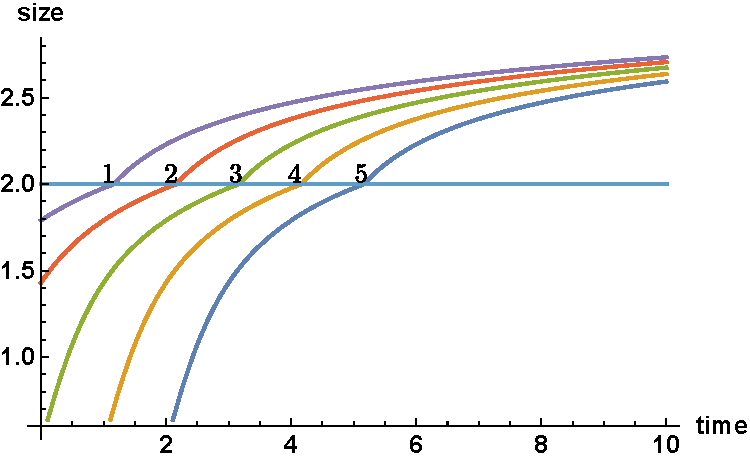
\includegraphics[scale = 0.75]{../illustrations/chara}
	\caption[Example of characteristics]{Characteristics for a constant competition $ \s_c = 2 $, a climatic constant $ \xi_{x, i} = 1 $, and for coefficients $ \beta_0 = \ln(3) $, $ \beta_1 = 1 $ and $ \beta_2 = -1 $. These curves are parameterised by $ \theta $ and allow us to follow a cohort with relative time $ \theta $}
	\label{fig::chara}
\end{figure}
We use the method of characteristics \citep{Olver2014b} which allows us to follow individuals through their life, \ie the characteristics represent the trajectories of individuals in the time-size plane (fig. \ref{fig::chara} for an example). The transport equation (equation 1 in the main text) requires an initial population at time $ t = 0 $, which we denote by $ \phi(s) $. It is the density of trees of size $ s $ at the beginning. Let the canopy height $ \s $ be known with a constant value $ \s_c $, and, let $ s $ and $ t $ be functions of a parameter $ \theta $. By applying the chain rule, we get:
\[
	\frac{d N\big(s(\theta), t(\theta) \big)}{d \theta} = \left. \frac{\partial N}{\partial s} \right|_{(s(\theta), t(\theta))} \frac{ds}{d \theta} +
			\left. \frac{\partial N}{\partial t} \right|_{(s(\theta), t(\theta))} \frac{dt}{d \theta}
\]
We therefore set the characteristic equations to:
\begin{align}
	\frac{ds}{d \theta} &= G(s, \s_c) \label{eq::chara_s} \\
		&= \xi_{x, i} e^{\beta_0 \mathbb{1}_{[\s_c, \infty[}(s) + \beta_1 s + \beta_2 s^2} \nonumber \\
	\frac{dt}{d \theta} &= 1 \label{eq::chara_t}
\end{align}
where $ \xi_{x, i} $ is a species-specific (due to the $ i $ index) constant depending of the climate at the location $ x $, and $ \mathbb{1}_A $ is the indicator function (\ie $ \mathbb{1}_A (s) $ equals 1 if $ s \in A $ and 0 otherwise). Hence, equation 1 (in the paper) is along the characteristics:
\begin{equation}
	\frac{dN}{d\theta} = - \left\{ \frac{\partial G}{\partial s}(s, \s, x) + \mu(s, \s, x) \right\} N(\theta) \label{eq::ODE_N}
\end{equation}
\begin{nota}[Abusing notations]
	We are abusing the notations $ N(\theta) $ and $ N\big( s(\theta), t(\theta) \big) $ to make equations easier to read. It would have been more correct to write
	\[
		\widetilde{N}(\theta) = N \big(s(\theta), t(\theta) \big)
	\]
\end{nota}

For the sake of readability, we drop the $ x $ in $ G $ and $ \mu $, and write $ \exp $ for the exponential function instead of $ e^x $. The solution of equation \eqref{eq::ODE_N} is:
\begin{equation} \label{eq::sol_ODE_N}
	N(\theta_1) = N(\theta = 0) \exp \left[-\int_0^{\theta_1} \mu(s, \s_c) + \frac{\partial G}{\partial s}(s, \s_c) \, d\theta \right]
\end{equation}
where the boundary condition $ N(\theta = 0) = N(s_{\theta = 0}, t_{\theta = 0}) $, and the coordinates $ (s(\theta_1), t(\theta_1)) $ are to be determined. We denoted $ s_{\theta = 0} $ to specify it is the origin of the characteristic but still distinguish it from $ s_0 $, the size of newborns. The time coordinate, solution of \eqref{eq::chara_t}, is denoted by $ T $:
\[
	T(\theta) = \theta + t_{\theta = 0}
\]
however, the $ i $-state coordinate $ s $ cannot be expressed in terms of elementary functions. In what follows, we assume $ \beta_2 < 0 $ which is true for all the species we parameterised. Thus, the integral
\begin{align*}
	\int  | G(s, \s_c) | \, ds &\leqslant \int e^{|\beta_0|} e^{\beta_1 s + \beta_2 s^2} \, ds \\
	&\leqslant e^{|\beta_0| - \frac{\beta_1^2}{4 \beta_2^2}} \int e^{\beta_2(s + \sfrac{\beta_1}{2\beta_2})^2} \, ds
\end{align*}
exists and equation \eqref{eq::chara_s} has a solution that we denote by $ S(\theta_1, s_{\theta = 0}, \s_c) $. This solution $ S(\theta_1, s_{\theta = 0}, \s_c) $ is the coordinate of the $ i $-state at $ \theta_1 $ along the characteristic originated in $ s_{\theta = 0} $ at $ t_{\theta = 0} $.

Let us assume that $ S $ admits an inverse, in other words, there exists a function $ \tau $ such that:
\begin{align*}
	\tau \big( S(\theta_1, s_{\theta = 0}, \s_c), s_{\theta = 0}, \s_c \big) &= \theta_1 \\
	S \big(\tau(s_1, s_{\theta = 0}, \s_c), s_{\theta = 0}, \s_c \big) &= s_1
\end{align*}
Then, by definition, $ \tau(s_1, s_0, \s_c) $ is the time it requires to grow from $ s_0 $ to $ s_1 $ under competition $ \s_c $. Although, equation 1 (in the paper) cannot be solved analytically (we would need an explicit solution of $ S $ and $ \tau $), the net reproduction rate is still tractable. Indeed, equation \eqref{eq::sol_ODE_N} can be rewritten:
\begin{align*}
	N \big( s(\theta_1), t(\theta_1) \big) &= N( s_{\theta = 0}, t_{\theta = 0}) \exp \left[-\int_0^{\theta_1} \mu(s, \s_c) + \frac{\partial G}{\partial s}(s, \s_c) \, d\theta \right] \\
	&= N( s_{\theta = 0}, t_{\theta = 0}) \exp \left[-\int_{s_{\theta = 0}}^{s(\theta_1)} \left( \mu(s, \s_c) + \frac{\partial G}{\partial s}(s, \s_c) \right) \frac{d \theta}{ds} \, ds \right] \\
	&= N( s_{\theta = 0}, t_{\theta = 0}) \exp \left[-\int_{s_{\theta = 0}}^{s(\theta_1)} \left( \mu(s, \s_c) + \frac{\partial G}{\partial s}(s, \s_c) \right) \frac{1}{G(s, \s_c)} \, ds \right] \\
	&= N( s_{\theta = 0}, t_{\theta = 0}) \frac{G(s_{\theta = 0}, \s_c)}{G \big( s(\theta_1), \s_c \big)} \exp \left[-\int_{s_{\theta = 0}}^{s(\theta_1)} \frac{\mu(s, \s_c)}{G(s, \s_c)} \, ds \right] \\
\end{align*}

If a characteristic emerged at $ t_{\theta = 0} \leqslant 0 $, then it concerns the initial population (at $ t = 0 $) denoted by $ \phi(s) $:
\begin{equation}\label{eq::sol_init}
	N(S(t, s, \s_c), t) = \phi(s) \frac{G(s, \s_c)}{G\big( S(t, s, \s_c), \s_c \big)} \exp \left[ -\int_{s}^{S(t, s, \s_c)} \frac{\mu(\sigma, \s_c)}{G(\sigma, \s_c)} \, d\sigma \right]
\end{equation}
where $ S(t, s, \s_c) $ is the size of the individual at time $ t $ given at time $ 0 $ they were of size $ s $. In figure \ref{fig::chara}, the characteristics that emerged before $ t = 0 $ are the first, second and third curves.

For characteristics that emerged after time 0 (fourth and fifth curves on fig \ref{fig::chara}), we denote their birth coordinates $ (s_{\theta = 0}, t_{\theta = 0}) $ by $ (0, t_b) $; $ t_b > 0 $ stands for the time of birth.
\begin{equation}\label{eq::sol_later}
	N(s, t) = N \big( 0, t - \tau(s, 0, \s_c) \big) \frac{G(0, \s_c)}{G(s, \s_c)} \exp \left[ -\int_{0}^{s} \frac{\mu(\sigma, \s_c)}{G(\sigma, \s_c)} \, d\sigma \right]
\end{equation}

The initial population (equation \eqref{eq::sol_init}) goes extinct as $ t $ goes by. Therefore, only equation \eqref{eq::sol_later} is of interest \citep{DeRoos1997}. We now use the boundary condition equation 2 (in the paper, once again, we drop the spatial variable $ x $ since the dispersal kernel $ \K $ is a Dirac):
\begin{align*}
	N(0, t) G(0, \s_c) &= \int_{0}^{\infty} F(s, \s_c) N(s, t) \, ds \\
		&= \int_{0}^{\infty} F(s, \s_c) N \big( 0, t - \tau(s, 0, \s_c) \big) \frac{G(0, \s_c)}{G(s, \s_c)} \exp \left[ -\int_{0}^{s} \frac{\mu(\sigma, \s_c)}{G(\sigma, \s_c)} \, d\sigma \right] \, ds
\end{align*}
Let
\[
	B(t, \s_c) = N(0, t) G(0, \s_c)
\]
the population birth rate (\ie the quantity of seedlings created at time $ t $ by a population undergoing a competition $ \s_c $). We can substitute $ B $ into the previous equation:
\begin{equation} \label{eq::popBirth}
	B(t, \s_c) = \int_{0}^{\infty} B \big(t - \tau(s, 0, \s_c), \s_c \big) \frac{F(s, \s_c)}{G(s, \s_c)} \exp \left[ -\int_{0}^{s} \frac{\mu(\sigma, \s_c)}{G(\sigma, \s_c)} \, d\sigma \right] \, ds
\end{equation}
If $ \tau $ were a known function (which is not the case here), equation \eqref{eq::popBirth} would relate the population birth rate to its past. The quantity
\[
	\frac{1}{G(s, \s_c)} B \big(t - \tau(s, 0, \s_c), \s_c \big) \exp \left[ -\int_{0}^{s} \frac{\mu(\sigma, \s_c)}{G(\sigma, \s_c)} \, d\sigma \right]
\]
is just the density of individuals born $ t - \tau $ times unit ago and that survived up to a size in $ [s, s + ds] $ at time $ t $, and $ B $ is the inflow per unit time.

Equation \eqref{eq::popBirth} admits an equilibrium only for particular combinations of parameters $ G $, $ \mu $ and $ F $ and since there is no density dependence here ($ \s $ is set to a known value $ \s_c $), then $ B $ ultimately grows or decline exponentially \citep{DeRoos1997}. We therefore substitute the trial solution
\begin{equation} \label{eq::B_trial}
	B(t, \s_c) = B_0e^{\lambda t}
\end{equation}
into \eqref{eq::popBirth} to get:
\begin{align*}
	B_0 e^{\lambda t} &= \int_{0}^{\infty} B_0 e^{\lambda t - \lambda \tau(s, 0, \s_c)} \frac{F(s, \s_c)}{G(s, \s_c)} \exp \left[ -\int_{0}^{s} \frac{\mu(\sigma, \s_c)}{G(\sigma, \s_c)} \, d\sigma \right] \, ds \\
	&= B_0 e^{\lambda t} \int_{0}^{\infty} e^{- \lambda \tau(s, 0, \s_c)} \frac{F(s, \s_c)}{G(s, \s_c)} \exp \left[ -\int_{0}^{s} \frac{\mu(\sigma, \s_c)}{G(\sigma, \s_c)} \, d\sigma \right] \, ds \\
\end{align*}
Thus, we get:
\begin{equation} \label{eq::eigen}
	1 = \int_{0}^{\infty} e^{- \lambda \tau(s, 0, \s_c)} \frac{F(s, \s_c)}{G(s, \s_c)} \exp \left[ -\int_{0}^{s} \frac{\mu(\sigma, \s_c)}{G(\sigma, \s_c)} \, d\sigma \right] \, ds
\end{equation}
When $ \lambda $ is set to 0, the right hand side of \eqref{eq::eigen} becomes:
\begin{equation} \label{eq::R0_app}
	\int_{0}^{\infty} \frac{F(s, \s_c)}{G(s, \s_c)} \exp \left[ -\int_{0}^{s} \frac{\mu(\sigma, \s_c)}{G(\sigma, \s_c)} \, d\sigma \right] \, ds
\end{equation}
It represents the expected number of seedlings produced by an individual through its lifespan, which is by definition the net reproduction rate $ R_0(\s_c) $ we were looking for (equation 4 in the paper). Given only canopy individuals can reproduce, $ \forall s < \s_c $, $ F(s, \s_c) = 0 $ and $ \forall s \geqslant \s_c $, $ F(s, \s_c) > 0 $, the lower limit of the integrals can be changed to $ \s_c $ in equation \eqref{eq::R0_app}:
\[
	R_0 = \exp \left[- \int_{0}^{\s_c} \frac{\mu(\sigma, \s_c)}{G(\sigma, \s_c)} \, d\sigma \right] \times \int_{\s_c}^{\infty} \frac{F(s, \s_c)}{G(s, \s_c)} \exp \left[ - \int_{\s_c}^{s} \frac{\mu(\sigma, \s_c)}{G(\sigma, \s_c)} \, d\sigma \right] \, ds
\]
\begin{rem}[On $ \lambda $]
	If $ \lambda = 0 $ is truly solution of \eqref{eq::eigen}, then $ R_0(\s_c) = 1 $ and the population is stable. This is consistent with \eqref{eq::B_trial} since in this case the population birth rate would be constant.
\end{rem}

The constant $ \lambda $ is called the intrinsic growth rate of the population. Let us now prove that $ \lambda > 0 $ is equivalent to a net reproduction rate $ R_0(\s_c) > 1 $. Denote by $ f $ the function:
\[
	f(\lambda) = \int_{0}^{\infty} e^{- \lambda \tau(s, 0, \s_c)} \frac{F(s, \s_c)}{G(s, \s_c)} \exp \left[ -\int_{0}^{s} \frac{\mu(\sigma, \s_c)}{G(\sigma, \s_c)} \, d\sigma \right] \, ds
\]
We have:
\begin{align*}
	f'(\lambda) &= -\lambda f(\lambda) \\
	f''(\lambda) &= +\lambda^2 f(\lambda)
\end{align*}
Given $ f $ is a positive function (fecundity and growth are positive functions), then $ f $ is a convex decreasing function on $ \R^{+} $ and its maximum is reached at $ \lambda = 0 $. Hence, if $ R_0 > 1 $:
\[
	f(\lambda) = 1
\]
admits a unique solution on $ \R^{+} $. Thus
\[
	R_0 > 1 \Leftrightarrow \lambda > 0
\]

\subsection{Proofs of the three assertions \label{app::calc_R0::sec::3asser}}
We now prove the three following assertions:
\begin{enumerate}[label=(\textit{\roman*})]
	\item $ R_0(\s_c) $ is a decreasing function
	\item $ R_0 $ is an increasing function of the average understorey growth $ \bar{G} $ and a decreasing function of the average mortality $ \bar{\mu} $
	\item $ R_0 $ is an increasing function of the average fecundity $ \bar{F} $
\end{enumerate}

\subsubsection{First assertion}
The easiest argument to prove $ R_0 $ is a decreasing function of $ \s $ is to see that all the integrand's parts are always positive. Let:
\[
	f(s_1) = \int_{s_1}^{\infty} \frac{F}{G} e^{-\int_{s_1}^s \frac{\mu}{G} \, d\sigma} \, ds
\]
For any $ s_1 \leqslant s_2 $ we have:
\begin{align*}
	R_0(s_1) - R_0(s_2) &= e^{-\int_{0}^{s_1} \frac{\mu}{G} \, ds} \left[ \left( 1 - e^{-\int_{s_1}^{s_2} \frac{\mu}{G} \, ds} \right) f(s_2) + \int_{s_1}^{s_2} \frac{\mu}{G} \, ds \right] \\
		&\geqslant 0
\end{align*}
Therefore, $ R_0 $ is a decreasing function of $ \s $.

\subsubsection{Second assertion}
The average understorey growth for a canopy height $ \s $ is defined by
\[
	\bar{G} = \frac{1}{\s} \int_0^{\s} G(s, \s) \, ds
\]
Let $ G_1 $ and $ G_2 $ two growth functions. Since the overstorey growth is not changed, we just study the ratio:
\begin{equation} \label{eq::ratio_G}
	\frac{e^{\int_0^{\s} \frac{\mu}{G_1} \, ds}}{\int_0^{\s}e^{\frac{\mu}{G_2} \, ds}}
\end{equation}
We want to find a sufficient condition on $ G_1 $ and $ G_2 $ to get this ratio larger than 1, which means the net reproduction rate $ R_0 $ increases. Equation \eqref{eq::ratio_G} can be be rewritten:
\[
	e^{\int_0^{\s} \frac{\mu (G_1 - G_2)}{G_1 G_2} \, ds} \geqslant 1 \quad \Leftrightarrow \quad \int_0^{\s} \frac{\mu (G_1 - G_2)}{G_1 G_2} \, ds \geqslant 0
\]
Given $ \mu $ and $ G $ are positive functions, we can lower bound the integrand:
\begin{equation} \label{eq::minor}
	\frac{\mu (G_1 - G_2)}{G_1 G_2} \geqslant \frac{\max(\mu)}{\min(G_1 G_2)} \mathds{1}_{G_1 < G_2} (s) \times (G_1 - G_2) + \frac{\min(\mu)}{\max(G_1 G_2)} \mathds{1}_{G_1 \geqslant G_2}(s) \times (G_1 - G_2)
\end{equation}
Define
\[
	\begin{matrix}
		k_1 = \frac{\max(\mu)}{\min(G_1 G_2)} & &
			\mathscr{D}_1 = \{ s | G_1(s) < G_2(s) \} \\
		k_2 = \frac{\min(\mu)}{\max(G_1 G_2)} & &
				\mathscr{D}_2 = \{ s | G_1(s) \geqslant G_2(s) \}\\
	\end{matrix}
\]
equation \eqref{eq::minor} is:
\begin{align*}
	\int_0^{\s} \frac{\mu (G_1 - G_2)}{G_1 G_2} &\geqslant
		k_1 \int_{\mathscr{D}_1} G_1  \, ds + k_2 \int_{\mathscr{D}_2} G_1 \, ds +
		k_1 \int_{\mathscr{D}_1} G_2  \, ds + k_2 \int_{\mathscr{D}_2} G_2 \, ds \\
	&\geqslant \min (k_1, k_2) \left[\int_{\mathscr{D}_1 \cup \mathscr{D}_2} G_1 \, ds + \int_{\mathscr{D}_1 \cup \mathscr{D}_2} G_2 \, ds \right]
\end{align*}
Therefore, given $ \mathscr{D}_1 \cup \mathscr{D}_2 = [0, \s] $, a sufficient condition to have the ratio defined by equation \eqref{eq::ratio_G} larger than $ 1 $ is:
\begin{equation}
	\int_0^{\s} G_1 \, ds \geqslant \int_0^{\s} G_2 \, ds,
\end{equation}
that is to say:
\[
	\bar{G}_1 \geqslant \bar{G}_2
\]
Thus, when the understorey growth increases in average, so does the net reproduction rate $ R_0 $. A similar reasoning on $ \mu $ would prove that increasing the understorey mortality induce a depleted $ R_0 $. This conclude the proof of the second assertion.

\subsubsection{Third assertion}
In this article, we used the fecundity of \citet{Purves2008} which is proportional to sun-exposed crown area $ \A $:
\[
	F(s, \s) = f \A(s, \s)
\]
where $ f $ is the new recruits per unit time per crown area.
\begin{align*}
	\frac{\partial R_0}{\partial f} &= e^{-\int_0^{\s} \frac{\mu}{G} \, ds} \int_{\s}^{\infty} \frac{A}{G} e^{-\int_{\s}^{s} \frac{\mu}{G} \, d \sigma} \, ds \\
		&\geqslant 0
\end{align*}
Thus, increasing fecundity augments $ R_0 $, which proves the third assertion.

\subsection{Proofs of the relations between \citet{Purves2009} and our study}
In this section, we first provide the assumptions concerning the demography in \citet{Purves2009}, and match our notations with his article in the table \ref{tab::notations_purves2009}. Finally, we derive Purves's formul\ae{} from our $ R_0 $ equation 4 (in the paper). Except when specified, Purves refers to \citet{Purves2009} in the following sections.
\begin{table}[!h]
	\centering
	\caption[Link between our notations and Purves's notations]{Link between our notations and \citet{Purves2009}'s notations. Note that he uses the flat-top version of the perfect-plasticity approximation, which implies the fecundity function to be proportional to the trunk area.}
	\label{tab::notations_purves2009}
	\begin{tabular}{@{}rll@{}}
	\toprule
	\textbf{Meaning} & \textbf{Our notation} & \textbf{\citet{Purves2009}} \\
	Species index & $ j $, but mostly dropped & $ j $ \\
	Space & $ x $ & $ R $ (not to be confound with $ R_0 $) \\
	Time & $ t $ & $ \tau $ \\
	Threshold diameter & $ \s, \, \s_c $ & $ D^{*} $ \\
	Net reprod. rate & $ R_0 (x, \s_c) $ & $ R_{0, j, R} $ \\
	Indiv. growth rate overstorey & $ G(s, \s, x), \, s \geqslant \s $ & $ G_{L, j, R} $ \\
	Indiv. growth rate understorey & $ G(s, \s, x), \, s < \s $ & $ G_{D, j, R} $ \\
	Mortality rate overstorey & $ \mu(s, \s, x), \, s \geqslant \s $ & $ \mu_{L, j, R} = \sfrac{1}{\rho_{L, j, R}} $ \\
	Mortality rate understorey & $ \mu(s, \s, x), \, s < \s $ & $ \mu_{D, j, R} = \sfrac{1}{\rho_{D, j, R}} $ \\
	Fecundity function & $ \F \A(s, \s) $ & $ F_{j, R}^{\text{capita}} \pi \sfrac{s^2}{4} $ \\
   \bottomrule
	\end{tabular}
\end{table}

\subsubsection{Additional assumptions to our model from \citet{Purves2009}}
We sum-up here some useful assumptions from Purves. The assumptions are better described in \citet[not to confound with 2009's paper]{Purves2008}.
\begin{assum}[Flat-top crown] \label{assum::flat-top}
	The crown is a flat-top disc expressed at the top of the tree, which implies that the area of the crown $ \A(s, \s) $ is independent of its second argument.
\end{assum}

\begin{assum}[Demographic rates]
	The individual growth and mortality rates are step functions with the discontinuity at $ \s $:
	\[
		G_{j, R}(s, \s) =
		\begin{cases}
			G_{L, j, R} & \text{if } s \geqslant \s \\
			G_{D, j, R} & \text{otherwise}
		\end{cases}
	\]
	\[
	\mu_{j, R}(s, \s) =
		\begin{cases}
			\mu_{L, j, R} & \text{if } s \geqslant \s \\
			\mu_{D, j, R} & \text{otherwise}
		\end{cases}
	\]
	where $ G_{L, j, R}, \, G_{D, j, R}, \, \mu_{L, j, R}, \, \mu_{D, j, R} $ are estimated constants.
\end{assum}

\begin{assum}[Mortality versus individual growth] \label{assum::negligible}
	The mortality rate is negligible compare to both 1 and the individual growth rate:
	\begin{align}
		\mu_{L, j, R} &\ll 1 \\
		\mu_{L, j, R} &\ll G_{L, j, R}
	\end{align}
\end{assum}

\begin{assum}[Fecundity function]
	Due to the flat-top assumption \ref{assum::flat-top}, the fecundity is simply proportional to the cross-section of the trunk area at breast height:
	\[
		F_{j, R} (s, \s) =
		\begin{cases}
			\frac{1}{10^4} F_{j, R}^{\text{capita}} \pi s^2 & \text{if } s \geqslant \s \\
			0 & \text{otherwise}
		\end{cases}
	\]
	The factor $ \frac{1}{10^4} $ corrects for the units of $ F_{j, R}^{\text{capita}} $ (basal area per year, dividing by $ 10^4 $ makes the basal area dimensionless).
\end{assum}

Note that in his supporting information, Purves integrates with respect to time rather than size. In the case trees are always in the overstorey, it is strictly equivalent:
\[
	\begin{cases}
		\frac{ds}{d \tau} = G_{L, j, R} \\
		s(0) = D^{*}
	\end{cases}
\]
which has the solution:
\[
	s(\tau) = \tau G_{L, j, R} + D^{*}
\]
This solution is for instance found in equation S11 \citep{Purves2009}.

\subsubsection{$ R_0 $ equation \citep[p. 1479]{Purves2009}}
Equation 4 (in the paper) is equivalent to equation S10.2 \citep[also p. 1479 in his article]{Purves2009} when $ \s_c = 0 $.
\begin{proof}
	Let $ \s_c = 0 $.
	\begin{align*}
		R_0 (x, 0) &= \overbrace{e^{-\int_0^{0}\frac{\mu(s, \s_c, x)}{G(s, \s_c, x)} \, ds}}^{= 1} \int_{0}^{\infty} \frac{1}{10^4} \frac{F_{j, R}^{\text{capita}} \pi (\sfrac{s}{2})^2}{G_{L, j, R}} e^{-\int_{0}^{s} \frac{\mu_{L, j, R}}{G_{L, j, R}} \, d\sigma} \, ds \\
			&= \frac{1}{10^4} \frac{\pi}{4} \frac{F_{j, R}^{\text{capita}}}{G_{L, j, R}} \int_{0}^{\infty} s^2 e^{-\frac{\mu_{L, j, R}}{G_{L, j, R}} s} \, ds \\
			&= \frac{1}{10^4} \frac{\pi}{2} F_{j, R}^{\text{capita}} \frac{G_{L, j, R}^2}{\mu_{L, j, R}^3} \\
			&= \frac{1}{10^4} \frac{\pi}{2} F_{j, R}^{\text{capita}} G_{L, j, R}^2 \rho_{L, j, R}^3
	\end{align*}
\end{proof}

\subsubsection{Proportion of the trees that make up to the canopy}
Let $ P^{\text{canop}} $ be the proportion of individuals that survive up to the canopy. The quantity $ P^{\text{canop}} $ is derived in Purves' supporting information, a little before equation S11; we can obtain the same result with the first part of equation 4 (in the paper).
\begin{proof}
	\begin{align*}
		P^{\text{canop}} &= e^{-\int_{0}^{D^{*}} \frac{\mu}{G} \, ds} \\
			&= e^{-\frac{\mu_{D, j, R}}{G_{D, j, R}} D^{*}} \\
			&= e^{-\frac{D^{*}}{G_{D, j, R}\rho_{D, j, R}}}
	\end{align*}
\end{proof}

\subsubsection{$ D^{*} $ at equilibrium \citep[equation S13.2]{Purves2009}}
Let $ \hat D^{*} $ be the threshold diameter when the (monospecific) population is at equilibrium. We derive equation S13.2 \citep{Purves2009} from our equation 4 (in the paper) using Purves' notations:
\begin{align*}
	R^{\text{canop}} &= e^{-\int_{0}^{D^{*}} \frac{\mu_{D, j, R}}{G_{D, j, R}} \, ds} \int_{D^{*}}^{\infty} \frac{1}{10^4} \frac{F_{j, R}^{\text{capita}} \pi (\sfrac{s}{2})^2}{G_{L, j, R}} e^{-\int_{D^{*}}^{s} \frac{\mu_{L, j, R}}{G_{L, j, R}} \, d\sigma} \, ds \\
		&= e^{\left(\frac{\mu_{L, j, R}}{G_{L, j, R}} - \frac{\mu_{D, j, R}}{G_{D, j, R}} \right) D^{*}} \frac{1}{10^4} \frac{\pi}{4 G_{L, j, R}} F_{j, R}^{\text{capita}} \int_{D^{*}}^{\infty} s^2 e^{-\frac{\mu_{L, j, R}}{G_{L, j, R}} s} \\
		&= \frac{1}{10^4} \frac{\pi}{4} F_{j, R}^{\text{capita}} e^{- \frac{\mu_{D, j, R}}{G_{D, j, R}} D^{*}} \frac{1}{\mu_{L, j, R}^3} (2 G_{L, j, R}^2 + 2 G_{L, j, R} \mu_{L, j, R} D^{*} + \mu_{L, j, R}^2 {D^{*}}^2)
\end{align*}
Using assumption \ref{assum::negligible}, we get a simplified version of $ R^{\text{canop}} $:
\begin{equation} \label{eq::RcanopApprox}
	R^{\text{canop}} \approx \frac{1}{10^4} \frac{\pi}{2} F_{j, R}^{\text{capita}} e^{- \frac{\mu_{D, j, R}}{G_{D, j, R}} D^{*}} \frac{1}{\mu_{D, j, R}^3} G_{L, j, R}^2
\end{equation}
At equilibrium, each individual replace itself once in average. Therefore, $ R^{\text{canop}} = 1 $. Solving equation \eqref{eq::RcanopApprox} at equilibrium for $ \hat D^{*} $, we get:
\[
	\hat D^{*} = G_{D, j, R} \rho_{D, j, R} \ln \left( \frac{1}{10^4} \frac{\pi}{2} F_{j, R}^{\text{capita}} G_{L, j, R}^2 \rho_{L, j, R}^3 \right) \text{, where } \frac{1}{\mu_{L, j, R}^3} = \rho_{L, j, R}^3,
\]
which is the equation S13.2 of Purves.
\end{onehalfspace}

\printbibliography[heading=subbibliography]
\end{refsection}

\end{document}


% \section{Proofs of the relations between \citet{Purves2009} and our study} \label{app::purves2009}
\begin{refsection}
In this section, we first provide the assumptions concerning the demography in \citet{Purves2009}, and match our notations with \citeauthor{Purves2009}'s article in the table \ref{tab::notations_purves2009}. Finally, we derive \citet{Purves2009}'s formul\ae{} from our $ R_0 $ equation \eqref{eq::R0sol}.
\begin{table}
	\centering
	\caption{Link between our notations and \citet{Purves2009}'s notations. Note that \citeauthor{Purves2009} uses the flat-top version of the perfect-plasticity approximation, which implies the fecundity function to be proportional to the trunk area.}
	\label{tab::notations_purves2009}
	\begin{tabular}{@{}rll@{}}
	\toprule
	\textbf{Meaning} & \textbf{Our notation} & \textbf{\citet{Purves2009}} \\
	Species index & $ j $, but mostly dropped & $ j $ \\
	Space & $ x $ & $ R $ (not to be confound with $ R_0 $) \\
	Time & $ t $ & $ \tau $ \\
	Threshold diameter & $ \s, \, \s_c $ & $ D^{*} $ \\
	Net reprod. rate & $ R_0 (x, \s_c) $ & $ R_{0, j, R} $ \\
	Indiv. growth rate overstorey & $ G(s, \s, x), \, s \geqslant \s $ & $ G_{L, j, R} $ \\
	Indiv. growth rate understorey & $ G(s, \s, x), \, s < \s $ & $ G_{D, j, R} $ \\
	Mortality rate overstorey & $ \mu(s, \s, x), \, s \geqslant \s $ & $ \mu_{L, j, R} = \sfrac{1}{\rho_{L, j, R}} $ \\
	Mortality rate understorey & $ \mu(s, \s, x), \, s < \s $ & $ \mu_{D, j, R} = \sfrac{1}{\rho_{D, j, R}} $ \\
	Fecundity function & $ \F \A(s, \s) $ & $ F_{j, R}^{\text{capita}} \pi \sfrac{s^2}{4} $ \\
   \bottomrule
	\end{tabular}
\end{table}

\subsection{Additional assumptions to our model from \citet{Purves2009}}
We sum-up here some useful assumptions from \citet{Purves2009}. The assumptions are better described in \citet[and yes, it is in the paper of 2008]{Purves2008}
\begin{assum}[Flat-top crown] \label{assum::flat-top}
	The crown is a flat-top disc expressed at the top of the tree, which implies that the area of the crown $ \A(s, \s) $ is independent of its second argument.
\end{assum}

\begin{assum}[Demographic rates]
	The individual growth and mortality rates are step functions with the discontinuity at $ \s $:
	\[
		G_{j, R}(s, \s) =
		\begin{cases}
			G_{L, j, R} & \text{if } s \geqslant \s \\
			G_{D, j, R} & \text{otherwise}
		\end{cases}
	\]
	\[
	\mu_{j, R}(s, \s) =
		\begin{cases}
			\mu_{L, j, R} & \text{if } s \geqslant \s \\
			\mu_{D, j, R} & \text{otherwise}
		\end{cases}
	\]
	where $ G_{L, j, R}, \, G_{D, j, R}, \, \mu_{L, j, R}, \, \mu_{D, j, R} $ are estimated constants.
\end{assum}

\begin{assum}[Fecundity function]
	Due to the flat-top assumption \ref{assum::flat-top}, the fecundity is simply proportional to the cross-section of the trunk area at breast height:
	\[
		F_{j, R} (s, \s) =
		\begin{cases}
			\frac{1}{10^4} F_{j, R}^{\text{capita}} \pi s^2 & \text{if } s \geqslant \s \\
			0 & \text{otherwise}
		\end{cases}
	\]
	The factor $ \frac{1}{10^4} $ corrects for the units of $ F_{j, R}^{\text{capita}} $ (basal area per year, dividing by $ 10^4 $ makes the basal area dimensionless).
\end{assum}

\begin{assum}[Mortality versus individual growth] \label{assum::negligible}
	The mortality rate is negligible compare to both 1 and the individual growth rate:
	\begin{align}
		\mu_{L, j, R} &\ll 1 \\
		\mu_{L, j, R} &\ll G_{L, j, R}
	\end{align}
\end{assum}

Note that in his supporting information, \citet{Purves2009} integrates with respect to time rather than size. In the case trees are always in the overstorey, it is strictly equivalent:
\[
	\begin{cases}
		\frac{ds}{d \tau} = G_{L, j, R} \\
		s(0) = D^{*}
	\end{cases}
\]
which has the solution:
\[
	s(\tau) = \tau G_{L, j, R} + D^{*}
\]
This solution is for instance found in equation S11 \citep{Purves2009}.

\subsection{$ R_0 $ equation \citep[p. 1479]{Purves2009}}
Equation \eqref{eq::R0sol} is equivalent to equation S10.2 \citep[also p. 1479 in his article]{Purves2009} when $ \s_c = 0 $.
\begin{proof}
	Let $ \s_c = 0 $.
	\begin{align*}
		R_0 (x, 0) &= \overbrace{e^{-\int_0^{0}\frac{\mu(s, \s_c, x)}{G(s, \s_c, x)} \, ds}}^{= 1} \int_{0}^{\infty} \frac{1}{10^4} \frac{F_{j, R}^{\text{capita}} \pi (\sfrac{s}{2})^2}{G_{L, j, R}} e^{-\int_{0}^{s} \frac{\mu_{L, j, R}}{G_{L, j, R}} \, d\sigma} \, ds \\
			&= \frac{1}{10^4} \frac{\pi}{4} \frac{F_{j, R}^{\text{capita}}}{G_{L, j, R}} \int_{0}^{\infty} s^2 e^{-\frac{\mu_{L, j, R}}{G_{L, j, R}} s} \, ds \\
			&= \frac{1}{10^4} \frac{\pi}{2} F_{j, R}^{\text{capita}} \frac{G_{L, j, R}^2}{\mu_{L, j, R}^3} \\
			&= \frac{1}{10^4} \frac{\pi}{2} F_{j, R}^{\text{capita}} G_{L, j, R}^2 \rho_{L, j, R}^3
	\end{align*}
\end{proof}

\subsection{Proportion of the trees that make up to the canopy}
Let $ P^{\text{canop}} $ be the proportion of individuals that survive up to the canopy. The quantity $ P^{\text{canop}} $ is derived in \citet{Purves2009}'s supporting information, a little before equation S11; we can obtain the same result with the first part of equation \eqref{eq::R0sol}.
\begin{proof}
	\begin{align*}
		P^{\text{canop}} &= e^{-\int_{0}^{D^{*}} \frac{\mu}{G} \, ds} \\
			&= e^{-\frac{\mu_{D, j, R}}{G_{D, j, R}} D^{*}} \\
			&= e^{-\frac{D^{*}}{G_{D, j, R}\rho_{D, j, R}}}
	\end{align*}
\end{proof}

\subsection{$ D^{*} $ at equilibrium \citep[equation S13.2]{Purves2009}}
Let $ \hat D^{*} $ be the threshold diameter when the (monospecific) population is at equilibrium. We derive equation S13.2 \citep{Purves2009} from our equation \eqref{eq::R0sol} using \citeauthor{Purves2009}'s notations:
\begin{align*}
	R^{\text{canop}} &= e^{-\int_{0}^{D^{*}} \frac{\mu_{D, j, R}}{G_{D, j, R}} \, ds} \int_{D^{*}}^{\infty} \frac{1}{10^4} \frac{F_{j, R}^{\text{capita}} \pi (\sfrac{s}{2})^2}{G_{L, j, R}} e^{-\int_{D^{*}}^{s} \frac{\mu_{L, j, R}}{G_{L, j, R}} \, d\sigma} \, ds \\
		&= e^{\left(\frac{\mu_{L, j, R}}{G_{L, j, R}} - \frac{\mu_{D, j, R}}{G_{D, j, R}} \right) D^{*}} \frac{1}{10^4} \frac{\pi}{4 G_{L, j, R}} F_{j, R}^{\text{capita}} \int_{D^{*}}^{\infty} s^2 e^{-\frac{\mu_{L, j, R}}{G_{L, j, R}} s} \\
		&= \frac{1}{10^4} \frac{\pi}{4} F_{j, R}^{\text{capita}} e^{- \frac{\mu_{D, j, R}}{G_{D, j, R}} D^{*}} \frac{1}{\mu_{L, j, R}^3} (2 G_{L, j, R}^2 + 2 G_{L, j, R} \mu_{L, j, R} D^{*} + \mu_{L, j, R}^2 {D^{*}}^2)
\end{align*}
Using assumption \ref{assum::negligible}, we get a simplified version of $ R^{\text{canop}} $:
\begin{equation} \label{eq::RcanopApprox}
	R^{\text{canop}} \approx \frac{1}{10^4} \frac{\pi}{2} F_{j, R}^{\text{capita}} e^{- \frac{\mu_{D, j, R}}{G_{D, j, R}} D^{*}} \frac{1}{\mu_{D, j, R}^3} G_{L, j, R}^2
\end{equation}
At equilibrium, each individual replace itself once in average. Therefore, $ R^{\text{canop}} = 1 $. Solving equation \eqref{eq::RcanopApprox} at equilibrium for $ \hat D^{*} $, we get:
\[
	\hat D^{*} = G_{D, j, R} \rho_{D, j, R} \ln \left( \frac{1}{10^4} \frac{\pi}{2} F_{j, R}^{\text{capita}} G_{L, j, R}^2 \rho_{L, j, R}^3 \right) \text{, where } \frac{1}{\mu_{L, j, R}^3} = \rho_{L, j, R}^3,
\]
which is equation S13.2 \citep{Purves2009}.

% \subsection{Does assumptions \ref{assum::negligible} holds in our case?}
% In this subsection, we set the species $ j $ to \textit{Acer rubrum} (as in \citet[page 15 supporting information]{Purves2009}), and set arbitrarily the associated demographic rates:
% \begin{align*}
% 	G_{D, j, R} &= \int_{0}^{} G(s, \s_c, x) \, ds \\
% 	G_{L, j, R} &= \int_{}^{\infty} G(s, \s_c, x) \, ds \\
% 	\mu_{D, j, R} &= \int_{0}^{} \mu(s, \s_c, x) \, ds \\
% 	\mu_{L, j, R} &= \int_{}^{\infty} \mu(s, \s_c, x) \, ds
% \end{align*}
% where $ x = (77.93 \, W, 39.07 \, N) $, the closest point to the centroid of \textit{Acer rubrum}'s data where I have data. The value $ xxx $ is the diameter of a $ 12.5 \, m $ height \textit{Acer rubrum}.
\printbibliography[heading=subbibliography]
\end{refsection}

% 
\documentclass[letterpaper, 12pt]{article}

%%%%%%%%%%%%%%%%%%%    PACKAGES    %%%%%%%%%%%%%%%%%%%
%% Package version
\listfiles % Then check the .log file

%% Font
\usepackage{fontspec}
\usepackage{marvosym}

%% Languages
\usepackage{polyglossia}
	\setdefaultlanguage[variant=british]{english}

%% Marges, space...
\usepackage[top=2.5cm, bottom=2.5cm, left=2.5cm, right=2.5cm]{geometry}
\usepackage{setspace} % [nodisplayskipstretch] pour option space in equation

\usepackage{indentfirst}

\usepackage[bottom]{footmisc}
\usepackage{footnote}

% https://tex.stackexchange.com/questions/279/how-do-i-ensure-that-figures-appear-in-the-section-theyre-associated-with
\usepackage[section]{placeins} % To place figures in the section it is declared

%% Graphics
\usepackage[luatex]{graphicx}
	\graphicspath{{../graphs/}}

\usepackage{caption}
\usepackage{subcaption}
	\captionsetup{subrefformat=parens}

\makeatletter 
\renewcommand{\thefigure}{S\thesection.\@arabic\c@figure}
\renewcommand{\thetable}{S\thesection.\@arabic\c@table}
\renewcommand{\theequation}{S.\arabic{equation}}
\makeatother

\usepackage[dvipsnames, svgnames]{xcolor}

\usepackage{tikz}
	\usetikzlibrary{arrows, plotmarks, decorations.markings}
	\tikzstyle{arrow} = [->,>=stealth,thick,rounded corners=4pt,line width=1pt]
	\usetikzlibrary{shadows}
	\usetikzlibrary{shadings}
	\usetikzlibrary{positioning} % relative coodinate
	\usetikzlibrary{tikzmark, calc} % calc, to calculate coordinate
	\usetikzlibrary{decorations.pathmorphing} % to snake an arrow
	\usetikzlibrary{shapes.arrows}
	\usetikzlibrary{patterns}
	\tikzset{
		invisible/.style={opacity=0},
		visible on/.style={alt={#1{}{invisible}}},
		alt/.code args={<#1>#2#3}{%
		\alt<#1>{\pgfkeysalso{#2}}{\pgfkeysalso{#3}} % \pgfkeysalso doesn't change the path
		},
	} % end tikzset. Code from http://tex.stackexchange.com/questions/136143/tikz-animated-figure-in-beamer

%% Table of content
\addto\captionsenglish{ % Replace "english" with the language used in babel
	\renewcommand{\contentsname}{Supporting Information Appendix S2 contents}
}

%% Format section
\usepackage{titlesec}
\titlelabel{S\thetitle~}
\usepackage{titletoc}
\titlecontents{section}[0pt]{}{\bfseries S\thecontentslabel~}{\bfseries}{\hspace{1em plus 1fill}\contentspage}


\usepackage{enumitem}% http://ctan.org/pkg/enumitem

%% Links
\usepackage{url}
\usepackage[luatex, colorlinks=true, linkcolor=NavyBlue, urlcolor=MidnightBlue, citecolor=PineGreen]{hyperref}

%% Table
\usepackage{booktabs}

%% bibliography
\usepackage{csquotes}
\usepackage[style=apa, natbib=true, sorting=ynt]{biblatex}
\addbibresource{bib_database.bib}

%% mathematics
\usepackage{amsthm}
\usepackage{amsmath}
	\allowdisplaybreaks % Autoriser découpe formules entres pages
\usepackage{amssymb}
\usepackage{bbold}
\usepackage{dsfont}
\usepackage{mathrsfs}
\usepackage{bm}
\usepackage{xfrac}
\usepackage{etoolbox} % For renumbering (cf below, counter for model)

\usepackage{thmbox} % cf after for "theorem" definitions

\usepackage{gensymb}

\usepackage{siunitx}

%%%%%%%%%%%%%%%%%   NEW COMMANDES    %%%%%%%%%%%%%%%%%
%% Text
\newcommand {\ie}{\textit{i.e., }}
\newcommand {\eg}{\textit{e.g., }}
\newcommand {\cf}{\textit{cf} }
\newcommand\bsc[1]{\textsc{\MakeLowercase{#1}}} % Only if there is no french babel
\newcommand {\thup}[1]{{#1}\textsuperscript{th}}

%% Math
\newcommand {\s}{{s}^{*}}
\newcommand {\sst}{\tilde{s}^{*}} % s* stable d'où le st
\newcommand {\N}{\tilde{N}}
\newcommand {\A}{\mathscr{A}}
\newcommand {\K}{\mathcal{K}}
\renewcommand{\S}{\mathscr{S}}
\newcommand{\R}{\mathds{R}}
\newcommand{\Prob}{\mathds{P}}
\newcommand{\F}{\mathcal{F}}

\DeclareMathOperator{\logit}{logit}

%%%%%%%%%%%%%%%%%   THEOREM STYLE    %%%%%%%%%%%%%%%%%
\newtheoremstyle{theo}{\topsep}{\topsep}{\itshape}{}{\bfseries}{.}{\newline}{\thmname{#1} \thmnumber{#2} \thmnote{~: \textit{#3}}}
\theoremstyle{theo}
\newtheorem{rem}{Remark}[section]
\newtheorem{defi}{Definition}[section]
\newtheorem{assum}{Assumption}[section]
\newtheorem{nota}{Notation}[section]

%%%%%%%%%%%%%%%%%   SET COUNTER		%%%%%%%%%%%%%%%%%
\setcounter{section}{1}

\begin{document}
\tableofcontents
\listoftables
\listoffigures

\begin{refsection}
\begin{onehalfspace}

\section{Database} \label{app::database}
\subsection{Description of the data}
We used an abbreviation for each species, that we list in Tab. \ref{tab::species}. For each species, we list their spatial range in Tab. \ref{tab::spaceRange}, and we plot the ranges of temperature and precipitation that are used in the individual growth and mortality functions (Fig. \ref{fig::speciesClimRange}).  We also join the 19 bioclimatic variables used in the random forest and the demography models selection (Tab. \ref{tab::bioclim}). Finally, we mapped all the data we used, from 1963 to 2010 (Fig \ref{fig::mapDatabase}).

\begin{table}[h!]
\centering
\caption[Scientific and vernacular name of the 14 species]{Species list, and the abbreviation used in the other tables\label{tab::species}. The last three columns are the maximal dbh, the maximal age, and the page of \citet{Burns1990, Burns1990a} at which we found the informations.}
\label{tab::database}
\begin{tabular}{rlllll}
	\toprule
	\textbf{Species} & \textbf{Scientific name} & \textbf{Vernacular name} & $ \text{\textbf{dbh}}_{\bm{\max}} $ & $ \text{\textbf{age}}_{\bm{\max}} $ & \textbf{page} \\
	\midrule
	ABI-BAL & Abies balsamea & Balsam fir & 460 & 200 & 33 \\
	ACE-RUB & Acer rubrum & Red maple & 760 & 125 & 170 \\
	ACE-SAC & Acer saccharum & Sugar maple & 910 & 350 & 202 \\
	BET-ALL & Betula alleghaniensis & Yellow birch & 760 & 300 & 302 \\
	BET-PAP & Betula papyrifera & White birch & 300 & 150 & 348 \\
	FAG-GRA & Fagus grandifolia & American beech & 510 & 366 & 660 \\
	PIC-GLA & Picea glauca & White spruce & 900 & 275 & 410 \\
	PIC-MAR & picea mariana & Black spruce & 230 & 250 & 451 \\
	PIC-RUB & picea rubens & Red spruce & 610 & 400 & 499 \\
	PIN-BAN & Pinus banksiana & Jack pine & 250 &  80 & 566 \\
	PIN-STR & Pinus strobus & Eastern white pine & 1020 & 200 & 982 \\
	POP-TRE & Populus tremuloides & Quaking aspen & 300 & 200 & 1093 \\
	THU-OCC & Thuja occidentalis & Northern white cedar & 600 & 400 & 1197 \\
	TSU-CAN & Tsuga canadensis & Eastern hemlock & 1020 & 400 & 1246 \\
	\bottomrule
\end{tabular}
\end{table}

\begin{table}[ht]
\centering
\caption[Species-specific satial extent and number of measurements]{Number of individual measurements in the database, and geographical extent for each species (before cropping, see Fig. \ref{fig::mapDatabase} for the crop extent). There are \num{3816854} individual measurements in total. We used the projection system WGS 84 (EPSG:4326) for this table.}
\label{tab::spaceRange}
\begin{tabular}{lrrrrr}
	\toprule
	~ & ~ & \multicolumn{2}{c}{\textbf{Longitude}} & \multicolumn{2}{c}{\textbf{latitude}} \\
	\cmidrule(lr){3-4} \cmidrule(lr){5-6}
	\bfseries{Species} & \bfseries{$ \# $ measures} & \bfseries{min} & \bfseries{max} & \bfseries{min} & \bfseries{max} \\
	\midrule
		ABI-BAL & \num{822265} & -96.07 & -57.31 & 39.04 & 52.90 \\
		ACE-RUB & \num{469195} & -96.47 & -63.86 & 25.91 & 49.49 \\
		ACE-SAC & \num{321776} & -97.65 & -63.96 & 30.66 & 49.44 \\
		BET-ALL & \num{104249} & -95.52 & -63.87 & 31.48 & 49.38 \\
		BET-PAP & \num{291701} & -154.01 & -57.99 & 37.92 & 61.42 \\
		FAG-GRA & \num{96990} & -95.04 & -64.59 & 30.36 & 51.29 \\
		PIC-GLA & \num{104342} & -151.78 & -58.19 & 37.70 & 61.44 \\
		PIC-MAR & \num{656273} & -151.40 & -57.31 & 41.70 & 61.13 \\
		PIC-RUB & \num{126063} & -84.35 & -62.61 & 35.31 & 51.43 \\
		PIN-BAN & \num{204463} & -99.09 & -64.49 & 38.95 & 52.57 \\
		PIN-STR & \num{90002} & -96.94 & -61.95 & 31.49 & 51.50 \\
		POP-TRE & \num{310514} & -151.15 & -59.58 & 32.43 & 61.42 \\
		THU-OCC & \num{153013} & -95.79 & -64.22 & 35.20 & 50.82 \\
		TSU-CAN & \num{66008} & -91.93 & -64.70 & 31.60 & 49.57 \\
	\bottomrule
\end{tabular}
\end{table}

\begin{figure}[htb]
    \centering
	%% First row
	\begin{subfigure}{0.98\textwidth}
		\input{../graphs/annual_mean_temperature-min_temperature_of_coldest_month_sp_range}
		\caption{Annual mean temperature $ T_a $ (left), and minimal temperature $ T_m $(right) range for each species. The vertical line is the average among species, and the dark circles are the species-specific mean.}
		\label{fig::annual_mean_temperature}
	\end{subfigure}
	\medskip
	%% Second row
	\begin{subfigure}{0.98\textwidth}
		\input{../graphs/annual_precipitation-precipitation_of_driest_quarter_sp_range}
		\caption{Annual precipitation $ P_a $ (left), and minimal precipitation $ P_m $(right) range for each species. The vertical line is the average among species, and the dark circles are the species-specific mean.}
		\label{fig::annual_precipitation}
	\end{subfigure}
\caption[Species climatic range]{Species-specific \subref{fig::annual_mean_temperature} temperature ranges and \subref{fig::annual_precipitation} precipitation ranges. The definitions of $ T_a, \, T_m, \, P_a, \, P_m $ are in table \ref{tab::bioclim}.}
\label{fig::speciesClimRange}
\end{figure}

\begin{table}[h!]
\centering
\caption[Bioclimatic variables list]{Bioclimatic variables list \citep{McKenney2011}. \label{tab::bioclim}}
\begin{tabular}{p{6.75cm}p{9cm}}
	\toprule
	\textbf{Name} & \textbf{Description} \\
	\midrule
	annual mean temperature $ T_a $ & avg of mean monthly temperatures \\
	mean diurnal range $ r_T $ & avg of monthly temperature ranges \\
	isothermality $ I $ & variable 2 divided by variable 7 \\
	temperature seasonality $ T_s $ & standard deviation of monthly-mean temperature estimates expressed as a percent of their mean \\
	max temperature of warmest month $ T_M $ & highest monthly maximum temperature \\
	min temperature of coldest month $ T_m $ & lowest monthly minimum temperature \\
	temperature annual range $ T_r $ & Variable 5 minus variable 6 \\
	mean temperature of wettest quarter $ T_w $ & avg temperature during 3 wettest months \\
	mean temperature of driest quarter $ T_d $ & avg temperature during 3 driest months \\
	mean temperature of warmest quarter $ T_h $ & avg temperature during 3 warmest months \\
	mean temperature of coldest quarter $ T_c $ & avg temperature during 3 coldest months \\
	annual precipitation $ P_a $ & sum of monthly precipitation values \\
	precipitation of wettest month $ P_M $ & precipitation of the wettest month \\
	precipitation of driest month $ P_m $ & precipitation of the driest month \\
	precipitation seasonality $ P_s $ & standard deviation of the monthly precipitation estimates expressed as a percent of their mean \\
	precipitation of wettest quarter$ P_w $  & total precipitation of 3 wettest months \\
	precipitation of driest quarter $ P_d $ & total precipitation of 3 driest months \\
	precipitation of warmest quarter $ P_h $ & total precipitation of 3 warmest months \\
	precipitation of coldest quarter $ P_c $ & total precipitation of 3 coldest months \\
	\bottomrule
\end{tabular}
\end{table}

\begin{figure}[htb]
    \centering
	\includegraphics[scale=0.5]{../graphs/mapDatabase}
	\caption[Map database and cropping box]{Map of the data we used, ranging from 1963 to 2010. Each point represents a location where there is at least one record. The orange rectangle is the bounding box of the data. We used it to crop all the maps concerning $ R_0 $. For aesthetic reasons and familiarity, the projection for this map is EPSG:4269. For all the maps in Supporting Information S5, the projection is EPSG:2163}
\label{fig::mapDatabase}
\end{figure}

\clearpage
\subsection{Variability in radial growth and mortality}
For each species, we separated the latitudes within three regions (Fig. \ref{fig::defineRegion}). The radial growth is described by three box plots per species with the following quantiles: $ 2.5 \% $, $ 25 \% $, the median ($ 50 \% $), $ 75 \% $, and $ 97.5 \% $ (Figs. \ref{fig::growthVar1-3}--\ref{fig::growthVar13-14}). For the mortality, we computed species-specific proportions of death events within each region (Figs. \ref{fig::mortalityVar1-3}--\ref{fig::mortalityVar13-14}).

\begin{figure}
	\centering
	\input{selectRegion}
	\caption[Definition 3 regions]{We defined the three regions for the Figs. \ref{fig::growthVar1-3}--\ref{fig::mortalityVar13-14} as follow: for species-specific data, (\textit{i}) compute the centroid of the data, (\textit{ii}) find the middle point between the maximum latitude of the data and the centroid to define the northern region, and (\textit{iii}) same with the minimum latitude of the data to define the southern region. Everything else is the middle region. \label{fig::defineRegion}}
\end{figure}

\begin{figure}
	\centering
	\input{growthVar1-3}
	\caption[Growth variation, species 1--3]{Variance of the growth data. The three regions were determined following the method describe by the figure \ref{fig::defineRegion}. The box plots represent the $ 2.5 \%$ quantile, the $ 25 \% $, the median ($ 50 \% $), the $ 75 \% $ quantile, and the $ 97.5 \% $ quantile. The dots are outliers. \label{fig::growthVar1-3}}
\end{figure}

\begin{figure}
	\centering
	\input{growthVar4-6}
	\caption[Growth variation, species 4--6]{Variance of the growth data. The three regions were determined following the method describe by the figure \ref{fig::defineRegion}. The box plots represent the $ 2.5 \%$ quantile, the $ 25 \% $, the median ($ 50 \% $), the $ 75 \% $ quantile, and the $ 97.5 \% $ quantile. The dots are outliers. \label{fig::growthVar4-6}}
\end{figure}

\begin{figure}
	\centering
	\input{growthVar7-9}
	\caption[Growth variation, species 7--9]{Variance of the growth data. The three regions were determined following the method describe by the figure \ref{fig::defineRegion}. The box plots represent the $ 2.5 \%$ quantile, the $ 25 \% $, the median ($ 50 \% $), the $ 75 \% $ quantile, and the $ 97.5 \% $ quantile. The dots are outliers. \label{fig::growthVar7-9}}
\end{figure}

\begin{figure}
	\centering
	\input{growthVar10-12}
	\caption[Growth variation, species 10--12]{Variance of the growth data. The three regions were determined following the method describe by the figure \ref{fig::defineRegion}. The box plots represent the $ 2.5 \%$ quantile, the $ 25 \% $, the median ($ 50 \% $), the $ 75 \% $ quantile, and the $ 97.5 \% $ quantile. The dots are outliers. \label{fig::growthVar10-12}}
\end{figure}

\begin{figure}
	\centering
	\input{growthVar13-14}
	\caption[Growth variation, species 13--14]{Variance of the growth data. The three regions were determined following the method describe by the figure \ref{fig::defineRegion}. The box plots represent the $ 2.5 \%$ quantile, the $ 25 \% $, the median ($ 50 \% $), the $ 75 \% $ quantile, and the $ 97.5 \% $ quantile. The dots are outliers. \label{fig::growthVar13-14}}
\end{figure}

\begin{figure}
	\centering
	\input{mortalityVar1-3}
	\caption[Mortality variation, species 1--3]{Variance of the mortality data. The three regions were determined following the method describe by the figure \ref{fig::defineRegion}. \label{fig::mortalityVar1-3}}
\end{figure}

\begin{figure}
	\centering
	\input{mortalityVar4-6}
	\caption[Mortality variation, species 4--6]{Variance of the mortality data. The three regions were determined following the method describe by the figure \ref{fig::defineRegion}. \label{fig::mortalityVa4-6}}
\end{figure}

\begin{figure}
	\centering
	\input{mortalityVar7-9}
	\caption[Mortality variation, species 7--9]{Variance of the mortality data. The three regions were determined following the method describe by the figure \ref{fig::defineRegion}. \label{fig::mortalityVa7-9}}
\end{figure}

\begin{figure}
	\centering
	\input{mortalityVar10-12}
	\caption[Mortality variation, species 10--12]{Variance of the mortality data. The three regions were determined following the method describe by the figure \ref{fig::defineRegion}. \label{fig::mortalityVar10-12}}
\end{figure}

\begin{figure}
	\centering
	\input{mortalityVar13-14}
	\caption[Mortality variation, species 13--14]{Variance of the mortality data. The three regions were determined following the method describe by the figure \ref{fig::defineRegion}. \label{fig::mortalityVar13-14}}
\end{figure}

\end{onehalfspace}

\clearpage
\printbibliography[heading=subbibliography]
\end{refsection}

\end{document}
% 
\documentclass[letterpaper, 12pt]{article}

%%%%%%%%%%%%%%%%%%%	PACKAGES	%%%%%%%%%%%%%%%%%%%
%% Package version
\listfiles % Then check the .log file

%% Font
\usepackage{fontspec}
\usepackage{marvosym}

%% Languages
\usepackage{polyglossia}
	\setdefaultlanguage[variant=british]{english}

%% Marges, space...
\usepackage[top=2.5cm, bottom=2.5cm, left=2.5cm, right=2.5cm]{geometry}
\usepackage{setspace} % [nodisplayskipstretch] pour option space in equation

\usepackage{indentfirst}

\usepackage[bottom]{footmisc}
\usepackage{footnote}

% https://tex.stackexchange.com/questions/279/how-do-i-ensure-that-figures-appear-in-the-section-theyre-associated-with
\usepackage[section]{placeins} % To place figures in the section it is declared

%% Graphics
\usepackage[luatex]{graphicx}
	\graphicspath{{../graphs/}}

\usepackage{caption}
\usepackage{subcaption}
	\captionsetup{subrefformat=parens}

\makeatletter 
\renewcommand{\thefigure}{S\thesection.\@arabic\c@figure}
\renewcommand{\thetable}{S\thesection.\@arabic\c@table}
\renewcommand{\theequation}{S\thesection.\arabic{equation}}
\makeatother

\usepackage[dvipsnames, svgnames]{xcolor}

\usepackage{tikz}
	\usetikzlibrary{arrows, plotmarks, decorations.markings}
	\tikzstyle{arrow} = [->,>=stealth,thick,rounded corners=4pt,line width=1pt]
	\usetikzlibrary{shadows}
	\usetikzlibrary{shadings}
	\usetikzlibrary{positioning} % relative coodinate
	\usetikzlibrary{tikzmark, calc} % calc, to calculate coordinate
	\usetikzlibrary{decorations.pathmorphing} % to snake an arrow
	\usetikzlibrary{shapes.arrows}
	\usetikzlibrary{patterns}

%% Table of content
\addto\captionsenglish{ % Replace "english" with the language used in babel
	\renewcommand{\contentsname}{Supporting Information Appendix S3 contents}
}

%% Format section
\usepackage{titlesec}
\titlelabel{S\thetitle~}
\usepackage{titletoc}
\titlecontents{section}[0pt]{}{\bfseries S\thecontentslabel~}{\bfseries}{\hspace{1em plus 1fill}\contentspage}

\usepackage{enumitem}% http://ctan.org/pkg/enumitem

%% Links
\usepackage{url}
\usepackage[luatex, colorlinks=true, linkcolor=NavyBlue, urlcolor=MidnightBlue, citecolor=PineGreen]{hyperref}

%% Table
\usepackage{booktabs}

%% bibliography
\usepackage{csquotes}
\usepackage[style=apa, natbib=true, sorting=ynt]{biblatex}
\addbibresource{bib_glmm.bib}

%% mathematics
\usepackage{amsthm}
\usepackage{amsmath}
	\allowdisplaybreaks % Autoriser découpe formules entres pages
\usepackage{amssymb}
\usepackage{bbold}
\usepackage{dsfont}
\usepackage{mathrsfs}
\usepackage{bm}
\usepackage{xfrac}
\usepackage{etoolbox} % For renumbering (cf below, counter for model)

\usepackage{thmbox} % cf after for "theorem" definitions

\usepackage{gensymb}

% Creation of a new counter for the models, from:
% https://tex.stackexchange.com/questions/84254/how-to-create-new-counter-of-equation
\newcounter{growthCounter}
\renewcommand*{\thegrowthCounter}{G\arabic{growthCounter}}

\makeatletter
\def\@equationname{equation}
\newenvironment{g}[1]{%
	\def\mymathenvironmenttouse{#1}%
	\ifx\mymathenvironmenttouse\@equationname%
		\refstepcounter{growthCounter}%
	\else
		\patchcmd{\@arrayparboxrestore}{equation}{growthCounter}{}{}%		doesn't change output?
		\patchcmd{\print@eqnum}{equation}{growthCounter}{}{}%
		\patchcmd{\incr@eqnum}{equation}{growthCounter}{}{}%
	\fi
	\csname\mymathenvironmenttouse\endcsname%
}{%
	\ifx\mymathenvironmenttouse\@equationname%
		\tag{\thegrowthCounter}%
	\fi
	\csname end\mymathenvironmenttouse\endcsname%
}
\makeatother


\newcounter{mortalityCounter}
\renewcommand*{\themortalityCounter}{M\arabic{mortalityCounter}}

\makeatletter
\def\@equationname{equation}
\newenvironment{m}[1]{%
	\def\mymathenvironmenttouse{#1}%
	\ifx\mymathenvironmenttouse\@equationname%
		\refstepcounter{mortalityCounter}%
	\else
		\patchcmd{\@arrayparboxrestore}{equation}{mortalityCounter}{}{}%		  doesn't change output?
		\patchcmd{\print@eqnum}{equation}{mortalityCounter}{}{}%
		\patchcmd{\incr@eqnum}{equation}{mortalityCounter}{}{}%
	\fi
	\csname\mymathenvironmenttouse\endcsname%
}{%
	\ifx\mymathenvironmenttouse\@equationname%
		\tag{\themortalityCounter}%
	\fi
	\csname end\mymathenvironmenttouse\endcsname%
}
\makeatother

%%%%%%%%%%%%%%%%%   NEW COMMANDES	%%%%%%%%%%%%%%%%%
%% Text
\newcommand {\ie}{\textit{i.e., }}
\newcommand {\eg}{\textit{e.g., }}
\newcommand {\cf}{\textit{cf} }
\newcommand\bsc[1]{\textsc{\MakeLowercase{#1}}} % Only if there is no french babel
\newcommand {\thup}[1]{{#1}\textsuperscript{th}}

%% Math
\newcommand {\s}{{s}^{*}}
\newcommand {\sst}{\tilde{s}^{*}} % s* stable d'où le st
\newcommand {\N}{\tilde{N}}
\newcommand {\A}{\mathscr{A}}
\newcommand {\K}{\mathcal{K}}
\renewcommand{\S}{\mathscr{S}}
\newcommand{\R}{\mathds{R}}
\newcommand{\Prob}{\mathds{P}}
\newcommand{\F}{\mathcal{F}}

\DeclareMathOperator{\logit}{logit}

%%%%%%%%%%%%%%%%%   THEOREM STYLE	%%%%%%%%%%%%%%%%%
\newtheoremstyle{theo}{\topsep}{\topsep}{\itshape}{}{\bfseries}{.}{\newline}{\thmname{#1} \thmnumber{#2} \thmnote{~: \textit{#3}}}
\theoremstyle{theo}
\newtheorem{rem}{Remark}[section]
\newtheorem{defi}{Definition}[section]
\newtheorem{assum}{Assumption}[section]
\newtheorem{nota}{Notation}[section]

%%%%%%%%%%%%%%%%%   SET COUNTER		%%%%%%%%%%%%%%%%%
\setcounter{section}{2}

\begin{document}
\tableofcontents

\begin{refsection}
\begin{onehalfspace}

\section{Supplementary information of growth ($ G $), and mortality ($ \mu $) parameterisation} \label{app::glmm}
\subsection{Selection of the individual tree growth model}
For the growth model selection, we applied a top-down four-step strategy \citep[Chapter 5]{Zuur2009}:
\begin{enumerate}
	\item Create a list of models with different random effect structures, but same fixed-effect structure
	\item Select the best model, which we call the beyond optimal model, via Restricted Maximum Likelihood (ReML)
	\item Once the optimal random structure is determined, we then run nested fixed-effect models (nested within the optimal beyond model), and compare them using Maximum Likelihood (and not ReML)
	\item The final model is then run with ReML
\end{enumerate}

We created four models, all containing the same fixed-structure (equation \eqref{eq::fixedStructureBeyond_OM} written in a `R-style', temp stands for temperature, and precip for precipitation), and differ only on the random structure. Each model corresponds to a hypothesis on the correlation structure within individuals (Tab. \ref{tab::randomStructure}). The model 1 assumes individuals from the same plot to be correlated (whatever the year of measurement), while model 2 add a temporal correlation within the plot. In model 3, we hypothesised trees to be spatially correlated (the plot), temporally correlated at large spatial scale (the year of measurement), and lastly, time-related at local spatial scale (the year within the plot). Eventually, model 4 tests whether or not the correlation structure is temporal and locally spatial dependent.

\begin{equation} \label{eq::fixedStructureBeyond_OM}
\begin{split}
\big\{cano & py\_status +{} dbh + dbh^2) \big\} \times{} \\
	\big\{ & annual\_mean\_temp + annual\_mean\_temp^2 +{} \\
	& temp\_annual\_range + temp\_annual\_range^2 +{} \\
	& mean\_temp\_of\_wettest\_quarter + mean\_temp\_of\_wettest\_quarter^2 +{} \\
	& mean\_temp\_of\_driest\_quarter + mean\_temp\_of\_driest\_quarter^2 +{} \\
	& mean\_temp\_of\_warmest\_quarter + mean\_temp\_of\_warmest\_quarter^2 +{} \\
	& mean\_temp\_of\_coldest\_quarter + mean\_temp\_of\_coldest\_quarter^2 +{} \\
	& annual\_precip + annual\_precip^2 +{} \\
	& precip\_of\_wettest\_quarter + precip\_of\_wettest\_quarter^2 +{} \\
	& precip\_of\_driest\_quarter + precip\_of\_driest\_quarter^2 +{} \\
	& precip\_of\_warmest\_quarter + precip\_of\_warmest\_quarter^2 +{} \\
	& precip\_of\_coldest\_quarter + precip\_of\_coldest\_quarter^2
			\big\}
\end{split}
\end{equation}

\begin{table}[h!]
\centering
\caption{Notations: $ x $ designates the plot effect, and $ t $ the year grouping effect. The spatial correlation groups individual by plots. The time correlation is divided into two parts: one that is spatially dependent, that is to say only individuals belonging to the same plot are time-related, and one that is spatially independent to represent a temporal correlation at large spatial scale.}
\label{tab::randomStructure}
\begin{tabular}{@{}rlp{8cm}@{}}
	\toprule
	\textbf{Model} & \textbf{hypothesis} & \textbf{Random structure} \\
	\midrule
	Model 1 & $ x $ & Spatial correlations \\
	Model 2 & $ x + x:t $ & Spatial correlations and temporal spatially-dependent correlations \\
	Model 3 & $ x + t + x:t = x + x \backslash t $ & As model 2, with a time correlation independent of space \\
	Model 4 & $ x:t $ & Spatially dependent time correlation \\
	\bottomrule
\end{tabular}
\end{table}

We ran these models for each species, we found the third model to be best for all. This ends the first and second steps of our strategy. For the third part, we first compared 16 models that have similar size effect (dbh and canopy status), and differ only by the climatic variables (see below, from equation \eqref{eq::model1} to equation \eqref{eq::model16}). We controlled for the maximum variance inflation factor (VIF, we set a limit of 20), and calculated for each model, their relative average rank (equation \eqref{eq::relMean}, and Tab \ref{tab::climSelection}).
\begin{equation} \label{eq::relMean}
	\text{rank}_{\text{rel}}^{(i)} = \dfrac{\sum_{j = 1}^{n_i} p_j^{(i)}}{n_i}
\end{equation}
Where $ i $ designates the $ i^{\text{th}} $ model, $ n_i $ the number of time this model appears (up to the number of species, or less if the VIF was above 20 for some species), and $ p_j^{(i)} $ the position of the $ i^{\text{th}} $ model, for species $ j $.

We found that in average, the annual mean temperature and annual precipitations, were the best climatic explanatory variables under the constraint of keeping a VIF lower than 20 (Tab. \ref{tab::climSelection}). Finally, for all the species, removing climatic or size variables downgrades the model. Hence, our choice to keep size and climate effects (same outcome than \textit{Acer saccharum} Tab. \ref{tab::acsa_fixeff}).

\begin{table}[h!]
\centering
\caption{Selection of the climate variables. The models are sorted by increasing rank of $ R^2 $, \ie from the best to the worst. Models' equation are written below. \textsuperscript{*} Selected model in bold. \dag models with a maximum VIF below 20. For the VIF, the mean and max are taken among the 14 species for each model.}
\label{tab::climSelection}
\begin{tabular}{@{}rcccc@{}}
	\toprule
	\textbf{Equation} & \multicolumn{2}{c}{\textbf{Average rank}} & \multicolumn{2}{c}{\textbf{Max VIF}} \\
		\cmidrule(lr){2-3} \cmidrule(lr){4-5}
		& $ R^2 $ & $ AIC_c $ & mean & max \\
	\midrule
	\ref{eq::model7} & 1.00 & 1.00 & 877.66 & 4526.05 \\
	\ref{eq::model10} & 3.43 & 3.79 & 17.09 & 82.86 \\
	\ref{eq::model3} & 4.64 & 4.64 & 17.33 & 28.95 \\
	\ref{eq::model1} & 4.71 & 4.00 & 11.01 & 24.54 \\
	\ref{eq::model4} & 5.00 & 4.57 & 24.82 & 42.31 \\
	\ref{eq::model14} & 7.14 & 6.29 & 7.00 & 20.25 \\
	\ref{eq::model16} & 8.36 & 9.29 & 56.42 & 278.20 \\
	\ref{eq::model2}\textsuperscript{*} \dag \ref{eq::model2} & \textbf{9.79} & \textbf{9.57} & \textbf{6.47} & \textbf{19.48} \\
	\ref{eq::model8} \dag & 10.00 & 9.07 & 6.15 & 19.76 \\
	\ref{eq::model11} \dag & 10.21 & 10.57 & 6.00 & 19.81 \\
	\ref{eq::model6} & 10.21 & 9.71 & 27.12 & 37.33 \\
	\ref{eq::model5} \dag & 10.36 & 10.07 & 11.02 & 19.41 \\
	\ref{eq::model9} \dag & 10.43 & 12.79 & 5.94 & 16.60 \\
	\ref{eq::model13} & 11.21 & 12.14 & 6.13 & 21.94 \\
	\ref{eq::model15} & 13.86 & 13.36 & 38.30 & 223.09 \\
	\ref{eq::model12} \dag & 15.64 & 15.14 & 4.41 & 5.72 \\
	\bottomrule
\end{tabular}
\end{table}

\begin{table}
	\centering
	\caption{Summary of the different growth models for \textit{Acer saccharum} to select the fixed effect structure of growth. We used Maximum Likelihood (ML) method to be able to compare the AICc \citep{AICcmodavg}; the selected model was then fit using Restricted Maximum Likelihood (ReML). $ T_a $, $ P_a $, and $ cs $ denote the annual temperature and precipitation, and the canopy status respectively (more details in table S2.3, Supporting Information S2). \dag climatic and dbh variables have quadratic terms. $ \flat $ canopy status and climate interact. $ \sharp $ climate and dbh interact. The ratio $ \varphi $ is defined by equation 6 in the paper. \label{tab::acsa_fixeff}}
	\begin{tabular}{@{}rclll@{}}
	\toprule
	\multicolumn{1}{c}{\textbf{Model}} & \multicolumn{1}{c}{\textbf{Equation}} & \multicolumn{1}{c}{$ \bm{\varphi} $} & \multicolumn{1}{c}{$ \bm{R^2_m} $} & \multicolumn{1}{c}{$ \bm{R^2_c} $} \\
	\midrule
		Selected model & Eq. \ref{eq::model2} & 0.00 & 0.15 & 0.44 \\
		$ T_a, P_a, cs, dbh $ \dag $ \flat \sharp $ & Eq. \ref{eq::model25} & 379.63 & 0.15 & 0.44 \\
		$ T_a, P_a, cs, dbh $ \dag $ \flat $ & Eq. \ref{eq::model24} & 478.58 & 0.14 & 0.43 \\
		$ T_a, P_a, cs, dbh $ \dag & Eq. \ref{eq::model23} & 545.07 & 0.14 & 0.43 \\
		$ dbh $ \dag & Eq. \ref{eq::model22} & 1695.19 & 0.14 & 0.45 \\
		$ dbh $ & Eq. \ref{eq::model21} & 6902.63 & 0.09 & 0.39 \\
		$ T_a, P_a, cs $ \dag $ \flat $ & Eq. \ref{eq::model20} & 7230.74 & 0.09 & 0.36 \\
		$ cs $ & Eq. \ref{eq::model19} & 7705.75 & 0.08 & 0.37 \\
		$ T_a, P_a $ \dag & Eq. \ref{eq::model18} & 16821.08 & 0.01 & 0.30 \\
		$ T_a, P_a $ & Eq. \ref{eq::model17} & 16889.54 & 0.01 & 0.30 \\
   \bottomrule
	\end{tabular}
\end{table}

\clearpage
We provide here the 16 models used to select the best climatic explanatory variables. They are written in a `R-style', and can be run from the file glmm\_ReML=FALSE.R (see data statement for the github link):
\begin{g}{align}
	\begin{split} \label{eq::model1}
		\text{growth} \sim 1 +{} &(1 | x) + (1 | t) + (1 | x:t) +{} \\
			& (cs + dbh + dbh^2) * (T_a + T_a^2 + T_w + T_w^2 + P_a + P_a^2 + P_h + P_h^2)
	\end{split}
	\\[2ex]
	\begin{split} \label{eq::model2}
		\text{growth} \sim 1 +{} &(1 | x) + (1 | t) + (1 | x:t) +{} \\
			& (cs + dbh + dbh^2) * (T_a + T_a^2 + P_a + P_a^2)
	\end{split}
	\\[2ex]
	\begin{split} \label{eq::model3}
		\text{growth} \sim 1 +{} &(1 | x) + (1 | t) + (1 | x:t) +{} \\
			& (cs + dbh + dbh^2) * (T_a + T_a^2 + T_w + T_w^2 + P_a + P_a^2 + P_c + P_c^2)
	\end{split}
	\\[2ex]
	\begin{split} \label{eq::model4}
		\text{growth} \sim 1 +{} &(1 | x) + (1 | t) + (1 | x:t) +{} \\
			& (cs + dbh + dbh^2) * (T_a + T_a^2 + T_d + T_d^2 + P_a + P_a^2 + P_c + P_c^2)
	\end{split}
	\\[2ex]
	\begin{split} \label{eq::model5}
		\text{growth} \sim 1 +{} &(1 | x) + (1 | t) + (1 | x:t) +{} \\
			& (cs + dbh + dbh^2) * (T_d + T_d^2 + T_w + T_w^2 + P_w + P_w^2 + P_c + P_c^2)
	\end{split}
	\\[2ex]
	\begin{split} \label{eq::model6}
		\text{growth} \sim 1 +{} &(1 | x) + (1 | t) + (1 | x:t) +{} \\
			& (cs + dbh + dbh^2) * (T_d + T_d^2 + P_a + P_a^2 + P_h + P_h^2 + P_c + P_c^2)
	\end{split}
	\\[2ex]
	\begin{split} \label{eq::model7}
		\text{growth} \sim 1 +{} &(1 | x) + (1 | t) + (1 | x:t) +{} \\
			& (cs + dbh + dbh^2) * (T_a + T_a^2 + r_T + r_T^2 + T_w + T_w^2 +T_d + T_d^2 +{} \\
			& T_h + T_h^2 + T_c + T_c^2 + P_a + P_a^2 + P_w + P_w^2 + P_d + P_d^2 + P_h + P_h^2 +{} \\
			& P_c + P_c^2)
	\end{split}
	\\[2ex]
	\begin{split} \label{eq::model8}
		\text{growth} \sim 1 +{} &(1 | x) + (1 | t) + (1 | x:t) +{} \\
			& (cs + dbh + dbh^2) * (T_h + T_h^2 + P_d + P_d^2)
	\end{split}
	\\[2ex]
	\begin{split} \label{eq::model9}
		\text{growth} \sim 1 +{} &(1 | x) + (1 | t) + (1 | x:t) +{} \\
			& (cs + dbh + dbh^2) * (T_c + T_c^2 + P_w + P_w^2)
	\end{split}
	\\[2ex]
	\begin{split} \label{eq::model10}
		\text{growth} \sim 1 +{} &(1 | x) + (1 | t) + (1 | x:t) +{} \\
			& (cs + dbh + dbh^2) * (T_h + T_h^2 + T_c + T_c^2 + P_w + P_w^2 + P_d + P_d^2)
	\end{split}
	\\[2ex]
	\begin{split} \label{eq::model11}
		\text{growth} \sim 1 +{} &(1 | x) + (1 | t) + (1 | x:t) +{} \\
			& (cs + dbh + dbh^2) * (T_h + T_h^2 + P_h + P_h^2)
	\end{split}
	\\[2ex]
	\begin{split} \label{eq::model12}
		\text{growth} \sim 1 +{} &(1 | x) + (1 | t) + (1 | x:t) +{} \\
			& (cs + dbh + dbh^2) * (T_w + T_w^2 + P_h + P_h^2)
	\end{split}
	\\[2ex]
	\begin{split} \label{eq::model13}
		\text{growth} \sim 1 +{} &(1 | x) + (1 | t) + (1 | x:t) +{} \\
			& (cs + dbh + dbh^2) * (T_h + T_h^2 + P_w + P_w^2)
	\end{split}
	\\[2ex]
	\begin{split} \label{eq::model14}
		\text{growth} \sim 1 +{} &(1 | x) + (1 | t) + (1 | x:t) +{} \\
			& (cs + dbh + dbh^2) * (T_h + T_h^2 + r_T + r_T^2 + P_h + P_h^2)
	\end{split}
	\\[2ex]
	\begin{split} \label{eq::model15}
		\text{growth} \sim 1 +{} &(1 | x) + (1 | t) + (1 | x:t) +{} \\
			& (cs + dbh + dbh^2) * (T_w + T_w^2 + P_h + P_h^2)
	\end{split}
	\\[2ex]
	\begin{split} \label{eq::model16}
		\text{growth} \sim 1 +{} &(1 | x) + (1 | t) + (1 | x:t) +{} \\
			& (cs + dbh + dbh^2) * (T_w + T_w^2 + P_w + P_w^2)
	\end{split}
\end{g}
where $ cs $ is the canopy status (boolean, true if the individual is in the overstorey, false if otherwise), and $ dbh $ the diameter at breast height.

The following list of equations is to evaluate the impact of climate and size on growth.
\begin{g}{align}
	\begin{split} \label{eq::model17}
		\text{growth} \sim 1 +{} &(1 | x) + (1 | t) + (1 | x:t) +{} \\
			& T_a + P_a
	\end{split}
	\\[2ex]
	\begin{split} \label{eq::model18}
		\text{growth} \sim 1 +{} &(1 | x) + (1 | t) + (1 | x:t) +{} \\
			& T_a + T_a^2 + P_a + P_a^2
	\end{split}
	\\[2ex]
	\begin{split} \label{eq::model19}
		\text{growth} \sim 1 +{} &(1 | x) + (1 | t) + (1 | x:t) +{} \\
			& cs
	\end{split}
	\\[2ex]
	\begin{split} \label{eq::model20}
		\text{growth} \sim 1 +{} &(1 | x) + (1 | t) + (1 | x:t) +{} \\
			& cs * (T_a + T_a^2 + P_a + P_a^2)
	\end{split}
	\\[2ex]
	\begin{split} \label{eq::model21}
		\text{growth} \sim 1 +{} &(1 | x) + (1 | t) + (1 | x:t) +{} \\
			& dbh
	\end{split}
	\\[2ex]
	\begin{split} \label{eq::model22}
		\text{growth} \sim 1 +{} &(1 | x) + (1 | t) + (1 | x:t) +{} \\
			& dbh + dbh^2
	\end{split}
	\\[2ex]
	\begin{split} \label{eq::model23}
		\text{growth} \sim 1 +{} &(1 | x) + (1 | t) + (1 | x:t) +{} \\
			& cs + T_a + T_a^2 + P_a + P_a^2 + dbh + dbh^2
	\end{split}
	\\[2ex]
	\begin{split} \label{eq::model24}
		\text{growth} \sim 1 +{} &(1 | x) + (1 | t) + (1 | x:t) +{} \\
			& cs * (T_a + T_a^2 + P_a + P_a^2) + dbh + dbh^2
	\end{split}
	\\[2ex]
	\begin{split} \label{eq::model25}
		\text{growth} \sim 1 +{} &(1 | x) + (1 | t) + (1 | x:t) +{} \\
			& cs * (T_a + T_a^2 + P_a + P_a^2) + (P_a + P_a^2) * (dbh + dbh^2)
	\end{split}
\end{g}

\subsection{Selection of the individual tree mortality model}
For the mortality model, we first select the climatic variables, and then compare sub-models to assess the impact of climate and competition.

\begin{table}[h!]
\centering
\caption{Selection of the climate variables for mortality. The models are sorted by increasing positions, \ie from the best to the worst. Models' equation are written below. \textsuperscript{*}Selected model in bold.}
\label{tab::climSelection_mu}
\begin{tabular}{@{}rc@{}}
	\toprule
	\textbf{Equation} & \textbf{Average position} \\
	\midrule
		\ref{eq::model_mu7}\textsuperscript{*} & \textbf{2.50} \\
		\ref{eq::model_mu1} & 2.71 \\
		\ref{eq::model_mu6} & 3.57 \\
		\ref{eq::model_mu2} & 4.43 \\
		\ref{eq::model_mu5} & 4.71 \\
		\ref{eq::model_mu3} & 5.00 \\
		\ref{eq::model_mu4} & 5.07 \\
	\bottomrule
\end{tabular}
\end{table}

\begin{table}
	\centering
	\caption{Summary of the different mortality models for \textit{Acer saccharum} to select the fixed effect structure of mortality. \dag climatic and dbh variables have quadratic terms. $ \flat $ canopy status and climate interact}
	\label{tab::acsa_fixeff_mu}
	\begin{tabular}{@{}rcl@{}}
	\toprule
	\multicolumn{1}{c}{\textbf{Model}} & \multicolumn{1}{c}{\textbf{Equation}} & \multicolumn{1}{c}{$ \bm{\Delta \text{WAIC}} $} \\
	\midrule
		Selected model & \ref{eq::model_mu7} & 0.00 \\
		$ dbh $, $ T_m $, $ P_d $, $ cs $ \dag & \ref{eq::model_mu14} & 124.38 \\
		$ T_m $, $ P_d $, $ cs $ \dag $ \flat $ & \ref{eq::model_mu11} & 261.97 \\
		$ dbh $ \dag & \ref{eq::model_mu13} & 436.52 \\
		$ cs $ & \ref{eq::model_mu10} & 532.21 \\
		$ dbh $ & \ref{eq::model_mu12} & 709.34 \\
		$ T_m $, $ P_d $ \dag & \ref{eq::model_mu9} & 911.00 \\
		$ T_m $, $ P_d $ & \ref{eq::model_mu8} & 931.57 \\
   \bottomrule
	\end{tabular}
\end{table}

We provide here the 7 models used to select the best climatic explanatory variables. They are written in a `R-style', and can be ran from the file rstanarm.R (use the file selectClimaticVariables.R, se data statement for the github link):
\begin{m}{align}
	\begin{split} \label{eq::model_mu1}
		\text{deltaState} \sim 1 +{} & \text{offset}\big( \log(\Delta t) \big) +{} \\
			& cs*(T_a + T_a^2 + P_a + P_a^2) + dbh + dbh^2
	\end{split}
	\\[2ex]
	\begin{split} \label{eq::model_mu2}
		\text{deltaState} \sim 1 +{} & \text{offset}\big( \log(\Delta t) \big) +{} \\
			& cs*(T_d + T_d^2 + P_d + P_d^2) + dbh + dbh^2
	\end{split}
	\\[2ex]
	\begin{split} \label{eq::model_mu3}
		\text{deltaState} \sim 1 +{} & \text{offset}\big( \log(\Delta t) \big) +{} \\
			& cs*(T_w + T_w^2 + P_w + P_w^2) + dbh + dbh^2
	\end{split}
	\\[2ex]
	\begin{split} \label{eq::model_mu4}
		\text{deltaState} \sim 1 +{} & \text{offset}\big( \log(\Delta t) \big) +{} \\
			& cs*(T_d + T_d^2 + P_m + P_m^2) + dbh + dbh^2
	\end{split}
	\\[2ex]
	\begin{split} \label{eq::model_mu5}
		\text{deltaState} \sim 1 +{} & \text{offset}\big( \log(\Delta t) \big) +{} \\
			& cs*(T_d + T_d^2 + P_a + P_a^2) + dbh + dbh^2
	\end{split}
	\\[2ex]
	\begin{split} \label{eq::model_mu6}
		\text{deltaState} \sim 1 +{} & \text{offset}\big( \log(\Delta t) \big) +{} \\
			& cs*(T_m + T_m^2 + P_m + P_m^2) + dbh + dbh^2
	\end{split}
	\\[2ex]
	\begin{split} \label{eq::model_mu7}
		\text{deltaState} \sim 1 +{} & \text{offset}\big( \log(\Delta t) \big) +{} \\
			& cs*(T_m + T_m^2 + P_d + P_d^2) + dbh + dbh^2
	\end{split}
\end{m}

The following list of equations is to evaluate the impact of climate and size on mortality (which is our second objective). They are in the file submodels.R, and are run from rstanarm.R with the option `submodels':
\begin{m}{align}
	\begin{split} \label{eq::model_mu8}
		\text{deltaState} \sim 1 +{} & \text{offset}\big( \log(\Delta t) \big) +{} \\
			& T_m + P_d
	\end{split}
	\\[2ex]
	\begin{split} \label{eq::model_mu9}
		\text{deltaState} \sim 1 +{} & \text{offset}\big( \log(\Delta t) \big) +{} \\
			& T_m + T_m^2 + P_d + P_d^2
	\end{split}
	\\[2ex]
	\begin{split} \label{eq::model_mu10}
		\text{deltaState} \sim 1 +{} & \text{offset}\big( \log(\Delta t) \big) +{} \\
			& cs
	\end{split}
	\\[2ex]
	\begin{split} \label{eq::model_mu11}
		\text{deltaState} \sim 1 +{} & \text{offset}\big( \log(\Delta t) \big) +{} \\
			& cs*(T_m + T_m^2 + P_d + P_d^2)
	\end{split}
	\\[2ex]
	\begin{split} \label{eq::model_mu12}
		\text{deltaState} \sim 1 +{} & \text{offset}\big( \log(\Delta t) \big) +{} \\
			& dbh
	\end{split}
	\\[2ex]
	\begin{split} \label{eq::model_mu13}
		\text{deltaState} \sim 1 +{} & \text{offset}\big( \log(\Delta t) \big) +{} \\
			& dbh + dbh^2
	\end{split}
	\\[2ex]
	\begin{split} \label{eq::model_mu14}
		\text{deltaState} \sim 1 +{} & \text{offset}\big( \log(\Delta t) \big) +{} \\
			& cs + T_m + T_m^2 + P_d + P_d^2 + dbh + dbh^2
	\end{split}
\end{m}

\subsection{Complementary log-log function}
\subsubsection{How to account for $ \Delta t $?}
Here we show that the complementary log-log function $ g $ can take into account the time interval between two surveys. Let $ \mu $ be a probability, and $ \eta $ a linear predictor:
\begin{align*}
	g(\mu) &= \eta \\
		&= \beta_0 + \sum_{i = 1}^{n} \beta_i x_i
\end{align*}
By definition of the complementary log-log function, we have:
\[
	g(\mu) = \log \big( -log(1 - \mu) \big)
\]
and its reciprocal:
\begin{align*}
	g^{-1} \big( g(\mu) \big) &= g^{-1}(\eta) \\
		&= \mu \\
	g^{-1}(\eta) &= 1 - \exp \big[ -\exp(\eta) \big]
\end{align*}
Using the properties of the exponential, we get for any $ \Delta t > 0 $:
\begin{align*}
	g^{-1} \big( \eta + \log(\Delta t) \big) &= 1 - \exp \Big[ -\exp \big(\eta + \log(\Delta t)\big) \Big] \\
		&= 1 - \exp \big[ - \Delta t \exp (\eta) \big] \\
		&= 1 - \Big( \exp \big[ -\exp (\eta) \big] \Big)^{\Delta t}
\end{align*}
On the other side, we can prove that:
\[
	\exp \big[ -\exp (\eta) \big] = 1 - \mu
\]
Therefore we get:
\begin{equation}
	1 - \Big( \exp \big[ -\exp (\eta) \big] \Big)^{\Delta t} = 1 - (1 - \mu)^{\Delta t}
\end{equation}
which is the property we were looking for to consider time intervals between surveys. If $ \mu $ is the annual probability of death, then, $ (1 - \mu)^{\Delta t} $ is the probability of surviving $ \Delta t $ years and $ 1 - (1 - \mu)^{\Delta t} $ is the probability of dying.

\subsubsection{Why a positive slope in front of a squared term provides an optimal condition?}
To get an optimal climatic or size (dbh) condition, we need the mortality to first decrease, and then increase, that is to say, its derivative must first be negative and then positive. Let $ x $ be a variable (dbh, temperature, or precipitation), and $ \eta(x) = \beta_0 + \beta_1 x + \beta_2 x^2 $ the linear predictor:
\[
	\mu(x) = 1 - \exp \Big[ -\exp \big(\eta(x) \big) \Big]
\]
Therefore:
\[
	\mu'(x) = \eta'(x) \exp \Big[ \eta(x) -\exp \big(\eta(x) \big) \Big]
\]
The sign of $ \mu' $ depends exclusively on the sign of $ \eta' $, which is in our case:
\begin{equation}\label{eq::sign_eta}
	\eta'(x) = \beta_1 x + \beta_2 x^2
\end{equation}
It is easy to see from equation \eqref{eq::sign_eta} that for $ \beta_2 > 0 $, we have:
\[
	\begin{cases}
		\eta'(x) \leqslant 0 & x \leqslant -\frac{\beta_1}{2\beta_2} \\
		\eta'(x) \geqslant 0 & x \geqslant -\frac{\beta_1}{2\beta_2}
	\end{cases}
\]
which is what we want (incidentally, the optimal condition is reached for $ x = -\sfrac{\beta_1}{2\beta_2}$).

\subsection{Shade tolerance information}
The 14 parameterised species are listed in table S2.1 (Supporting Information Appendix S2), with their vernacular name, scientific name and species code. We report the estimated canopy status effect from growth and mortality estimations (Tab. \ref{tab::cs}), and the shade tolerance informations \citet{Burns1990, Burns1990a} used to make Fig. 2 (c \& d) in the paper.

\begin{table}[h!]
\centering
\caption{Estimated values of canopy status (cs) effect for growth ($ G $), and mortality ($ \mu $). These values are used in the Fig. 2 (c \& d). A shade tolerance level---High(H), Medium (M) or Low (L)---is associated to each species according to \citet{Burns1990, Burns1990a}, and the page column specifies where the information has been found. \label{tab::cs}}
\begin{tabular}{@{}rcccc@{}}
	\toprule
	\bfseries{species} & \bfseries{cs} ($ G $) & \bfseries{cs} ($ \mu $) & \bfseries{Tolerance level} & \bfseries{Page} \\
	\midrule
	ABI-BAL & 0.24 & -0.56 & H & 37 \\
	ACE-RUB & 0.24 & -0.42 & M & 72 \\
	ACE-SAC & 0.23 & -0.53 & H & 204 \\
	BET-ALL & 0.28 & -0.38 & M & 302 \\
	BET-PAP & 0.41 & -0.95 & L & 349 \\
	FAG-GRA & -0.01 & 0.24 & H & 661 \\
	PIC-GLA & 0.46 & -1.09 & M & 415 \\
	PIC-MAR & 0.26 & -0.77 & M & 454 \\
	PIC-RUB & 0.33 & -0.79 & H & 504 \\
	PIN-BAN & 0.27 & -1.81 & L & 569 \\
	PIN-STR & 0.41 & -0.54 & M & 987-988 \\
	POP-TRE & 0.40 & -1.05 & L & 1095 \\
	THU-OCC & 0.13 & -0.26 & H & 1199 \\
	TSU-CAN & 0.12 & 0.26 & H & 1247 \\
	\bottomrule
\end{tabular}
\end{table}

\subsection{Extrapolations and uncertainties of individual growth and mortality functions}
We plot here the individual growth and mortality of the 14 species in function of dbh. For mortality, note that not all the species have the expected u-shape, that is commonly seen in mortality functions \citep{Lines2010}. The u-shape can only be obtained with a positive dbh coefficient, while the hump shape is associated to a negative coefficient (see equation \eqref{eq::sign_eta}).

\begin{figure}[htb] %% -- first part
	\centering
	%% First row
	\begin{subfigure}{0.48\textwidth}
		\input{../graphs/18032-ABI-BAL_G_dbh}
		\caption{\textit{Abies balsamea}}
		\label{fig::abibal_G_dbh}
	\end{subfigure}
	\hfill
	\begin{subfigure}{0.48\textwidth}
		\input{../graphs/28731-ACE-SAC_G_dbh}
		\caption{\textit{Acer saccharum}}
		\label{fig::acesac_G_dbh}
	\end{subfigure}
	\medskip
	%% Second row
	\begin{subfigure}{0.48\textwidth}
		\input{../graphs/28728-ACE-RUB_G_dbh}
		\caption{\textit{Acer rubrum}}
		\label{fig::acerub_G_dbh}
	\end{subfigure}
	\hfill
	\begin{subfigure}{0.48\textwidth}
		\input{../graphs/19481-BET-ALL_G_dbh}
		\caption{\textit{Betula alleghaniensis}}
		\label{fig::betal_G_dbh}
	\end{subfigure}
\end{figure}

\begin{figure}[htb] \ContinuedFloat %% -- Second part
	\centering
	%% First row
	\begin{subfigure}{0.48\textwidth}
		\input{../graphs/19489-BET-PAP_G_dbh}
		\caption{\textit{Betula papyrifera}}
		\label{fig::betap_G_dbh}
	\end{subfigure}
	\hfil
	\begin{subfigure}{0.48\textwidth}
		\input{../graphs/19462-FAG-GRA_G_dbh}
		\caption{\textit{Fagus grandifolia}}
		\label{fig::faggran_G_dbh}
	\end{subfigure}
	\medskip
	%% Second row
	\begin{subfigure}{0.48\textwidth}
		\input{../graphs/183295-PIC-GLA_G_dbh}
		\caption{\textit{Picea glauca}}
		\label{fig::picgla_G_dbh}
	\end{subfigure}
	\hfil
	\begin{subfigure}{0.48\textwidth}
		\input{../graphs/183302-PIC-MAR_G_dbh}
		\caption{\textit{Picea mariana}}
		\label{fig::picmar_G_dbh}
	\end{subfigure}
\end{figure}

\begin{figure}[htb] \ContinuedFloat %% -- Third part
	\centering
	%% First row
	\begin{subfigure}{0.48\textwidth}
		\input{../graphs/18034-PIC-RUB_G_dbh}
		\caption{\textit{Picea rubens}}
		\label{fig::picrub_G_dbh}
	\end{subfigure}
	\hfil
	\begin{subfigure}{0.48\textwidth}
		\input{../graphs/183319-PIN-BAN_G_dbh}
		\caption{\textit{Pinus banksiana}}
		\label{fig::pinban_G_dbh}
	\end{subfigure}
	\medskip
	%% Second row
	\begin{subfigure}{0.48\textwidth}
		\input{../graphs/183385-PIN-STR_G_dbh}
		\caption{\textit{Pinus strobus}}
		\label{fig::pinstr_G_dbh}
	\end{subfigure}
	\hfil
	\begin{subfigure}{0.48\textwidth}
		\input{../graphs/195773-POP-TRE_G_dbh}
		\caption{\textit{Populus tremuloides}}
		\label{fig::poptre_G_dbh}
	\end{subfigure}
\end{figure}

\begin{figure}[htb] \ContinuedFloat %% -- Fourth part
	\centering
	%% First row
	\begin{subfigure}{0.48\textwidth}
		\input{../graphs/505490-THU-OCC_G_dbh}
		\caption{\textit{Thuja occidentalis}}
		\label{fig::thuocc_G_dbh}
	\end{subfigure}
	\hfil
	\begin{subfigure}{0.48\textwidth}
		\input{../graphs/183397-TSU-CAN_G_dbh}
		\caption{\textit{Tsuga canadensis}}
		\label{fig::tsucan_G_dbh}
	\end{subfigure}
	\caption{Species-specific growth as a function of dbh, with the climate set to the species-specific average. The orange line is for individuals in the overstorey, and the blue lines for individuals in the understorey. The shaded areas delimited by the dotted lines are the $ 95 \% $ confidence intervals. The double sided arrow near the x-axis is the species-specific range of parameterisation of dbh.}
	\label{fig::12speciesG_dbh}
\end{figure}

\begin{figure}[htb] %% -- first part
	\centering
	%% First row
	\begin{subfigure}{0.48\textwidth}
		\input{../graphs/18032-ABI-BAL_M_dbh}
		\caption{\textit{Abies balsamea}}
		\label{fig::abibal_M_dbh}
	\end{subfigure}
	\hfill
	\begin{subfigure}{0.48\textwidth}
		\input{../graphs/28731-ACE-SAC_M_dbh}
		\caption{\textit{Acer saccharum}}
		\label{fig::acesac_M_dbh}
	\end{subfigure}
	\medskip
	%% Second row
	\begin{subfigure}{0.48\textwidth}
		\input{../graphs/28728-ACE-RUB_M_dbh}
		\caption{\textit{Acer rubrum}}
		\label{fig::acerub_M_dbh}
	\end{subfigure}
	\hfil
	\begin{subfigure}{0.48\textwidth}
		\input{../graphs/19481-BET-ALL_M_dbh}
		\caption{\textit{Betula alleghaniensis}}
		\label{fig::betal_M_dbh}
	\end{subfigure}
\end{figure}

\begin{figure}[htb] \ContinuedFloat %% -- Second part
	\centering
	%% First row
	\begin{subfigure}{0.48\textwidth}
		\input{../graphs/19489-BET-PAP_M_dbh}
		\caption{\textit{Betula papyrifera}}
		\label{fig::betap_M_dbh}
	\end{subfigure}
	\hfil
	\begin{subfigure}{0.48\textwidth}
		\input{../graphs/19462-FAG-GRA_M_dbh}
		\caption{\textit{Fagus grandifolia}}
		\label{fig::faggran_M_dbh}
	\end{subfigure}
	\medskip
	%% Second row
	\begin{subfigure}{0.48\textwidth}
		\input{../graphs/183295-PIC-GLA_M_dbh}
		\caption{\textit{Picea glauca}}
		\label{fig::picgla_M_dbh}
	\end{subfigure}
	\hfil
	\begin{subfigure}{0.48\textwidth}
		\input{../graphs/183302-PIC-MAR_M_dbh}
		\caption{\textit{Picea mariana}}
		\label{fig::picmar_M_dbh}
	\end{subfigure}
\end{figure}

\begin{figure}[htb] \ContinuedFloat %% -- Third part
	\centering
	%% First row
	\begin{subfigure}{0.48\textwidth}
		\input{../graphs/18034-PIC-RUB_M_dbh}
		\caption{\textit{Picea rubens}}
		\label{fig::picrub_M_dbh}
	\end{subfigure}
	\hfil
	\begin{subfigure}{0.48\textwidth}
		\input{../graphs/183319-PIN-BAN_M_dbh}
		\caption{\textit{Pinus banksiana}}
		\label{fig::pinban_M_dbh}
	\end{subfigure}
	\medskip
	%% Second row
	\begin{subfigure}{0.48\textwidth}
		\input{../graphs/183385-PIN-STR_M_dbh}
		\caption{\textit{Pinus strobus}}
		\label{fig::pinstr_M_dbh}
	\end{subfigure}
	\hfil
	\begin{subfigure}{0.48\textwidth}
		\input{../graphs/195773-POP-TRE_M_dbh}
		\caption{\textit{Populus tremuloides}}
		\label{fig::poptre_M_dbh}
	\end{subfigure}
\end{figure}

\begin{figure}[htb] \ContinuedFloat %% -- Third part
	\centering
	%% First row
	\begin{subfigure}{0.48\textwidth}
		\input{../graphs/505490-THU-OCC_M_dbh}
		\caption{\textit{Thuja occidentalis}}
		\label{fig::thuocc_M_dbh}
	\end{subfigure}
	\hfil
	\begin{subfigure}{0.48\textwidth}
		\input{../graphs/183397-TSU-CAN_M_dbh}
		\caption{\textit{Tsuga canadensis}}
		\label{fig::tsucan_M_dbh}
	\end{subfigure}
	\caption{Species-specific mortality as a function of dbh, with the climate set to the species-specific average. The orange line is for individuals in the overstorey, and the blue lines for individuals in the understorey. The shaded areas delimited by the dotted lines are the $ 95 \% $ confidence intervals. The double sided arrow near the x-axis is the species-specific range of parameterisation of dbh.}
	\label{fig::12speciesM_dbh}
\end{figure}

\end{onehalfspace}

\clearpage
\printbibliography[heading=subbibliography]
\end{refsection}

\end{document}

% 
\documentclass[letterpaper, 12pt]{article}

%%%%%%%%%%%%%%%%%%%	PACKAGES	%%%%%%%%%%%%%%%%%%%
%% Font
\usepackage{fontspec}
\usepackage{marvosym}

%% Languages
\usepackage{polyglossia}
	\setdefaultlanguage[variant=british]{english}

%% Table of content
\addto\captionsenglish{ % Replace "english" with the language used in babel
	\renewcommand{\contentsname}{Supporting Information Appendix S5 contents}
}

%% Marges, space...
\usepackage[top=2.5cm, bottom=2.5cm, left=2.5cm, right=2.5cm]{geometry}

%% Graphics
\usepackage[luatex]{graphicx}

\usepackage{tikz}
	\usetikzlibrary{arrows, plotmarks, decorations.markings}
	\tikzstyle{arrow} = [->,>=stealth,thick,rounded corners=4pt,line width=1pt]
	\usetikzlibrary{shadows}
	\usetikzlibrary{shadings}
	\usetikzlibrary{positioning} % relative coodinate
	\usetikzlibrary{tikzmark, calc} % calc, to calculate coordinate
	\usetikzlibrary{decorations.pathmorphing} % to snake an arrow
	\usetikzlibrary{shapes.arrows}
	\usetikzlibrary{patterns}
	\tikzset{
		invisible/.style={opacity=0},
		visible on/.style={alt={#1{}{invisible}}},
		alt/.code args={<#1>#2#3}{%
		\alt<#1>{\pgfkeysalso{#2}}{\pgfkeysalso{#3}} % \pgfkeysalso doesn't change the path
		},
	} % end tikzset. Code from http://tex.stackexchange.com/questions/136143/tikz-animated-figure-in-beamer

\makeatletter
\renewcommand{\thefigure}{S\thesection.\@arabic\c@figure}
\renewcommand{\thetable}{S\thesection.\@arabic\c@table}
\renewcommand{\theequation}{S\thesection.\arabic{equation}}
\makeatother

%% mathematics
\usepackage{amsthm}
\usepackage{amsmath}
\usepackage{amssymb}
\usepackage{bbold}
\usepackage{dsfont}
\usepackage{mathrsfs}
\usepackage{bm}
\usepackage{xfrac}

\usepackage{thmbox} % cf after for "theorem" definitions

\usepackage{gensymb}
\newcommand {\s}{{s}^{*}}

%%%%%%%%%%%%%%%%%   SET COUNTER		%%%%%%%%%%%%%%%%%
\setcounter{section}{3}

\begin{document}
\tableofcontents

\section{Confindence intervals} \label{app::confInt}
\subsection{Growth}

\begin{figure}[h]
	\centering
	\input{confIntPlot/page_1_growth}
	\caption{Confidence intervals for growth, $ \s $ is the growth response to light. \label{fig::confInt_g_1}}
\end{figure}

\begin{figure}
	\centering
	\input{confIntPlot/page_2_growth}
	\caption{Confidence intervals for growth. \label{fig::confInt_g_2}}
\end{figure}

\begin{figure}
	\centering
	\input{confIntPlot/page_3_growth}
	\caption{Confidence intervals for growth, $ \s $ is the growth response to light. The colon `$ : $' denotes an interaction between two variables. \label{fig::confInt_g_3}}
\end{figure}

\begin{figure}
	\centering
	\input{confIntPlot/page_4_growth}
	\caption{Confidence intervals for growth. The colon `$ : $' denotes an interaction between two variables. \label{fig::confInt_g_4}}
\end{figure}

\begin{figure}
	\centering
	\input{confIntPlot/page_5_growth}
	\caption{Confidence intervals for growth. The colon `$ : $' denotes an interaction between two variables. \label{fig::confInt_g_5}}
\end{figure}

\clearpage
\subsection{Mortality}
\begin{figure}[h]
	\centering
	\input{confIntPlot/page_1_mortality}
	\caption{Confidence intervals for mortality, $ \s $ is the mortality response to light. \label{fig::confInt_m_1}}
\end{figure}

\begin{figure}
	\centering
	\input{confIntPlot/page_2_mortality}
	\caption{Confidence intervals for mortality. \label{fig::confInt_m_2}}
\end{figure}

\begin{figure}
	\centering
	\input{confIntPlot/page_3_mortality}
	\caption{Confidence intervals for mortality, $ \s $ is the mortality response to light. The colon `$ : $' denotes an interaction between two variables. \label{fig::confInt_m_3}}
\end{figure}

\begin{figure}[h]
	\centering
	\input{rhat_distrib}
	\caption{Distribution of $ \hat{r} $ for all the parameters (including group effects). The threshold 1.05 is a commonly chosen limit to pinpoints a convergence problem from a chain. At convergence, the $ \hat{r} $ should be 1. The trace plots of the chains and posterior distributions of the parameters are available in Supporting Information Figures S7. \label{fig::rhat_conv}}
\end{figure}

\end{document}

% 
\documentclass[letterpaper, 12pt]{article}

%%%%%%%%%%%%%%%%%%%	PACKAGES	%%%%%%%%%%%%%%%%%%%
%% Package version
\listfiles % Then check the .log file

%% Font
\usepackage{fontspec}
\usepackage{marvosym}

%% Languages
\usepackage{polyglossia}
	\setdefaultlanguage[variant=british]{english}

%% Marges, space...
\usepackage[top=2.5cm, bottom=2.5cm, left=2.5cm, right=2.5cm]{geometry}
\usepackage{setspace} % [nodisplayskipstretch] pour option space in equation

\usepackage{indentfirst}

\usepackage[bottom]{footmisc}
\usepackage{footnote}

% https://tex.stackexchange.com/questions/279/how-do-i-ensure-that-figures-appear-in-the-section-theyre-associated-with
\usepackage[section]{placeins} % To place figures in the section it is declared

%% Graphics
\usepackage[luatex]{graphicx}
	\graphicspath{{../graphs/}}

\usepackage{caption}
\usepackage{subcaption}
	\captionsetup{subrefformat=parens}

\makeatletter 
\renewcommand{\thefigure}{S\thesection.\@arabic\c@figure}
\renewcommand{\thetable}{S\thesection.\@arabic\c@table}
\renewcommand{\theequation}{S\thesection.\arabic{equation}}
\makeatother

\usepackage[dvipsnames, svgnames]{xcolor}

\usepackage{tikz}
	\usetikzlibrary{arrows, plotmarks, decorations.markings}
	\tikzstyle{arrow} = [->,>=stealth,thick,rounded corners=4pt,line width=1pt]
	\usetikzlibrary{shadows}
	\usetikzlibrary{shadings}
	\usetikzlibrary{positioning} % relative coodinate
	\usetikzlibrary{tikzmark, calc} % calc, to calculate coordinate
	\usetikzlibrary{decorations.pathmorphing} % to snake an arrow
	\usetikzlibrary{shapes.arrows}
	\usetikzlibrary{patterns}
	\tikzset{
		invisible/.style={opacity=0},
		visible on/.style={alt={#1{}{invisible}}},
		alt/.code args={<#1>#2#3}{%
		\alt<#1>{\pgfkeysalso{#2}}{\pgfkeysalso{#3}} % \pgfkeysalso doesn't change the path
		},
	} % end tikzset. Code from http://tex.stackexchange.com/questions/136143/tikz-animated-figure-in-beamer

% Gradient shadings command
\makeatletter
\def\createshadingfromlist#1#2#3{%
	\pgfutil@tempcnta=0\relax
	\pgfutil@for\pgf@tmp:={#3}\do{\advance\pgfutil@tempcnta by1}%
	\ifnum\pgfutil@tempcnta=1\relax%
		\edef\pgf@spec{color(0)=(#3);color(100)=(#3)}%
	\else%
		\pgfmathparse{50/(\pgfutil@tempcnta-1)}\let\pgf@step=\pgfmathresult%
		\pgfutil@tempcntb=1\relax%
		\pgfutil@for\pgf@tmp:={#3}\do{%
			\ifnum\pgfutil@tempcntb=1\relax%
				\edef\pgf@spec{color(0)=(\pgf@tmp);color(25)=(\pgf@tmp)}%
			\else%
			\ifnum\pgfutil@tempcntb<\pgfutil@tempcnta\relax%
				\pgfmathparse{25+\pgf@step/4+(\pgfutil@tempcntb-1)*\pgf@step}%
				\edef\pgf@spec{\pgf@spec;color(\pgfmathresult)=(\pgf@tmp)}%
			\else%
				\edef\pgf@spec{\pgf@spec;color(75)=(\pgf@tmp);color(100)=(\pgf@tmp)}%
			\fi%
		\fi%
		\advance\pgfutil@tempcntb by1\relax%
		}%
	\fi%
	\csname pgfdeclare#2shading\endcsname{#1}{100}\pgf@spec%
}

% --- Define colours
\definecolor{Rblack}{RGB}{0,0,0}
\definecolor{Rgrey}{RGB}{42,51,68}
\definecolor{RdeepBlue}{RGB}{17,34,170}
\definecolor{RmidBlue}{RGB}{32,88,220}
\definecolor{RlightBlue}{RGB}{90,130,234}
\definecolor{RuglyGreen}{RGB}{253,236,190}
\definecolor{RyellowPea}{RGB}{253,219,91}
\definecolor{RdeepYellow}{RGB}{250,185,53}
\definecolor{Rsalmon}{RGB}{253,152,89}
\definecolor{Rred}{RGB}{182,52,58}

\definecolor{lightAvailability_grey}{RGB}{20,20,20}

\createshadingfromlist{RmapShading}{vertical}{Rblack,Rgrey,RdeepBlue,RmidBlue,RlightBlue,RuglyGreen,RyellowPea,RdeepYellow,Rsalmon,Rred}
\createshadingfromlist{lightAvailability}{vertical}{lightAvailability_grey,white}
\createshadingfromlist{RmapShading_h}{horizontal}{Rblack,Rgrey,RdeepBlue,RmidBlue,RlightBlue,RuglyGreen,RyellowPea,RdeepYellow,Rsalmon,Rred}

%% Table of content
\addto\captionsenglish{ % Replace "english" with the language used in babel
	\renewcommand{\contentsname}{Supporting Information Appendix S5 contents}
}

%% Format section
\usepackage{titlesec}
\titlelabel{S\thetitle~}
\usepackage{titletoc}
\titlecontents{section}[0pt]{}{\bfseries S\thecontentslabel~}{\bfseries}{\hspace{1em plus 1fill}\contentspage}

\usepackage{enumitem}% http://ctan.org/pkg/enumitem

%% Links
\usepackage{url}
\usepackage[luatex, colorlinks=true, linkcolor=NavyBlue, urlcolor=MidnightBlue, citecolor=PineGreen]{hyperref}

%% Table
\usepackage{booktabs}

%% bibliography
\usepackage{csquotes}
\usepackage[style=apa, natbib=true, sorting=ynt]{biblatex}
\addbibresource{bib_maps.bib}

%% mathematics
\usepackage{amsthm}
\usepackage{amsmath}
	\allowdisplaybreaks % Autoriser découpe formules entres pages
\usepackage{amssymb}
\usepackage{bbold}
\usepackage{dsfont}
\usepackage{mathrsfs}
\usepackage{bm}
\usepackage{xfrac}
\usepackage{etoolbox} % For renumbering (cf below, counter for model)

\usepackage{thmbox} % cf after for "theorem" definitions

\usepackage{gensymb}

%%%%%%%%%%%%%%%%%   NEW COMMANDES	%%%%%%%%%%%%%%%%%
%% Text
\newcommand {\ie}{\textit{i.e., }}
\newcommand {\eg}{\textit{e.g., }}
\newcommand {\cf}{\textit{cf} }
\newcommand\bsc[1]{\textsc{\MakeLowercase{#1}}} % Only if there is no french babel
\newcommand {\thup}[1]{{#1}\textsuperscript{th}}

%% Math
\newcommand {\s}{{s}^{*}}
\newcommand {\sst}{\tilde{s}^{*}} % s* stable d'où le st
\newcommand {\N}{\tilde{N}}
\newcommand {\A}{\mathscr{A}}
\newcommand {\K}{\mathcal{K}}
\renewcommand{\S}{\mathscr{S}}
\newcommand{\R}{\mathds{R}}
\newcommand{\Prob}{\mathds{P}}
\newcommand{\F}{\mathcal{F}}

\DeclareMathOperator{\logit}{logit}

%%%%%%%%%%%%%%%%%   THEOREM STYLE	%%%%%%%%%%%%%%%%%
\newtheoremstyle{theo}{\topsep}{\topsep}{\itshape}{}{\bfseries}{.}{\newline}{\thmname{#1} \thmnumber{#2} \thmnote{~: \textit{#3}}}
\theoremstyle{theo}
\newtheorem{rem}{Remark}[section]
\newtheorem{defi}{Definition}[section]
\newtheorem{assum}{Assumption}[section]
\newtheorem{nota}{Notation}[section]

%%%%%%%%%%%%%%%%%   SET COUNTER		%%%%%%%%%%%%%%%%%
\setcounter{section}{4}

\begin{document}
\tableofcontents
\listoftables
\listoffigures

\begin{refsection}
\begin{onehalfspace}
\section{Maps} \label{app::maps}
	\subsection{With competition (canopy height $ \s = 10 $ m)}
	\begin{table}[ht]
	\centering
	\caption[Azimuth ($ s^{*} = 10 $ m)]{Azimuth (truncated) of the averaged gradients of $ \tilde \rho_0 $ for the northern and southern regions with competition (canopy height $ \s = 10 $ m). These values generated the Figs. \ref{fig::grad_north} and \ref{fig::grad_south} \label{tab::azimuth}}
	\begin{tabular}{rcccc}
		\toprule
			~ & \multicolumn{2}{c}{\textbf{Northern region}} & \multicolumn{2}{c}{\textbf{Southern region}} \\
			\cmidrule(lr){2-3} \cmidrule(lr){4-5}
			\textbf{Species} & \textbf{Direction} & \textbf{Azimuth} & \textbf{Direction} & \textbf{Azimuth} \\
		\midrule
			ABI-BAL & South-East & 139 & South-East & 150 \\
			ACE-RUB & North-West & 313 & North-West & 340 \\
			ACE-SAC & North-West & 325 & North-West & 302 \\
			BET-ALL & North-West & 338 & South-East & 144 \\
			BET-PAP & South-West & 192 & South-West & 233 \\
			FAG-GRA & North-West & 312 & South-East & 159 \\
			PIC-GLA & North-West & 325 & North-West & 331 \\
			PIC-MAR & South-East & 159 & South-West & 206 \\
			PIC-RUB & South-East & 144 & South-East & 137 \\
			PIN-BAN & South-East & 93 & South-East & 150 \\
			PIN-STR & North-West & 333 & North-West & 332 \\
			POP-TRE & South-East & 164 & South-West & 243 \\
			THU-OCC & North-West & 309 & North-West & 319 \\
			TSU-CAN & North-West & 322 & North-West & 327 \\
		\bottomrule
	\end{tabular}
	\end{table}
	
	\begin{figure}
		\centering
		\input{../graphs/azimuth_north_10}
		\caption[Azimuth northern region ($ s^{*} = 10 $ m)]{Species-specific averaged direction of the gradient for the northern region, with a canopy height $ \s = 10 $ m. The azimuths can be found in Tab. \ref{tab::azimuth} \label{fig::grad_north}}
	\end{figure}
	
	\begin{figure}
		\centering
		\input{../graphs/azimuth_south_10}
		\caption[Azimuth southern region ($ s^{*} = 10 $ m)]{Species-specific averaged direction of the gradient for the southern region, with a canopy height $ \s = 10 $ m. The azimuths can be found in Tab. \ref{tab::azimuth} \label{fig::grad_south}}
	\end{figure}
	
	%%%% Abies balsamea
	\begin{figure}
		\centering
		\begin{tikzpicture}[colorbar arrow/.style={
				shape=single arrow,
				double arrow head extend=0.125cm,
				shape border rotate=90,
				minimum height=8cm,
				shading=#1
			}]
			\node[inner sep=0pt] (abibal) at (0,0)
				{\includegraphics[scale=0.3]{../graphs/18032-ABI-BAL_R0_h=10m_scaled}};
			\node [colorbar arrow=RmapShading] at (6,0) {};
			\node at (6.5,-3.9) {$ 0 $};
			\node at (6.5,3.9) {$ 1 $};
			\node at (6,4.5) {$ \tilde \rho_0 $};
		\end{tikzpicture}
		\caption[Map of \textit{Abies balsamea}'s performance, $ s^{*} 10 $ m]{Map of \textit{Abies balsamea}'s performance ($ \tilde \rho_0 $) with a canopy height of $ 10 $ m (which corresponds to a species-specific diameter $ \s = 133 $ mm), and climate data averaged from $ 2006 $ to $ 2010 $. The distribution area is from \citet{Little1971} in eastern Canada and USA (Supporting Information Appendix S2 for the bounding box of the data on the Northern American continent). Red colours indicate $ \tilde \rho_0 $ values close to 1, and decrease up to 0 through blue and dark colours. The green square represents the centroid of the (cropped) distribution, and the red arrows are the average direction of increase of $ \tilde \rho_0 $ for the northern and southern region to the centroid. The white arrows are local changes of $ \tilde \rho_0 $. Extreme values of $ \rho_0 $ (\ie the non-scaled equivalent of $ \tilde \rho_0 $) can be found in Tab. \ref{tab::R0_min_max} with the proportion of unsuitable patches ($ \rho_0 < 1$). The green line delimits the range (\ie $ \rho_0 = 1 $ along this line). \label{fig::abibal}}
	\end{figure}
	
	%%%% Acer rubrum
	\begin{figure}
		\centering
		\begin{tikzpicture}[colorbar arrow/.style={
				shape=single arrow,
				double arrow head extend=0.125cm,
				shape border rotate=90,
				minimum height=8cm,
				shading=#1
			}]
			\node[inner sep=0pt] (acerub) at (0,0)
				{\includegraphics[scale=0.3]{../graphs/28728-ACE-RUB_R0_h=10m_scaled}};
			\node [colorbar arrow=RmapShading] at (6,0) {};
			\node at (6.5,-3.9) {$ 0 $};
			\node at (6.5,3.9) {$ 1 $};
			\node at (6,4.5) {$ \tilde \rho_0 $};
		\end{tikzpicture}
		\caption[Map of \textit{Acer rubrum}'s performance, $ s^{*} 10 $ m]{Map of \textit{Acer rubrum}'s performance ($ \tilde \rho_0 $) with a canopy height of $ 10 $ m (which corresponds to a species-specific diameter $ \s = 85 $ mm), and climate data averaged from $ 2006 $ to $ 2010 $. The distribution area is from \citet{Little1971} in eastern Canada and USA (Supporting Information Appendix S2 for the bounding box of the data on the Northern American continent). Red colours indicate $ \tilde \rho_0 $ values close to 1, and decrease up to 0 through blue and dark colours. The green square represents the centroid of the (cropped) distribution, and the red arrows are the average direction of increase of $ \tilde \rho_0 $ for the northern and southern region to the centroid. The white arrows are local changes of $ \tilde \rho_0 $. Extreme values of $ \rho_0 $ (\ie the non-scaled equivalent of $ \tilde \rho_0 $) can be found in Tab. \ref{tab::R0_min_max} with the proportion of unsuitable patches ($ \rho_0 < 1$). The green line delimits the range (\ie $ \rho_0 = 1 $ along this line). \label{fig::acerub}}
	\end{figure}
	
	%%%% Acer saccharum
	\begin{figure}
		\centering
		\begin{tikzpicture}[colorbar arrow/.style={
				shape=single arrow,
				double arrow head extend=0.125cm,
				shape border rotate=90,
				minimum height=8cm,
				shading=#1
			}]
			\node[inner sep=0pt] (acsa) at (0,0)
				{\includegraphics[scale=0.3]{../graphs/28731-ACE-SAC_R0_h=10m_scaled.jpg}};
			\node [colorbar arrow=RmapShading] at (6,0) {};
			\node at (6.5,-3.9) {$ 0 $};
			\node at (6.5,3.9) {$ 1 $};
			\node at (6,4.5) {$ \tilde \rho_0 $};
		\end{tikzpicture}
		\caption[Map of \textit{Acer saccharum}'s performance, $ s^{*} 10 $ m]{Map of \textit{Acer saccharum}'s performance ($ \tilde \rho_0 $) with a canopy height of $ 10 $ m (which corresponds to a species-specific diameter $ \s = 83 $ mm), and climate data averaged from $ 2006 $ to $ 2010 $. The distribution area is from \citet{Little1971} in eastern Canada and USA (Supporting Information Appendix S2 for the bounding box of the data on the Northern American continent). Red colours indicate $ \tilde \rho_0 $ values close to 1, and decrease up to 0 through blue and dark colours. The green square represents the centroid of the (cropped) distribution, and the red arrows are the average direction of increase of $ \tilde \rho_0 $ for the northern and southern region to the centroid. The white arrows are local changes of $ \tilde \rho_0 $. Extreme values of $ \rho_0 $ (\ie the non-scaled equivalent of $ \tilde \rho_0 $) can be found in Tab. \ref{tab::R0_min_max} with the proportion of unsuitable patches ($ \rho_0 < 1$). The green line delimits the range (\ie $ \rho_0 = 1 $ along this line). \label{fig::acesac}}
	\end{figure}
	
	%%%% Betula alleghaniensis
	\begin{figure}
		\centering
		\begin{tikzpicture}[colorbar arrow/.style={
				shape=single arrow,
				double arrow head extend=0.125cm,
				shape border rotate=90,
				minimum height=8cm,
				shading=#1
			}]
			\node[inner sep=0pt] (betal) at (0,0)
				{\includegraphics[scale=0.3]{../graphs/19481-BET-ALL_R0_h=10m_scaled}};
			\node [colorbar arrow=RmapShading] at (6,0) {};
			\node at (6.5,-3.9) {$ 0 $};
			\node at (6.5,3.9) {$ 1 $};
			\node at (6,4.5) {$ \tilde \rho_0 $};
		\end{tikzpicture}
		\caption[Map of \textit{Betula alleghaniensis}'s performance, $ s^{*} 10 $ m]{Map of \textit{Betula alleghaniensis}'s performance ($ \tilde \rho_0 $) with a canopy height of $ 10 $ m (which corresponds to a species-specific diameter $ \s = 100 $ mm), and climate data averaged from $ 2006 $ to $ 2010 $. The distribution area is from \citet{Little1971} in eastern Canada and USA (Supporting Information Appendix S2 for the bounding box of the data on the Northern American continent). Red colours indicate $ \tilde \rho_0 $ values close to 1, and decrease up to 0 through blue and dark colours. The green square represents the centroid of the (cropped) distribution, and the red arrows are the average direction of increase of $ \tilde \rho_0 $ for the northern and southern region to the centroid. The white arrows are local changes of $ \tilde \rho_0 $. Extreme values of $ \rho_0 $ (\ie the non-scaled equivalent of $ \tilde \rho_0 $) can be found in Tab. \ref{tab::R0_min_max} with the proportion of unsuitable patches ($ \rho_0 < 1$). The green line delimits the range (\ie $ \rho_0 = 1 $ along this line). \label{fig::betal}}
	\end{figure}
	
	%%%% Betula papyrifera
	\begin{figure}
		\centering
		\begin{tikzpicture}[colorbar arrow/.style={
				shape=single arrow,
				double arrow head extend=0.125cm,
				shape border rotate=90,
				minimum height=8cm,
				shading=#1
			}]
			\node[inner sep=0pt] (betap) at (0,0)
				{\includegraphics[scale=0.3]{../graphs/19489-BET-PAP_R0_h=10m_scaled}};
			\node [colorbar arrow=RmapShading] at (6,0) {};
			\node at (6.5,-3.9) {$ 0 $};
			\node at (6.5,3.9) {$ 1 $};
			\node at (6,4.5) {$ \tilde \rho_0 $};
		\end{tikzpicture}
		\caption[Map of \textit{Betula papyrifera}'s performance, $ s^{*} 10 $ m]{Map of \textit{Betula papyrifera}'s performance ($ \tilde \rho_0 $) with a canopy height of $ 10 $ m (which corresponds to a species-specific diameter $ \s = 98 $ mm), and climate data averaged from $ 2006 $ to $ 2010 $. The distribution area is from \citet{Little1971} in eastern Canada and USA (Supporting Information Appendix S2 for the bounding box of the data on the Northern American continent). Red colours indicate $ \tilde \rho_0 $ values close to 1, and decrease up to 0 through blue and dark colours. The green square represents the centroid of the (cropped) distribution, and the red arrows are the average direction of increase of $ \tilde \rho_0 $ for the northern and southern region to the centroid. The white arrows are local changes of $ \tilde \rho_0 $. Extreme values of $ \rho_0 $ (\ie the non-scaled equivalent of $ \tilde \rho_0 $) can be found in Tab. \ref{tab::R0_min_max} with the proportion of unsuitable patches ($ \rho_0 < 1$). The green line delimits the range (\ie $ \rho_0 = 1 $ along this line). \label{fig::betap}}
	\end{figure}
	
	%%%% Fagus grandifolia
	\begin{figure}
		\centering
		\begin{tikzpicture}[colorbar arrow/.style={
				shape=single arrow,
				double arrow head extend=0.125cm,
				shape border rotate=90,
				minimum height=8cm,
				shading=#1
			}]
			\node[inner sep=0pt] (faggran) at (0,0)
				{\includegraphics[scale=0.3]{../graphs/19462-FAG-GRA_R0_h=10m_scaled}};
			\node [colorbar arrow=RmapShading] at (6,0) {};
			\node at (6.5,-3.9) {$ 0 $};
			\node at (6.5,3.9) {$ 1 $};
			\node at (6,4.5) {$ \tilde \rho_0 $};
		\end{tikzpicture}
		\caption[Map of \textit{Fagus grandifolia}'s performance, $ s^{*} 10 $ m]{Map of \textit{Fagus grandifolia}'s performance ($ \tilde \rho_0 $) with a canopy height of $ 10 $ m (which corresponds to a species-specific diameter $ \s = 103 $ mm), and climate data averaged from $ 2006 $ to $ 2010 $. The distribution area is from \citet{Little1971} in eastern Canada and USA (Supporting Information Appendix S2 for the bounding box of the data on the Northern American continent). Red colours indicate $ \tilde \rho_0 $ values close to 1, and decrease up to 0 through blue and dark colours. The green square represents the centroid of the (cropped) distribution, and the red arrows are the average direction of increase of $ \tilde \rho_0 $ for the northern and southern region to the centroid. The white arrows are local changes of $ \tilde \rho_0 $. Extreme values of $ \rho_0 $ (\ie the non-scaled equivalent of $ \tilde \rho_0 $) can be found in Tab. \ref{tab::R0_min_max} with the proportion of unsuitable patches ($ \rho_0 < 1$). The green line delimits the range (\ie $ \rho_0 = 1 $ along this line). \label{fig::faggran}}
	\end{figure}
	
	%%%% Picea glauca
	\begin{figure}
		\centering
		\begin{tikzpicture}[colorbar arrow/.style={
				shape=single arrow,
				double arrow head extend=0.125cm,
				shape border rotate=90,
				minimum height=8cm,
				shading=#1
			}]
			\node[inner sep=0pt] (picgla) at (0,0)
				{\includegraphics[scale=0.3]{../graphs/183295-PIC-GLA_R0_h=10m_scaled}};
			\node [colorbar arrow=RmapShading] at (6,0) {};
			\node at (6.5,-3.9) {$ 0 $};
			\node at (6.5,3.9) {$ 1 $};
			\node at (6,4.5) {$ \tilde \rho_0 $};
		\end{tikzpicture}
		\caption[Map of \textit{Picea glauca}'s performance, $ s^{*} 10 $ m]{Map of \textit{Picea glauca}'s performance ($ \tilde \rho_0 $) with a canopy height of $ 10 $ m (which corresponds to a species-specific diameter $ \s = 148 $ mm), and climate data averaged from $ 2006 $ to $ 2010 $. The distribution area is from \citet{Little1971} in eastern Canada and USA (Supporting Information Appendix S2 for the bounding box of the data on the Northern American continent). Red colours indicate $ \tilde \rho_0 $ values close to 1, and decrease up to 0 through blue and dark colours. The green square represents the centroid of the (cropped) distribution, and the red arrows are the average direction of increase of $ \tilde \rho_0 $ for the northern and southern region to the centroid. The white arrows are local changes of $ \tilde \rho_0 $. Extreme values of $ \rho_0 $ (\ie the non-scaled equivalent of $ \tilde \rho_0 $) can be found in Tab. \ref{tab::R0_min_max} with the proportion of unsuitable patches ($ \rho_0 < 1$). The green line delimits the range (\ie $ \rho_0 = 1 $ along this line). \label{fig::picgla}}
	\end{figure}
	
	%%%% Picea mariana
	\begin{figure}
		\centering
		\begin{tikzpicture}[colorbar arrow/.style={
				shape=single arrow,
				double arrow head extend=0.125cm,
				shape border rotate=90,
				minimum height=8cm,
				shading=#1
			}]
			\node[inner sep=0pt] (picmar) at (0,0)
				{\includegraphics[scale=0.3]{../graphs/183302-PIC-MAR_R0_h=10m_scaled}};
			\node [colorbar arrow=RmapShading] at (6,0) {};
			\node at (6.5,-3.9) {$ 0 $};
			\node at (6.5,3.9) {$ 1 $};
			\node at (6,4.5) {$ \tilde \rho_0 $};
		\end{tikzpicture}
		\caption[Map of \textit{Picea mariana}'s performance, $ s^{*} 10 $ m]{Map of \textit{Picea mariana}'s performance ($ \tilde \rho_0 $) with a canopy height of $ 10 $ m (which corresponds to a species-specific diameter $ \s = 127 $ mm), and climate data averaged from $ 2006 $ to $ 2010 $. The distribution area is from \citet{Little1971} in eastern Canada and USA (Supporting Information Appendix S2 for the bounding box of the data on the Northern American continent). Red colours indicate $ \tilde \rho_0 $ values close to 1, and decrease up to 0 through blue and dark colours. The green square represents the centroid of the (cropped) distribution, and the red arrows are the average direction of increase of $ \tilde \rho_0 $ for the northern and southern region to the centroid. The white arrows are local changes of $ \tilde \rho_0 $. Extreme values of $ \rho_0 $ (\ie the non-scaled equivalent of $ \tilde \rho_0 $) can be found in Tab. \ref{tab::R0_min_max} with the proportion of unsuitable patches ($ \rho_0 < 1$). The green line delimits the range (\ie $ \rho_0 = 1 $ along this line). \label{fig::picmar}}
	\end{figure}
	
	%%%% Picea rubens
	\begin{figure}
		\centering
		\begin{tikzpicture}[colorbar arrow/.style={
				shape=single arrow,
				double arrow head extend=0.125cm,
				shape border rotate=90,
				minimum height=8cm,
				shading=#1
			}]
			\node[inner sep=0pt] (picrub) at (0,0)
				{\includegraphics[scale=0.3]{../graphs/18034-PIC-RUB_R0_h=10m_scaled}};
			\node [colorbar arrow=RmapShading] at (6,0) {};
			\node at (6.5,-3.9) {$ 0 $};
			\node at (6.5,3.9) {$ 1 $};
			\node at (6,4.5) {$ \tilde \rho_0 $};
		\end{tikzpicture}
		\caption[Map of \textit{Picea rubens}'s performance, $ s^{*} 10 $ m]{Map of \textit{Picea rubens}'s performance ($ \tilde \rho_0 $) with a canopy height of $ 10 $ m (which corresponds to a species-specific diameter $ \s = 142 $ mm), and climate data averaged from $ 2006 $ to $ 2010 $. The distribution area is from \citet{Little1971} in eastern Canada and USA (Supporting Information Appendix S2 for the bounding box of the data on the Northern American continent). Red colours indicate $ \tilde \rho_0 $ values close to 1, and decrease up to 0 through blue and dark colours. The green square represents the centroid of the (cropped) distribution, and the red arrows are the average direction of increase of $ \tilde \rho_0 $ for the northern and southern region to the centroid. The white arrows are local changes of $ \tilde \rho_0 $. Extreme values of $ \rho_0 $ (\ie the non-scaled equivalent of $ \tilde \rho_0 $) can be found in Tab. \ref{tab::R0_min_max} with the proportion of unsuitable patches ($ \rho_0 < 1$). The green line delimits the range (\ie $ \rho_0 = 1 $ along this line). \label{fig::picrub}}
	\end{figure}
	
	%%%% Pinus banksiana
	\begin{figure}
		\centering
		\begin{tikzpicture}[colorbar arrow/.style={
				shape=single arrow,
				double arrow head extend=0.125cm,
				shape border rotate=90,
				minimum height=8cm,
				shading=#1
			}]
			\node[inner sep=0pt] (pinban) at (0,0)
				{\includegraphics[scale=0.3]{../graphs/183319-PIN-BAN_R0_h=10m_scaled}};
			\node [colorbar arrow=RmapShading] at (6,0) {};
			\node at (6.5,-3.9) {$ 0 $};
			\node at (6.5,3.9) {$ 1 $};
			\node at (6,4.5) {$ \tilde \rho_0 $};
		\end{tikzpicture}
		\caption[Map of \textit{Pinus banksiana}'s performance, $ s^{*} 10 $ m]{Map of \textit{Pinus banksiana}'s performance ($ \tilde \rho_0 $) with a canopy height of $ 10 $ m (which corresponds to a species-specific diameter $ \s = 138 $ mm), and climate data averaged from $ 2006 $ to $ 2010 $. The distribution area is from \citet{Little1971} in eastern Canada and USA (Supporting Information Appendix S2 for the bounding box of the data on the Northern American continent). Red colours indicate $ \tilde \rho_0 $ values close to 1, and decrease up to 0 through blue and dark colours. The green square represents the centroid of the (cropped) distribution, and the red arrows are the average direction of increase of $ \tilde \rho_0 $ for the northern and southern region to the centroid. The white arrows are local changes of $ \tilde \rho_0 $. Extreme values of $ \rho_0 $ (\ie the non-scaled equivalent of $ \tilde \rho_0 $) can be found in Tab. \ref{tab::R0_min_max} with the proportion of unsuitable patches ($ \rho_0 < 1$). The green line delimits the range (\ie $ \rho_0 = 1 $ along this line). \label{fig::pinban}}
	\end{figure}
	
	%%%% Pinus strobus
	\begin{figure}
		\centering
		\begin{tikzpicture}[colorbar arrow/.style={
				shape=single arrow,
				double arrow head extend=0.125cm,
				shape border rotate=90,
				minimum height=8cm,
				shading=#1
			}]
			\node[inner sep=0pt] (pinstr) at (0,0)
				{\includegraphics[scale=0.3]{../graphs/183385-PIN-STR_R0_h=10m_scaled}};
			\node [colorbar arrow=RmapShading] at (6,0) {};
			\node at (6.5,-3.9) {$ 0 $};
			\node at (6.5,3.9) {$ 1 $};
			\node at (6,4.5) {$ \tilde \rho_0 $};
		\end{tikzpicture}
		\caption[Map of \textit{Pinus strobus}'s performance, $ s^{*} 10 $ m]{Map of \textit{Pinus strobus}'s performance ($ \tilde \rho_0 $) with a canopy height of $ 10 $ m (which corresponds to a species-specific diameter $ \s = 139 $ mm), and climate data averaged from $ 2006 $ to $ 2010 $. The distribution area is from \citet{Little1971} in eastern Canada and USA (Supporting Information Appendix S2 for the bounding box of the data on the Northern American continent). Red colours indicate $ \tilde \rho_0 $ values close to 1, and decrease up to 0 through blue and dark colours. The green square represents the centroid of the (cropped) distribution, and the red arrows are the average direction of increase of $ \tilde \rho_0 $ for the northern and southern region to the centroid. The white arrows are local changes of $ \tilde \rho_0 $. Extreme values of $ \rho_0 $ (\ie the non-scaled equivalent of $ \tilde \rho_0 $) can be found in Tab. \ref{tab::R0_min_max} with the proportion of unsuitable patches ($ \rho_0 < 1$). The green line delimits the range (\ie $ \rho_0 = 1 $ along this line). \label{fig::pinstr}}
	\end{figure}
	
	%%%% Populus tremuloides
	\begin{figure}
		\centering
		\begin{tikzpicture}[colorbar arrow/.style={
				shape=single arrow,
				double arrow head extend=0.125cm,
				shape border rotate=90,
				minimum height=8cm,
				shading=#1
			}]
			\node[inner sep=0pt] (poptre) at (0,0)
				{\includegraphics[scale=0.3]{../graphs/195773-POP-TRE_R0_h=10m_scaled}};
			\node [colorbar arrow=RmapShading] at (6,0) {};
			\node at (6.5,-3.9) {$ 0 $};
			\node at (6.5,3.9) {$ 1 $};
			\node at (6,4.5) {$ \tilde \rho_0 $};
		\end{tikzpicture}
		\caption[Map of \textit{Populus tremuloides}'s performance, $ s^{*} 10 $ m]{Map of \textit{Populus tremuloides}'s performance ($ \tilde \rho_0 $) with a canopy height of $ 10 $ m (which corresponds to a species-specific diameter $ \s = 117 $ mm), and climate data averaged from $ 2006 $ to $ 2010 $. The distribution area is from \citet{Little1971} in eastern Canada and USA (Supporting Information Appendix S2 for the bounding box of the data on the Northern American continent). Red colours indicate $ \tilde \rho_0 $ values close to 1, and decrease up to 0 through blue and dark colours. The green square represents the centroid of the (cropped) distribution, and the red arrows are the average direction of increase of $ \tilde \rho_0 $ for the northern and southern region to the centroid. The white arrows are local changes of $ \tilde \rho_0 $. Extreme values of $ \rho_0 $ (\ie the non-scaled equivalent of $ \tilde \rho_0 $) can be found in Tab. \ref{tab::R0_min_max} with the proportion of unsuitable patches ($ \rho_0 < 1$). The green line delimits the range (\ie $ \rho_0 = 1 $ along this line). \label{fig::poptre}}
	\end{figure}
	
	%%%% Thuja occidentalis
	\begin{figure}
		\centering
		\begin{tikzpicture}[colorbar arrow/.style={
				shape=single arrow,
				double arrow head extend=0.125cm,
				shape border rotate=90,
				minimum height=8cm,
				shading=#1
			}]
			\node[inner sep=0pt] (thuocc) at (0,0)
				{\includegraphics[scale=0.3]{../graphs/505490-THU-OCC_R0_h=10m_scaled}};
			\node [colorbar arrow=RmapShading] at (6,0) {};
			\node at (6.5,-3.9) {$ 0 $};
			\node at (6.5,3.9) {$ 1 $};
			\node at (6,4.5) {$ \tilde \rho_0 $};
		\end{tikzpicture}
		\caption[Map of \textit{Thuja occidentalis}'s performance, $ s^{*} 10 $ m]{Map of \textit{Thuja occidentalis}'s performance ($ \tilde \rho_0 $) with a canopy height of $ 10 $ m (which corresponds to a species-specific diameter $ \s = 175 $ mm), and climate data averaged from $ 2006 $ to $ 2010 $. The distribution area is from \citet{Little1971} in eastern Canada and USA (Supporting Information Appendix S2 for the bounding box of the data on the Northern American continent). Red colours indicate $ \tilde \rho_0 $ values close to 1, and decrease up to 0 through blue and dark colours. The green square represents the centroid of the (cropped) distribution, and the red arrows are the average direction of increase of $ \tilde \rho_0 $ for the northern and southern region to the centroid. The white arrows are local changes of $ \tilde \rho_0 $. Extreme values of $ \rho_0 $ (\ie the non-scaled equivalent of $ \tilde \rho_0 $) can be found in Tab. \ref{tab::R0_min_max} with the proportion of unsuitable patches ($ \rho_0 < 1$). The green line delimits the range (\ie $ \rho_0 = 1 $ along this line). \label{fig::thuocc}}
	\end{figure}
	
	%%%% Tsuga canadensis
	\begin{figure}
		\centering
		\begin{tikzpicture}[colorbar arrow/.style={
				shape=single arrow,
				double arrow head extend=0.125cm,
				shape border rotate=90,
				minimum height=8cm,
				shading=#1
			}]
			\node[inner sep=0pt] (tsucan) at (0,0)
				{\includegraphics[scale=0.3]{../graphs/183397-TSU-CAN_R0_h=10m_scaled}};
			\node [colorbar arrow=RmapShading] at (6,0) {};
			\node at (6.5,-3.9) {$ 0 $};
			\node at (6.5,3.9) {$ 1 $};
			\node at (6,4.5) {$ \tilde \rho_0 $};
		\end{tikzpicture}
		\caption[Map of \textit{Tsuga canadensis}'s performance, $ s^{*} 10 $ m]{Map of \textit{Tsuga canadensis}'s performance ($ \tilde \rho_0 $) with a canopy height of $ 10 $ m (which corresponds to a species-specific diameter $ \s = 149 $ mm), and climate data averaged from $ 2006 $ to $ 2010 $. The distribution area is from \citet{Little1971} in eastern Canada and USA (Supporting Information Appendix S2 for the bounding box of the data on the Northern American continent). Red colours indicate $ \tilde \rho_0 $ values close to 1, and decrease up to 0 through blue and dark colours. The green square represents the centroid of the (cropped) distribution, and the red arrows are the average direction of increase of $ \tilde \rho_0 $ for the northern and southern region to the centroid. The white arrows are local changes of $ \tilde \rho_0 $. Extreme values of $ \rho_0 $ (\ie the non-scaled equivalent of $ \tilde \rho_0 $) can be found in Tab. \ref{tab::R0_min_max} with the proportion of unsuitable patches ($ \rho_0 < 1$). The green line delimits the range (\ie $ \rho_0 = 1 $ along this line). \label{fig::tsucan}}
	\end{figure}
	
	\clearpage
	\subsection{Without competition (canopy height $ \s = 0 $ m)}
	\begin{table}[ht]
	\centering
	\caption[Azimuth without competition]{Azimuth (truncated) of the averaged gradients of $ \tilde \rho_0 $ for the northern and southern regions without competition (canopy height $ \s = 0 $ m). These values generated the Figs. \ref{fig::grad_north_0} and \ref{fig::grad_south_0} \label{tab::azimuth_0}}
	\begin{tabular}{rcccc}
		\toprule
		~ & \multicolumn{2}{c}{\textbf{Northern region}} & \multicolumn{2}{c}{\textbf{Southern region}} \\
		\cmidrule(lr){2-3} \cmidrule(lr){4-5}
		\textbf{Species} & \textbf{Direction} & \textbf{Azimuth} & \textbf{Direction} & \textbf{Azimuth} \\
		\midrule
			ABI-BAL & South-East & 124 & South-East & 137 \\
			ACE-RUB & North-West & 324 & North-West & 342 \\
			ACE-SAC & North-West & 332 & North-West & 323 \\
			BET-ALL & North-West & 338 & South-East & 144 \\
			BET-PAP & South-West & 181 & North-West & 334 \\
			FAG-GRA & North-West & 324 & South-East & 157 \\
			PIC-GLA & North-West & 316 & North-West & 331 \\
			PIC-MAR & South-East & 172 & North-West & 347 \\
			PIC-RUB & South-East & 177 & South-East & 146 \\
			PIN-BAN & South-East & 176 & South-East & 163 \\
			PIN-STR & North-West & 331 & North-West & 331 \\
			POP-TRE & North-West & 308 & North-West & 354 \\
			THU-OCC & South-West & 197 & North-West & 326 \\
			TSU-CAN & North-West & 324 & North-West & 325 \\
		\bottomrule
	\end{tabular}
	\end{table}
	
	\begin{figure}
		\centering
		\input{../graphs/azimuth_north_0}
		\caption[Azimuth northern region without competition]{Species-specific averaged direction of the gradient for the northern region, without competition (canopy height $ \s = 0 $ m). The azimuths can be found in Tab. \ref{tab::azimuth_0} \label{fig::grad_north_0}}
	\end{figure}
	
	\begin{figure}
		\centering
		\input{../graphs/azimuth_south_0}
		\caption[Azimuth southern region without competition]{Species-specific averaged direction of the gradient for the southern region, without competition (canopy height $ \s = 0 $ m). The azimuths can be found in Tab. \ref{tab::azimuth_0} \label{fig::grad_south_0}}
	\end{figure}
	
	%%%% Abies balsamea
	\begin{figure}
		\centering
		\begin{tikzpicture}[colorbar arrow/.style={
				shape=single arrow,
				double arrow head extend=0.125cm,
				shape border rotate=90,
				minimum height=8cm,
				shading=#1
			}]
			\node[inner sep=0pt] (abibal) at (0,0)
				{\includegraphics[scale=0.3]{../graphs/18032-ABI-BAL_R0_h=0m_scaled}};
			\node [colorbar arrow=RmapShading] at (6,0) {};
			\node at (6.5,-3.9) {$ 0 $};
			\node at (6.5,3.9) {$ 1 $};
			\node at (6,4.5) {$ \tilde \rho_0 $};
		\end{tikzpicture}
		\caption[Map of \textit{Abies balsamea}'s performance without competition]{Map of \textit{Abies balsamea}'s performance ($ \tilde \rho_0 $) without competition (canopy height = $ 0 $ m), and climate data averaged from $ 2006 $ to $ 2010 $. The distribution area is from \citet{Little1971} in eastern Canada and USA (Supporting Information Appendix S2 for the bounding box of the data on the Northern American continent). Red colours indicate $ \tilde \rho_0 $ values close to 1, and decrease up to 0 through blue and dark colours. The green square represents the centroid of the (cropped) distribution, and the red arrows are the average direction of increase of $ \tilde \rho_0 $ for the northern and southern region to the centroid. The white arrows are local changes of $ \tilde \rho_0 $. Extreme values of $ \rho_0 $ (\ie the non-scaled equivalent of $ \tilde \rho_0 $) can be found in Tab. \ref{tab::R0_min_max} with the proportion of unsuitable patches ($ \rho_0 < 1$). \label{fig::abibal_0}}
	\end{figure}
	
	%%%% Acer rubrum
	\begin{figure}
		\centering
		\begin{tikzpicture}[colorbar arrow/.style={
				shape=single arrow,
				double arrow head extend=0.125cm,
				shape border rotate=90,
				minimum height=8cm,
				shading=#1
			}]
			\node[inner sep=0pt] (acerub) at (0,0)
				{\includegraphics[scale=0.3]{../graphs/28728-ACE-RUB_R0_h=0m_scaled}};
			\node [colorbar arrow=RmapShading] at (6,0) {};
			\node at (6.5,-3.9) {$ 0 $};
			\node at (6.5,3.9) {$ 1 $};
			\node at (6,4.5) {$ \tilde \rho_0 $};
		\end{tikzpicture}
		\caption[Map of \textit{Acer rubrum}'s performance without competition]{Map of \textit{Acer rubrum}'s performance ($ \tilde \rho_0 $) without competition (canopy height = $ 0 $ m), and climate data averaged from $ 2006 $ to $ 2010 $. The distribution area is from \citet{Little1971} in eastern Canada and USA (Supporting Information Appendix S2 for the bounding box of the data on the Northern American continent). Red colours indicate $ \tilde \rho_0 $ values close to 1, and decrease up to 0 through blue and dark colours. The green square represents the centroid of the (cropped) distribution, and the red arrows are the average direction of increase of $ \tilde \rho_0 $ for the northern and southern region to the centroid. The white arrows are local changes of $ \tilde \rho_0 $. Extreme values of $ \rho_0 $ (\ie the non-scaled equivalent of $ \tilde \rho_0 $) can be found in Tab. \ref{tab::R0_min_max} with the proportion of unsuitable patches ($ \rho_0 < 1$). \label{fig::acerub_0}}
	\end{figure}
	
	%%%% Acer saccharum
	\begin{figure}
		\centering
		\begin{tikzpicture}[colorbar arrow/.style={
				shape=single arrow,
				double arrow head extend=0.125cm,
				shape border rotate=90,
				minimum height=8cm,
				shading=#1
			}]
			\node[inner sep=0pt] (acerub) at (0,0)
				{\includegraphics[scale=0.3]{../graphs/28731-ACE-SAC_R0_h=0m_scaled}};
			\node [colorbar arrow=RmapShading] at (6,0) {};
			\node at (6.5,-3.9) {$ 0 $};
			\node at (6.5,3.9) {$ 1 $};
			\node at (6,4.5) {$ \tilde \rho_0 $};
		\end{tikzpicture}
		\caption[Map of \textit{Acer saccharum}'s performance without competition]{Map of \textit{Acer saccharum}'s performance ($ \tilde \rho_0 $) without competition (canopy height = $ 0 $ m), and climate data averaged from $ 2006 $ to $ 2010 $. The distribution area is from \citet{Little1971} in eastern Canada and USA (Supporting Information Appendix S2 for the bounding box of the data on the Northern American continent). Red colours indicate $ \tilde \rho_0 $ values close to 1, and decrease up to 0 through blue and dark colours. The green square represents the centroid of the (cropped) distribution, and the red arrows are the average direction of increase of $ \tilde \rho_0 $ for the northern and southern region to the centroid. The white arrows are local changes of $ \tilde \rho_0 $. Extreme values of $ \rho_0 $ (\ie the non-scaled equivalent of $ \tilde \rho_0 $) can be found in Tab. \ref{tab::R0_min_max} with the proportion of unsuitable patches ($ \rho_0 < 1$). \label{fig::acesac_0}}
	\end{figure}
	
	%%%% Betula alleghaniensis
	\begin{figure}
		\centering
		\begin{tikzpicture}[colorbar arrow/.style={
				shape=single arrow,
				double arrow head extend=0.125cm,
				shape border rotate=90,
				minimum height=8cm,
				shading=#1
			}]
			\node[inner sep=0pt] (betal) at (0,0)
				{\includegraphics[scale=0.3]{../graphs/19481-BET-ALL_R0_h=0m_scaled}};
			\node [colorbar arrow=RmapShading] at (6,0) {};
			\node at (6.5,-3.9) {$ 0 $};
			\node at (6.5,3.9) {$ 1 $};
			\node at (6,4.5) {$ \tilde \rho_0 $};
		\end{tikzpicture}
		\caption[Map of \textit{Betula alleghaniensis}'s performance without competition]{Map of \textit{Betula alleghaniensis}'s performance ($ \tilde \rho_0 $) without competition (canopy height = $ 0 $ m), and climate data averaged from $ 2006 $ to $ 2010 $. The distribution area is from \citet{Little1971} in eastern Canada and USA (Supporting Information Appendix S2 for the bounding box of the data on the Northern American continent). Red colours indicate $ \tilde \rho_0 $ values close to 1, and decrease up to 0 through blue and dark colours. The green square represents the centroid of the (cropped) distribution, and the red arrows are the average direction of increase of $ \tilde \rho_0 $ for the northern and southern region to the centroid. The white arrows are local changes of $ \tilde \rho_0 $. Extreme values of $ \rho_0 $ (\ie the non-scaled equivalent of $ \tilde \rho_0 $) can be found in Tab. \ref{tab::R0_min_max} with the proportion of unsuitable patches ($ \rho_0 < 1$). \label{fig::betal_0}}
	\end{figure}
	
	%%%% Betula papyrifera
	\begin{figure}
		\centering
		\begin{tikzpicture}[colorbar arrow/.style={
				shape=single arrow,
				double arrow head extend=0.125cm,
				shape border rotate=90,
				minimum height=8cm,
				shading=#1
			}]
			\node[inner sep=0pt] (betap) at (0,0)
				{\includegraphics[scale=0.3]{../graphs/19489-BET-PAP_R0_h=0m_scaled}};
			\node [colorbar arrow=RmapShading] at (6,0) {};
			\node at (6.5,-3.9) {$ 0 $};
			\node at (6.5,3.9) {$ 1 $};
			\node at (6,4.5) {$ \tilde \rho_0 $};
		\end{tikzpicture}
		\caption[Map of \textit{Betula papyrifera}'s performance without competition]{Map of \textit{Betula papyrifera}'s performance ($ \tilde \rho_0 $) without competition (canopy height = $ 0 $ m), and climate data averaged from $ 2006 $ to $ 2010 $. The distribution area is from \citet{Little1971} in eastern Canada and USA (Supporting Information Appendix S2 for the bounding box of the data on the Northern American continent). Red colours indicate $ \tilde \rho_0 $ values close to 1, and decrease up to 0 through blue and dark colours. The green square represents the centroid of the (cropped) distribution, and the red arrows are the average direction of increase of $ \tilde \rho_0 $ for the northern and southern region to the centroid. The white arrows are local changes of $ \tilde \rho_0 $. Extreme values of $ \rho_0 $ (\ie the non-scaled equivalent of $ \tilde \rho_0 $) can be found in Tab. \ref{tab::R0_min_max} with the proportion of unsuitable patches ($ \rho_0 < 1$). \label{fig::betap_0}}
	\end{figure}
	
	%%%% Fagus grandifolia
	\begin{figure}
		\centering
		\begin{tikzpicture}[colorbar arrow/.style={
				shape=single arrow,
				double arrow head extend=0.125cm,
				shape border rotate=90,
				minimum height=8cm,
				shading=#1
			}]
			\node[inner sep=0pt] (faggran) at (0,0)
				{\includegraphics[scale=0.3]{../graphs/19462-FAG-GRA_R0_h=0m_scaled}};
			\node [colorbar arrow=RmapShading] at (6,0) {};
			\node at (6.5,-3.9) {$ 0 $};
			\node at (6.5,3.9) {$ 1 $};
			\node at (6,4.5) {$ \tilde \rho_0 $};
		\end{tikzpicture}
		\caption[Map of \textit{Fagus grandifolia}'s performance without competition]{Map of \textit{Fagus grandifolia}'s performance ($ \tilde \rho_0 $) without competition (canopy height = $ 0 $ m), and climate data averaged from $ 2006 $ to $ 2010 $. The distribution area is from \citet{Little1971} in eastern Canada and USA (Supporting Information Appendix S2 for the bounding box of the data on the Northern American continent). Red colours indicate $ \tilde \rho_0 $ values close to 1, and decrease up to 0 through blue and dark colours. The green square represents the centroid of the (cropped) distribution, and the red arrows are the average direction of increase of $ \tilde \rho_0 $ for the northern and southern region to the centroid. The white arrows are local changes of $ \tilde \rho_0 $. Extreme values of $ \rho_0 $ (\ie the non-scaled equivalent of $ \tilde \rho_0 $) can be found in Tab. \ref{tab::R0_min_max} with the proportion of unsuitable patches ($ \rho_0 < 1$). \label{fig::faggran_0}}
	\end{figure}
	
	%%%% Picea glauca
	\begin{figure}
		\centering
		\begin{tikzpicture}[colorbar arrow/.style={
				shape=single arrow,
				double arrow head extend=0.125cm,
				shape border rotate=90,
				minimum height=8cm,
				shading=#1
			}]
			\node[inner sep=0pt] (picgla) at (0,0)
				{\includegraphics[scale=0.3]{../graphs/183295-PIC-GLA_R0_h=0m_scaled}};
			\node [colorbar arrow=RmapShading] at (6,0) {};
			\node at (6.5,-3.9) {$ 0 $};
			\node at (6.5,3.9) {$ 1 $};
			\node at (6,4.5) {$ \tilde \rho_0 $};
		\end{tikzpicture}
		\caption[Map of \textit{Picea glauca}'s performance without competition]{Map of \textit{Picea glauca}'s performance ($ \tilde \rho_0 $) without competition (canopy height = $ 0 $ m), and climate data averaged from $ 2006 $ to $ 2010 $. The distribution area is from \citet{Little1971} in eastern Canada and USA (Supporting Information Appendix S2 for the bounding box of the data on the Northern American continent). Red colours indicate $ \tilde \rho_0 $ values close to 1, and decrease up to 0 through blue and dark colours. The green square represents the centroid of the (cropped) distribution, and the red arrows are the average direction of increase of $ \tilde \rho_0 $ for the northern and southern region to the centroid. The white arrows are local changes of $ \tilde \rho_0 $. Extreme values of $ \rho_0 $ (\ie the non-scaled equivalent of $ \tilde \rho_0 $) can be found in Tab. \ref{tab::R0_min_max} with the proportion of unsuitable patches ($ \rho_0 < 1$). \label{fig::picgla_0}}
	\end{figure}
	
	%%%% Picea mariana
	\begin{figure}
		\centering
		\begin{tikzpicture}[colorbar arrow/.style={
				shape=single arrow,
				double arrow head extend=0.125cm,
				shape border rotate=90,
				minimum height=8cm,
				shading=#1
			}]
			\node[inner sep=0pt] (picmar) at (0,0)
				{\includegraphics[scale=0.3]{../graphs/183302-PIC-MAR_R0_h=0m_scaled}};
			\node [colorbar arrow=RmapShading] at (6,0) {};
			\node at (6.5,-3.9) {$ 0 $};
			\node at (6.5,3.9) {$ 1 $};
			\node at (6,4.5) {$ \tilde \rho_0 $};
		\end{tikzpicture}
		\caption[Map of \textit{Picea mariana}'s performance without competition]{Map of \textit{Picea mariana}'s performance ($ \tilde \rho_0 $) without competition (canopy height = $ 0 $ m), and climate data averaged from $ 2006 $ to $ 2010 $. The distribution area is from \citet{Little1971} in eastern Canada and USA (Supporting Information Appendix S2 for the bounding box of the data on the Northern American continent). Red colours indicate $ \tilde \rho_0 $ values close to 1, and decrease up to 0 through blue and dark colours. The green square represents the centroid of the (cropped) distribution, and the red arrows are the average direction of increase of $ \tilde \rho_0 $ for the northern and southern region to the centroid. The white arrows are local changes of $ \tilde \rho_0 $. Extreme values of $ \rho_0 $ (\ie the non-scaled equivalent of $ \tilde \rho_0 $) can be found in Tab. \ref{tab::R0_min_max} with the proportion of unsuitable patches ($ \rho_0 < 1$). \label{fig::picmar_0}}
	\end{figure}
	
	%%%% Picea rubens
	\begin{figure}
		\centering
		\begin{tikzpicture}[colorbar arrow/.style={
				shape=single arrow,
				double arrow head extend=0.125cm,
				shape border rotate=90,
				minimum height=8cm,
				shading=#1
			}]
			\node[inner sep=0pt] (picrub) at (0,0)
				{\includegraphics[scale=0.3]{../graphs/18034-PIC-RUB_R0_h=0m_scaled}};
			\node [colorbar arrow=RmapShading] at (6,0) {};
			\node at (6.5,-3.9) {$ 0 $};
			\node at (6.5,3.9) {$ 1 $};
			\node at (6,4.5) {$ \tilde \rho_0 $};
		\end{tikzpicture}
		\caption[Map of \textit{Picea rubens}'s performance without competition]{Map of \textit{Picea rubens}'s performance ($ \tilde \rho_0 $) without competition (canopy height = $ 0 $ m), and climate data averaged from $ 2006 $ to $ 2010 $. The distribution area is from \citet{Little1971} in eastern Canada and USA (Supporting Information Appendix S2 for the bounding box of the data on the Northern American continent). Red colours indicate $ \tilde \rho_0 $ values close to 1, and decrease up to 0 through blue and dark colours. The green square represents the centroid of the (cropped) distribution, and the red arrows are the average direction of increase of $ \tilde \rho_0 $ for the northern and southern region to the centroid. The white arrows are local changes of $ \tilde \rho_0 $. Extreme values of $ \rho_0 $ (\ie the non-scaled equivalent of $ \tilde \rho_0 $) can be found in Tab. \ref{tab::R0_min_max} with the proportion of unsuitable patches ($ \rho_0 < 1$). \label{fig::picrub_0}}
	\end{figure}
	
	%%%% Pinus banksiana
	\begin{figure}
		\centering
		\begin{tikzpicture}[colorbar arrow/.style={
				shape=single arrow,
				double arrow head extend=0.125cm,
				shape border rotate=90,
				minimum height=8cm,
				shading=#1
			}]
			\node[inner sep=0pt] (pinban) at (0,0)
				{\includegraphics[scale=0.3]{../graphs/183319-PIN-BAN_R0_h=0m_scaled}};
			\node [colorbar arrow=RmapShading] at (6,0) {};
			\node at (6.5,-3.9) {$ 0 $};
			\node at (6.5,3.9) {$ 1 $};
			\node at (6,4.5) {$ \tilde \rho_0 $};
		\end{tikzpicture}
		\caption[Map of \textit{Pinus banksiana}'s performance without competition]{Map of \textit{Pinus banksiana}'s performance ($ \tilde \rho_0 $) without competition (canopy height = $ 0 $ m), and climate data averaged from $ 2006 $ to $ 2010 $. The distribution area is from \citet{Little1971} in eastern Canada and USA (Supporting Information Appendix S2 for the bounding box of the data on the Northern American continent). Red colours indicate $ \tilde \rho_0 $ values close to 1, and decrease up to 0 through blue and dark colours. The green square represents the centroid of the (cropped) distribution, and the red arrows are the average direction of increase of $ \tilde \rho_0 $ for the northern and southern region to the centroid. The white arrows are local changes of $ \tilde \rho_0 $. Extreme values of $ \rho_0 $ (\ie the non-scaled equivalent of $ \tilde \rho_0 $) can be found in Tab. \ref{tab::R0_min_max} with the proportion of unsuitable patches ($ \rho_0 < 1$). \label{fig::pinban_0}}
	\end{figure}
	
	%%%% Pinus strobus
	\begin{figure}
		\centering
		\begin{tikzpicture}[colorbar arrow/.style={
				shape=single arrow,
				double arrow head extend=0.125cm,
				shape border rotate=90,
				minimum height=8cm,
				shading=#1
			}]
			\node[inner sep=0pt] (pinstr) at (0,0)
				{\includegraphics[scale=0.3]{../graphs/183385-PIN-STR_R0_h=0m_scaled}};
			\node [colorbar arrow=RmapShading] at (6,0) {};
			\node at (6.5,-3.9) {$ 0 $};
			\node at (6.5,3.9) {$ 1 $};
			\node at (6,4.5) {$ \tilde \rho_0 $};
		\end{tikzpicture}
		\caption[Map of \textit{Pinus strobus}'s performance without competition]{Map of \textit{Pinus strobus}'s performance ($ \tilde \rho_0 $) without competition (canopy height = $ 0 $ m), and climate data averaged from $ 2006 $ to $ 2010 $. The distribution area is from \citet{Little1971} in eastern Canada and USA (Supporting Information Appendix S2 for the bounding box of the data on the Northern American continent). Red colours indicate $ \tilde \rho_0 $ values close to 1, and decrease up to 0 through blue and dark colours. The green square represents the centroid of the (cropped) distribution, and the red arrows are the average direction of increase of $ \tilde \rho_0 $ for the northern and southern region to the centroid. The white arrows are local changes of $ \tilde \rho_0 $. Extreme values of $ \rho_0 $ (\ie the non-scaled equivalent of $ \tilde \rho_0 $) can be found in Tab. \ref{tab::R0_min_max} with the proportion of unsuitable patches ($ \rho_0 < 1$). \label{fig::pinstr_0}}
	\end{figure}
	
	%%%% Populus tremuloides
	\begin{figure}
		\centering
		\begin{tikzpicture}[colorbar arrow/.style={
				shape=single arrow,
				double arrow head extend=0.125cm,
				shape border rotate=90,
				minimum height=8cm,
				shading=#1
			}]
			\node[inner sep=0pt] (poptre) at (0,0)
				{\includegraphics[scale=0.3]{../graphs/195773-POP-TRE_R0_h=0m_scaled}};
			\node [colorbar arrow=RmapShading] at (6,0) {};
			\node at (6.5,-3.9) {$ 0 $};
			\node at (6.5,3.9) {$ 1 $};
			\node at (6,4.5) {$ \tilde \rho_0 $};
		\end{tikzpicture}
		\caption[Map of \textit{Populus tremuloides}'s performance without competition]{Map of \textit{Populus tremuloides}'s performance ($ \tilde \rho_0 $) without competition (canopy height = $ 0 $ m), and climate data averaged from $ 2006 $ to $ 2010 $. The distribution area is from \citet{Little1971} in eastern Canada and USA (Supporting Information Appendix S2 for the bounding box of the data on the Northern American continent). Red colours indicate $ \tilde \rho_0 $ values close to 1, and decrease up to 0 through blue and dark colours. The green square represents the centroid of the (cropped) distribution, and the red arrows are the average direction of increase of $ \tilde \rho_0 $ for the northern and southern region to the centroid. The white arrows are local changes of $ \tilde \rho_0 $. Extreme values of $ \rho_0 $ (\ie the non-scaled equivalent of $ \tilde \rho_0 $) can be found in Tab. \ref{tab::R0_min_max} with the proportion of unsuitable patches ($ \rho_0 < 1$). \label{fig::poptre_0}}
	\end{figure}
	
	%%%% Thuja occidentalis
	\begin{figure}
		\centering
		\begin{tikzpicture}[colorbar arrow/.style={
				shape=single arrow,
				double arrow head extend=0.125cm,
				shape border rotate=90,
				minimum height=8cm,
				shading=#1
			}]
			\node[inner sep=0pt] (thuocc) at (0,0)
				{\includegraphics[scale=0.3]{../graphs/505490-THU-OCC_R0_h=0m_scaled}};
			\node [colorbar arrow=RmapShading] at (6,0) {};
			\node at (6.5,-3.9) {$ 0 $};
			\node at (6.5,3.9) {$ 1 $};
			\node at (6,4.5) {$ \tilde \rho_0 $};
		\end{tikzpicture}
		\caption[Map of \textit{Thuja occidentalis}'s performance without competition]{Map of \textit{Thuja occidentalis}'s performance ($ \tilde \rho_0 $) without competition (canopy height = $ 0 $ m), and climate data averaged from $ 2006 $ to $ 2010 $. The distribution area is from \citet{Little1971} in eastern Canada and USA (Supporting Information Appendix S2 for the bounding box of the data on the Northern American continent). Red colours indicate $ \tilde \rho_0 $ values close to 1, and decrease up to 0 through blue and dark colours. The green square represents the centroid of the (cropped) distribution, and the red arrows are the average direction of increase of $ \tilde \rho_0 $ for the northern and southern region to the centroid. The white arrows are local changes of $ \tilde \rho_0 $. Extreme values of $ \rho_0 $ (\ie the non-scaled equivalent of $ \tilde \rho_0 $) can be found in Tab. \ref{tab::R0_min_max} with the proportion of unsuitable patches ($ \rho_0 < 1$). \label{fig::thuocc_0}}
	\end{figure}
	
	%%%% Tsuga canadensis
	\begin{figure}
		\centering
		\begin{tikzpicture}[colorbar arrow/.style={
				shape=single arrow,
				double arrow head extend=0.125cm,
				shape border rotate=90,
				minimum height=8cm,
				shading=#1
			}]
			\node[inner sep=0pt] (tsucan) at (0,0)
				{\includegraphics[scale=0.3]{../graphs/183397-TSU-CAN_R0_h=0m_scaled}};
			\node [colorbar arrow=RmapShading] at (6,0) {};
			\node at (6.5,-3.9) {$ 0 $};
			\node at (6.5,3.9) {$ 1 $};
			\node at (6,4.5) {$ \tilde \rho_0 $};
		\end{tikzpicture}
		\caption[Map of \textit{Tsuga canadensis}'s performance without competition]{Map of \textit{Tsuga canadensis}'s performance ($ \tilde \rho_0 $) without competition (canopy height = $ 0 $ m), and climate data averaged from $ 2006 $ to $ 2010 $. The distribution area is from \citet{Little1971} in eastern Canada and USA (Supporting Information Appendix S2 for the bounding box of the data on the Northern American continent). Red colours indicate $ \tilde \rho_0 $ values close to 1, and decrease up to 0 through blue and dark colours. The green square represents the centroid of the (cropped) distribution, and the red arrows are the average direction of increase of $ \tilde \rho_0 $ for the northern and southern region to the centroid. The white arrows are local changes of $ \tilde \rho_0 $. Extreme values of $ \rho_0 $ (\ie the non-scaled equivalent of $ \tilde \rho_0 $) can be found in Tab. \ref{tab::R0_min_max} with the proportion of unsuitable patches ($ \rho_0 < 1$). \label{fig::tsucan_0}}
	\end{figure}
	
	
	\begin{figure}[htb]
		\centering
		%% First row
		\begin{subfigure}{0.25\textwidth}
			\input{../graphs/azimuth_ABI-BAL_0}
			\caption{\textit{Abies balsamea}}
			\label{fig::abibal_az_0}
		\end{subfigure}
		\hfil
		\begin{subfigure}{0.25\textwidth}
			\input{../graphs/azimuth_ACE-RUB_0}
			\caption{\textit{Acer rubrum}}
			\label{fig::acerub_az_0}
		\end{subfigure}
		\hfil
		\begin{subfigure}{0.25\textwidth}
			\input{../graphs/azimuth_ACE-SAC_0}
			\caption{\textit{Acer saccharum}}
			\label{fig::acesac_az_0}
		\end{subfigure}
		\medskip
		%% Second row
		\begin{subfigure}{0.25\textwidth}
			\input{../graphs/azimuth_BET-ALL_0}
			\caption{\textit{Betula alleghaniensis}}
			\label{fig::betall_az_0}
		\end{subfigure}
		\hfil
		\begin{subfigure}{0.25\textwidth}
			\input{../graphs/azimuth_BET-PAP_0}
			\caption{\textit{Betula papyrifera}}
			\label{fig::betpap_az_0}
		\end{subfigure}
		\hfil
		\begin{subfigure}{0.25\textwidth}
			\input{../graphs/azimuth_FAG-GRA_0}
			\caption{\textit{Fagus grandifolia}}
			\label{fig::faggran_az_0}
		\end{subfigure}
		\medskip
		%% Third row
		\begin{subfigure}{0.25\textwidth}
			\input{../graphs/azimuth_PIC-GLA_0}
			\caption{\textit{Picea glauca}}
			\label{fig::picgla_az_0}
		\end{subfigure}
		\hfil
		\begin{subfigure}{0.25\textwidth}
			\input{../graphs/azimuth_PIC-MAR_0}
			\caption{\textit{Picea mariana}}
			\label{fig::picmar_az_0}
		\end{subfigure}
		\hfil
		\begin{subfigure}{0.25\textwidth}
			\input{../graphs/azimuth_PIC-RUB_0}
			\caption{\textit{Picea rubens}}
			\label{fig::picrub_az_0}
		\end{subfigure}
		\medskip
		%% Forth row
		\begin{subfigure}{0.25\textwidth}
			\input{../graphs/azimuth_PIN-BAN_0}
			\caption{\textit{Pinus banksiana}}
			\label{fig::pinban_az_0}
		\end{subfigure}
		\hfil
		\begin{subfigure}{0.25\textwidth}
			\input{../graphs/azimuth_PIN-STR_0}
			\caption{\textit{Pinus strobus}}
			\label{fig::pinstr_az_0}
		\end{subfigure}
		\hfil
		\begin{subfigure}{0.25\textwidth}
			\input{../graphs/azimuth_POP-TRE_0}
			\caption{\textit{Populus tremuloides}}
			\label{fig::poptre_az_0}
		\end{subfigure}
		\medskip
		%% Fifth row
		\begin{subfigure}{0.25\textwidth}
			\input{../graphs/azimuth_THU-OCC_0}
			\caption{\textit{Thuja occidentalis}}
			\label{fig::thuocc_az_0}
		\end{subfigure}
		\hfil
		\begin{subfigure}{0.25\textwidth}
			\input{../graphs/azimuth_TSU-CAN_0}
			\caption{\textit{Tsuga canadensis}}
			\label{fig::tsucan_az_0}
		\end{subfigure}
		\hfil
		\begin{subfigure}{0.25\textwidth}
			\input{../graphs/legend_cols}
		\end{subfigure}
		\caption[Species gradients plot per species]{Species-specific averaged direction of the gradients for the northern region (blue arrows) and southern region (orange arrows), without competition. The azimuths can be found in Tab. \ref{tab::azimuth_0}. \label{fig::grad_cols_0}}
	\end{figure}
	
	\clearpage
	\subsection{Table of $ \rho_0 $ (\ie non-scaled)}
	\begin{table}[h]
	\centering
	\caption[Extreme values of $ \rho_0 $]{Extreme values of $ \rho_0 $ (\ie the non-scaled equivalent of $ \tilde \rho_0 $) with and without competition. Proportion columns are the percentage of unsuitable patches within $ \Omega $. A location $ x $ is unsuitable if $ \rho_0(x, \s) < 1 $, where 1 is the threshold for a species to maintain itself. \label{tab::R0_min_max}}
	\begin{tabular}{lcccccc}
		\toprule
			~ & \multicolumn{3}{c}{\textbf{With competition ($ \bm {\s = 10} $ m)}} & \multicolumn{3}{c}{\textbf{Without competition ($ \bm {\s = 0} $ m)}} \\
		\cmidrule(lr){2-4} \cmidrule(lr){5-7}
			\textbf{Species} & $ \bm{\max(\rho_0)} $ & $ \bm{\min(\rho_0)} $ & \textbf{Proportion} & $ \bm{\max(\rho_0)} $ & $ \bm{\min(\rho_0)} $ & \textbf{Proportion} \\
		\midrule
			ABI-BAL & 7.64 & 0.00 & 55.57 & 36.30 & 5.60 & 0.00 \\
			ACE-RUB & 12.19 & 0.00 & 23.83 & 47.52 & 0.58 & 0.20 \\
			ACE-SAC & 160.86 & 13.60 & 0.00 & 426.13 & 20.70 & 0.00 \\
			BET-ALL & 324.95 & 17.29 & 0.00 & 643.71 & 50.71 & 0.00 \\
			BET-PAP & 10.79 & 0.00 & 51.97 & 46.45 & 0.21 & 0.35 \\
			FAG-GRA & 131.75 & 4.79 & 0.00 & 282.56 & 26.38 & 0.00 \\
			PIC-GLA & 49.53 & 0.00 & 11.12 & 136.54 & 7.31 & 0.00 \\
			PIC-MAR & 1.29 & 0.00 & 96.12 & 19.94 & 3.20 & 0.00 \\
			PIC-RUB & 53.69 & 2.06 & 0.00 & 94.42 & 12.25 & 0.00 \\
			PIN-BAN & 2.59 & 0.00 & 99.16 & 19.19 & 1.85 & 0.00 \\
			PIN-STR & 97.72 & 0.26 & 0.41 & 252.96 & 2.46 & 0.00 \\
			POP-TRE & 9.39 & 0.00 & 66.21 & 47.63 & 1.34 & 0.00 \\
			THU-OCC & 51.16 & 0.02 & 0.01 & 122.97 & 6.48 & 0.00 \\
			TSU-CAN & 221.87 & 0.00 & 0.05 & 366.56 & 19.49 & 0.00 \\
		\bottomrule
	\end{tabular}
	\end{table}

\end{onehalfspace}

\clearpage
\printbibliography[heading=subbibliography]
\end{refsection}

\end{document}

% \section{Random forest and correlations} \label{app::randomForest}
\begin{refsection}
\subsection{Random forest equation}
The equation used in the random forest is:
\begin{equation}
	\begin{split}
	\text{presence species} \sim T_a +{} & r_T + I + T_s + T_M + T_m + T_r + T_w + T_d + T_h + T_c \\
		& P_a + P_M + P_m + P_s + P_w + P_d + P_h + P_c
	\end{split}
\end{equation}
Where the $ T $s denote temperatures, and the $ P $s the precipitations (all defined in Tab \ref{tab::bioclim}). We set the number of trees to 2000 and the number of variables to select at each node to 12.

\subsection{Correlations between the random forest or presence/absence data versus $ \tilde \rho_0 $}
\begin{table}[ht]
\centering
\caption{Correlation between $ \tilde \rho_0 $ derived from our model, and the SDM (random forest). We trained the random forest with \num{61374} data, and evaluate its prediction accuracy using the $ R^2 $ from \citet{Tjur2009}. Correlations were calculated without competition (\ie $ \s = 0 $, correlation 0), and with a competition of 10 meters (\ie $ \s = 10 $, correlation 10). The last column is the correlation between $ \tilde \rho_0 $ and the distance to the closest edge of the distribution defined by \citet{Little1971}. \label{tab::R0correlSDM}}
\begin{tabular}{@{}rccc@{}}
	\toprule
	\textbf{Species} & \textbf{Correlation 0} & \textbf{Correlation 10} & $ \bm{R^2} $ \textbf{(Tjur)} \\
	\midrule
		ABI-BAL & -0.09 & 0.48 & 0.85 \\
		ACE-RUB & -0.49 & -0.50 & 0.78 \\
		ACE-SAC & -0.07 & -0.18 & 0.78 \\
		BET-ALL & -0.30 & -0.25 & 0.77 \\
		BET-PAP & 0.61 & 0.48 & 0.78 \\
		FAG-GRA & -0.37 & -0.37 & 0.74 \\
		PIC-GLA & 0.41 & 0.08 & 0.76 \\
		PIC-MAR & 0.52 & 0.27 & 0.82 \\
		PIC-RUB & 0.18 & -0.26 & 0.83 \\
		PIN-BAN & 0.15 & -0.10 & 0.77 \\
		PIN-STR & 0.09 & 0.02 & 0.74 \\
		POP-TRE & 0.31 & 0.45 & 0.79 \\
		THU-OCC & 0.33 & 0.24 & 0.74 \\
		TSU-CAN & 0.14 & 0.17 & 0.74 \\
	\bottomrule
\end{tabular}
\end{table}

\begin{table}[ht]
\centering
\caption{Species-specific correlations between $ \tilde \rho_0 $ and the data of presence and absence. \label{tab::corr_R0_presAbsData}}
\begin{tabular}{rcc}
	\toprule
	\textbf{Species} & \textbf{Correlation 0} & \textbf{Correlation 10} \\
	\midrule
		ABI-BAL & -0.08 & 0.42 \\
		ACE-RUB & -0.40 & -0.41 \\
		ACE-SAC & -0.06 & -0.15 \\
		BET-ALL & -0.24 & -0.20 \\
		BET-PAP & 0.49 & 0.39 \\
		FAG-GRA & -0.28 & -0.28 \\
		PIC-GLA & 0.32 & 0.06 \\
		PIC-MAR & 0.44 & 0.23 \\
		PIC-RUB & 0.15 & -0.22 \\
		PIN-BAN & 0.12 & -0.08 \\
		PIN-STR & 0.07 & 0.01 \\
		POP-TRE & 0.25 & 0.37 \\
		THU-OCC & 0.25 & 0.18 \\
		TSU-CAN & 0.11 & 0.13 \\
 	\bottomrule
\end{tabular}
\end{table}

\begin{figure}
	\centering
	\input{appendices/correl_rf_vs_pa}
	\caption{Correlations without competition (\MoveUp), or with competition (canopy height $ \s = 10 $ m, \CircSteel). The values are from Tabs. \ref{tab::R0correlSDM} and \ref{tab::corr_R0_presAbsData}. \label{fig::correl_rf_vs_presAbs}}
\end{figure}

\subsection{Correlation between $ \tilde \rho_0 $ and distance to closest edge}
\begin{table}[ht]
\centering
\caption{Species-specific correlations between $ \tilde \rho_0 $ and the distance to the closest edge of $ \Omega $, with competition (canopy height $ \s = 10 $ m) and without (canopy height $ \s = 0 $ m). The correlations are computed over the whole species distribution $ \Omega $, over the points closer to a border belonging to the northern region, or closer to a border belonging to the southern region. The data are used in Fig. \ref{fig::3correls_dist}. \label{tab::R0correl_dist}}
\begin{tabular}{lcccccc}
	\toprule
	~ & \multicolumn{2}{c}{\textbf{Over} $ \bm \Omega $} & \multicolumn{2}{c}{\textbf{Northern region}} & \multicolumn{2}{c}{\textbf{Southern region}} \\
		\cmidrule(lr){2-3} \cmidrule(lr){4-5} \cmidrule(lr){6-7}
		\textbf{species} & \textbf{Cor 0} & \textbf{Cor 10} & \textbf{Cor 0} & \textbf{Cor 10} & \textbf{Cor 0} & \textbf{Cor 10} \\
	\midrule
		ABI-BAL & -0.18 & -0.33 & 0.16 & -0.01 & -0.29 & -0.42 \\
		ACE-RUB & -0.33 & -0.36 & -0.23 & -0.16 & 0.21 & 0.13 \\
		ACE-SAC & -0.21 & -0.11 & 0.12 & 0.15 & -0.04 & -0.06 \\
		BET-ALL & -0.16 & -0.11 & -0.10 & -0.12 & -0.34 & -0.22 \\
		BET-PAP & 0.26 & -0.09 & 0.22 & 0.27 & 0.37 & -0.06 \\
		FAG-GRA & -0.12 & -0.14 & -0.21 & -0.20 & -0.55 & -0.57 \\
		PIC-GLA & 0.33 & 0.29 & -0.08 & -0.08 & 0.47 & 0.45 \\
		PIC-MAR & 0.29 & -0.31 & 0.16 & -0.04 & 0.43 & -0.26 \\
		PIC-RUB & -0.32 & -0.44 & -0.10 & -0.37 & -0.51 & -0.51 \\
		PIN-BAN & -0.31 & -0.27 & 0.24 & -0.00 & -0.48 & -0.34 \\
		PIN-STR & 0.16 & 0.06 & 0.06 & 0.05 & 0.32 & 0.08 \\
		POP-TRE & 0.06 & 0.08 & 0.10 & 0.28 & -0.03 & 0.10 \\
		THU-OCC & 0.21 & 0.29 & -0.21 & 0.13 & 0.40 & 0.27 \\
		TSU-CAN & 0.13 & 0.09 & 0.16 & 0.11 & 0.43 & 0.43 \\
 	\bottomrule
\end{tabular}
\end{table}

\begin{figure}
	\centering
	\input{appendices/3correlations_proj10}
	\caption{Species-specific correlations between $ \tilde \rho_0 $ and the distance to the closest edge of $ \Omega $, with competition (canopy height $ \s = 10 $ m). The correlations are computed over the whole species distribution (\CircSteel), over the points closer to a border within the northern region (\MoveUp) or closer to a border within the southern region (\MoveDown). A negative correlation indicates that $ \rho_0 $ increases toward north (\MoveUp) or south (\MoveDown). The three colours correspond to the shade tolerance level (the darker, the more shade-tolerant). The values can be found in Tab \ref{tab::R0correl_dist}. \label{fig::3correls_dist}}
\end{figure}

\begin{figure}
	\centering
	\input{appendices/3correlations_proj0}
	\caption{Species-specific correlations between $ \tilde \rho_0 $ and the distance to the closest edge of $ \Omega $, without competition (canopy height $ \s = 0 $ m). The correlations are computed over the whole species distribution (\CircSteel), over the points closer to a border within the northern region (\MoveUp) or closer to a border within the southern region (\MoveDown). A negative correlation indicates that $ \rho_0 $ increases toward north (\MoveUp) or south (\MoveDown). The three colours correspond to the shade tolerance level (the darker, the more shade-tolerant). The values can be found in Tab \ref{tab::R0correl_dist}. \label{fig::3correls_dist_0}}
\end{figure}

\subsection{Correlation between demography and probabilities of occurrence}
\begin{figure}
	\centering
	\input{appendices/demog_Pocc1-4}
	\caption{Species-specific correlations between probabilities of occurrence and the vital rates (growth: \CircSteel, and mortality: $ \times $). We added the data of Fig. \ref{fig::3correls} (\MoveUp) which represent the correlation between $ P_{\text{occ}} $ and $ \tilde \rho_0 $. For both demographic rates, we set the dbh at either $ 15 $ cm or $ 60 $ cm (to represent saplings and adults, we expect the saplings to have stronger correlations \citep{Kunstler2019}), while $ \tilde \rho_0 $ integrates all the possible sizes. We used an averaged climate from 2006 to 2010 at the permanent plots (which were the training dataset of the random forest). Dark blue colour is for the rates with competition, and light blue for those without competition). \label{fig::demog_Pocc1-4}}
\end{figure}

\begin{figure}
	\centering
	\input{appendices/demog_Pocc5-8}
	\caption{Species-specific correlations between probabilities of occurrence and the vital rates (growth: \CircSteel, and mortality: $ \times $). We added the data of Fig. \ref{fig::3correls} (\MoveUp) which represent the correlation between $ P_{\text{occ}} $ and $ \tilde \rho_0 $. For both demographic rates, we set the dbh at either $ 15 $ cm or $ 60 $ cm (to represent saplings and adults, we expect the saplings to have stronger correlations \citep{Kunstler2019}), while $ \tilde \rho_0 $ integrates all the possible sizes. We used an averaged climate from 2006 to 2010 at the permanent plots (which were the training dataset of the random forest). Dark blue colour is for the rates with competition, and light blue for those without competition). \label{fig::demog_Pocc5-8}}
\end{figure}

\begin{figure}
	\centering
	\input{appendices/demog_Pocc9-12}
	\caption{Species-specific correlations between probabilities of occurrence and the vital rates (growth: \CircSteel, and mortality: $ \times $). We added the data of Fig. \ref{fig::3correls} (\MoveUp) which represent the correlation between $ P_{\text{occ}} $ and $ \tilde \rho_0 $. For both demographic rates, we set the dbh at either $ 15 $ cm or $ 60 $ cm (to represent saplings and adults, we expect the saplings to have stronger correlations \citep{Kunstler2019}), while $ \tilde \rho_0 $ integrates all the possible sizes. We used an averaged climate from 2006 to 2010 at the permanent plots (which were the training dataset of the random forest). Dark blue colour is for the rates with competition, and light blue for those without competition). \label{fig::demog_Pocc9-12}}
\end{figure}

\begin{figure}
	\centering
	\input{appendices/demog_Pocc13-14}
	\caption{Species-specific correlations between probabilities of occurrence and the vital rates (growth: \CircSteel, and mortality: $ \times $). We added the data of Fig. \ref{fig::3correls} (\MoveUp) which represent the correlation between $ P_{\text{occ}} $ and $ \tilde \rho_0 $. For both demographic rates, we set the dbh at either $ 15 $ cm or $ 60 $ cm (to represent saplings and adults, we expect the saplings to have stronger correlations \citep{Kunstler2019}), while $ \tilde \rho_0 $ integrates all the possible sizes. We used an averaged climate from 2006 to 2010 at the permanent plots (which were the training dataset of the random forest). Dark blue colour is for the rates with competition, and light blue for those without competition). \label{fig::demog_Pocc13-14}}
\end{figure}

\printbibliography[heading=subbibliography]
\end{refsection}


\end{document}
